%convert -coalesce launch.gif launch_%d.png
\documentclass{beamer}

\newcommand{\VEV}[1]{\langle#1\rangle}
\newcommand{\sst}{\left(1-\frac{2M}{r}\right)}
\newcommand{\sh}{\mathrm{shell}}
\newcommand{\be}{\begin{equation}}
\newcommand{\ee}{\end{equation}}
\newcommand{\bue}{\begin{equation}}
\newcommand{\eue}{\end{equation}}
\newcommand{\bc}{\begin{center}}
\newcommand{\ec}{\end{center}}
\newcommand{\bea}[1]{\begin{eqnarray}\label{#1}}
\newcommand{\eea}{\end{eqnarray}}
\newcommand{\bua}{\begin{eqnarray*}}
\newcommand{\eua}{\end{eqnarray*}}
\newcommand{\dd}[2]{{{d#1}\over{d#2}}}
\newcommand{\ddt}[1]{\dd{#1}{t}}
\newcommand{\dddt}[1]{\dd{^2#1}{t^2}}
\newcommand{\aver}[1]{\langle{#1}\rangle}
\newcommand{\atom}[3]{\ifmmode^{#1}_{#2}{\rm{#3}}\else{$^{#1}_{#2}${#3}}\fi}
\newcommand{\electron}{\atom{~0}{-1}{e}}
\newcommand{\positron}{\atom{0}{0}{\bar{e}}}
\newcommand{\neutrino}{\atom{0}{0}{\nu_e}}
\newcommand{\photon}{\atom{0}{0}{\gamma}}
\newcommand{\antineutrino}{\atom{0}{0}{\bar{\nu}}}
\newcommand{\neutron}{\atom{1}{0}{n}}
\newcommand{\proton}{\atom{1}{1}{p}}
\newcommand{\hydrogen}{\atom{1}{1}{H}}
\newcommand{\deuterium}{\atom{2}{1}{H}}
\newcommand{\tritium}{\atom{3}{1}{H}}
\newcommand{\helium}{\atom{4}{2}{He}}
\newcommand{\hethree}{\atom{3}{2}{He}}

\renewcommand{\ss}{Schwarz\-schild }

\def\densu{kg/m$^3$} 
\def\rsol{R$_{\odot}$} 
\def\msol{M$_{\odot}$} 


\usetheme{Boadilla}
%\usepackage{multimedia}
%\usepackage{animate}
\usepackage{hyperref}
\usepackage{tikz}
\usepackage{cancel}
\usepackage{tikzsymbols}
\usepackage{ifthen}

%%%%mathcircled
\makeatletter
\newcommand\mathcircled[1]{%`
  \mathpalette\@mathcircled{#1}%
}
\newcommand\@mathcircled[2]{%
  \tikz[baseline=(math.base)] \node[draw,circle,red, thick, inner sep=2pt] (math) {$\m@th#1#2$};%
}
\makeatother
%%%%

%gets rid of bottom navigation bars
\setbeamertemplate{footline}[frame number]{} %begin

%gets rid of bottom navigation symbols
\setbeamertemplate{navigation symbols}{}

%gets rid of footer
%will override 'frame number' instruction above  %begin
%comment out to revert to previous/default definitions
\setbeamertemplate{footline}{}

\definecolor{darkscarlet}{rgb}{0.34, 0.01, 0.1}
\definecolor{gold(metallic)}{rgb}{0.83, 0.69, 0.22}
\definecolor{green(ryb)}{rgb}{0.4, 0.69, 0.2}
\definecolor{darkorange}{rgb}{1.0, 0.55, 0.0}
\definecolor{amber}{rgb}{1.0, 0.75, 0.0}
\definecolor{bronze}{rgb}{0.8, 0.5, 0.2}
\definecolor{cadet}{rgb}{0.33, 0.41, 0.47}
\definecolor{silver}{rgb}{0.75, 0.75, 0.75}
\definecolor{turquoise}{rgb}{0.19, 0.84, 0.78}
\definecolor{uclagold}{rgb}{1.0, 0.7, 0.0}
\definecolor{urobilin}{rgb}{0.88, 0.68, 0.13}
\definecolor{vegasgold}{rgb}{0.77, 0.7, 0.35}
\definecolor{vanilla}{rgb}{0.95, 0.9, 0.67}
\definecolor{straw}{rgb}{0.89, 0.85, 0.44}
\definecolor{sunset}{rgb}{0.98, 0.84, 0.65}
\definecolor{brown(traditional)}{rgb}{0.59, 0.29, 0.0}
\definecolor{apricot}{rgb}{0.98, 0.81, 0.69}
\definecolor{darkblue}{rgb}{0,0,0.54}

\hypersetup{
    colorlinks=true,
    linkcolor=yellow,
    filecolor=magenta,
    urlcolor=blue,
}

\let\hrefori\href
\renewcommand{\href}[2]{{\setlength{\fboxsep}{1pt}\colorbox{sunset}{\hrefori{#1}{#2}}}}


%title
\setbeamercolor{block title alerted}{fg=white,bg=cyan}
%body
\setbeamercolor{block body alerted}{fg=black!90,bg=yellow!60}

%title
\setbeamercolor{block title}{fg=black,bg=turquoise}
%body
\setbeamercolor{block body}{fg=yellow,bg=bronze}




\newcommand{\pagebutton}[1]{\setbeamertemplate{button}{\tikz\node[inner xsep = 5pt, draw = structure!90, fill = green(ryb), rounded corners = 8pt]{\color{amber}\Large\insertbuttontext};}\beamerbutton{#1}}

\newcommand{\choicebutton}[1]{\setbeamertemplate{button}{\tikz\node[inner xsep = 8pt, draw = structure!90, fill = vegasgold, rounded corners = 5pt]{\color{vanilla}\Large\insertbuttontext};}\beamerbutton{#1}}

\newcommand{\pagenobutton}[1]{\setbeamertemplate{button}{\tikz\node[inner xsep = 8pt, draw = structure!90, fill = apricot, rounded corners = 5pt]{\color{brown(traditional)}\Large\insertbuttontext};}\beamerbutton{#1}}

\newcommand{\headlinebutton}[1]{\setbeamertemplate{button}{\tikz\node[inner xsep = 8pt, draw = structure!90, fill = blue, rounded corners = 5pt]{\color{yellow}\Large\insertbuttontext};}\beamerbutton{#1}}

\newcommand{\forumbutton}{\href{https://astro-discourse.utenforuio.no/c/ast2000/sporsmal-til-ukeoppgavene-i-del-2a-2d/11}{\setbeamertemplate{button}{\tikz\node[inner xsep = 8pt, draw = structure!90, fill = darkblue, rounded corners = 5pt]{\color{yellow}\Large\insertbuttontext};}\beamerbutton{\textcolor{red}{\small FORUM}}}}

\newcommand{\curpage}{\pagenobutton{\small side \thepageno\  av \thenopages}}
\newcommand{\nextpage}{\refstepcounter{pageno}\pagenobutton{\small side \thepageno\  av \thenopages}}
\newcommand{\dnextpage}{\refstepcounter{pageno}\refstepcounter{pageno}\pagenobutton{\small side \thepageno\  av \thenopages}}

\newcommand{\lastpagebutton}[1]{\hyperlink{#1}{\pagebutton{\small Forrige side}}\href{https://nettskjema.no/a/170171}{\Changey[1][yellow]{2} \Changey[1][yellow]{-2}}\nextpage\headlinebutton{\headline}\forumbutton}
\newcommand{\clastpagebutton}[1]{\hyperlink{#1}{\pagebutton{\small Forrige side}}\href{https://nettskjema.no/a/170171}{\Changey[1][yellow]{2} \Changey[1][yellow]{-2}}\curpage\headlinebutton{\headline}\forumbutton}
\newcommand{\dlastpagebutton}[1]{\hyperlink{#1}{\pagebutton{\small Forrige side}}\href{https://nettskjema.no/a/170171}{\Changey[1][yellow]{2} \Changey[1][yellow]{-2}}\dnextpage\headlinebutton{\headline}\forumbutton}

\newcommand{\lastpagebuttonx}[1]{\hyperlink{#1}{\pagebutton{\small Forrige side}}\href{https://nettskjema.no/a/170171}{\Changey[1][yellow]{2} \Changey[1][yellow]{-2}}\nextpage\\}
\newcommand{\clastpagebuttonx}[1]{\hyperlink{#1}{\pagebutton{\small Forrige side}}\href{https://nettskjema.no/a/170171}{\Changey[1][yellow]{2} \Changey[1][yellow]{-2}}\curpage\\}
\newcommand{\dlastpagebuttonx}[1]{\hyperlink{#1}{\pagebutton{\small Forrige side}}\href{https://nettskjema.no/a/170171}{\Changey[1][yellow]{2} \Changey[1][yellow]{-2}}\dnextpage\\}

\newcommand{\lastpagebuttoncr}[1]{\hyperlink{#1}{\pagebutton{\small Forrige side}}\href{https://nettskjema.no/a/170171}{\Changey[1][yellow]{2} \Changey[1][yellow]{-2}}\nextpage\\\headlinebutton{\headline}\forumbutton\\}
\newcommand{\clastpagebuttoncr}[1]{\hyperlink{#1}{\pagebutton{\small Forrige side}}\href{https://nettskjema.no/a/170171}{\Changey[1][yellow]{2} \Changey[1][yellow]{-2}}\curpage\\\headlinebutton{\headline}\forumbutton\\}
\newcommand{\dlastpagebuttoncr}[1]{\hyperlink{#1}{\pagebutton{\small Forrige side}}\href{https://nettskjema.no/a/170171}{\Changey[1][yellow]{2} \Changey[1][yellow]{-2}}\dnextpage\\\headlinebutton{\headline}\forumbutton\\}

\newcommand{\nytemaside}[1]{
\centerline{\Huge\textcolor{yellow}{Nytt tema:}}\\
\vspace*{1cm}
\centerline{\Large\bf\textcolor{yellow}{\headline}}
\vspace*{2cm}
\ifthenelse{\equal{#1}{0}}{\centerline{\textcolor{yellow}{Siste tema i denne forelesningen!}}}{\centerline{\textcolor{yellow}{\footnotesize Dette temaet fortsetter frem til side \ref{#1} av \thenopages.}}}
\vspace*{0.5cm}
}


\newcommand{\fullframe}[6]{
\begin{frame}
\label{#1}
\addtocounter{pageno}{#4}
\lastpagebutton{#2}{\bf #6}\\
#5
\hyperlink{#3}{\pagebutton{Neste side}}
\end{frame}
}



\newcommand{\fullframetwo}[7]{
\begin{frame}
\label{#1}
\addtocounter{pageno}{#4}
\lastpagebutton{#2}{\bf #7}\\
\begin{columns}
\column{0.5\textwidth}
#5
\column{0.5\textwidth}
#6
\hyperlink{#3}{\pagebutton{Neste side}}
\end{columns}
\end{frame}
}



\newcommand{\fullframetxt}[7]{
\begin{frame}
\label{#1}
\addtocounter{pageno}{#4}
\lastpagebutton{#2}{\bf #7}\\
#6
\hyperlink{#3}{\pagebutton{#5}}
\end{frame}
}

\newcommand{\choiceframe}[5]{
\begin{frame}
\label{#1}
\addtocounter{pageno}{#3}
\lastpagebutton{#2}{\bf #5}\\
#4
\end{frame}
}

\newcommand{\colfullframe}[7]{
{
\setbeamercolor{background canvas}{bg=#5}
\begin{frame}
\label{#1}
\addtocounter{pageno}{#4}
\lastpagebutton{#2}{\bf #7}\\
#6
\hyperlink{#3}{\pagebutton{Neste side}}
\end{frame}
}
}

\newcommand{\colfullframetwo}[8]{
{
\setbeamercolor{background canvas}{bg=#5}
\begin{frame}
\label{#1}
\addtocounter{pageno}{#4}
\lastpagebutton{#2}{\bf #8}\\
\begin{columns}
\column{0.5\textwidth}
#6
\column{0.5\textwidth}
#7
\hyperlink{#3}{\pagebutton{Neste side}}
\end{columns}
\end{frame}
}
}

\newcommand{\colfullframetxt}[8]{
{
\setbeamercolor{background canvas}{bg=#5}
\begin{frame}
\label{#1}
\addtocounter{pageno}{#4}
\lastpagebutton{#2}{\bf #8}\\
#7
\hyperlink{#3}{\pagebutton{#6}}
\end{frame}
}
}

\newcommand{\colchoiceframe}[6]{
{
\setbeamercolor{background canvas}{bg=#4}
\begin{frame}
\label{#1}
\addtocounter{pageno}{#3}
\lastpagebutton{#2}{\bf #6}\\
#5
\end{frame}
}
}


\newcommand{\pagequestion}[3]{
\hyperlink{#1}{\pagebutton{#2}}
\pause
%#3 normalt -1 for første spørsmål
\addtocounter{pageno}{#3}
\begin{itemize}[<+->]
\item[] \hypertarget<.>{#1}{}
\end{itemize}
\vspace{-0.5cm}
}

\newcommand{\samepagequestion}[4]{
\hyperlink{#1}{\pagebutton{#2}}\hyperlink{#1}{\pagebutton{#3}}
\pause
%#3 normalt -1 for første spørsmål
\addtocounter{pageno}{#4}
\begin{itemize}[<+->]
\item[] \hypertarget<.>{#1}{}
\end{itemize}
\vspace{-0.5cm}
}

\newcommand{\twopagequestion}[7]{
\hyperlink{#1}{\pagebutton{#3}}\hyperlink{#2}{\pagebutton{#4}}
\pause
%#3 normalt -1 for første spørsmål
\addtocounter{pageno}{#5}
\begin{itemize}[<+->]
\item[] \hypertarget<.>{#1}{}
\end{itemize}
\vspace{-0.5cm}
#7
\addtocounter{pageno}{#6}
\begin{itemize}[<+->]
\item[] \hypertarget<.>{#1}{}
\end{itemize}
\vspace{-0.5cm}
}

\newcounter{pageno}
\newcounter{nopages}
\setcounter{nopages}{42}

\newcommand{\headline}{\small Introduksjon}

\begin{document}

\begin{frame}
\label{front2}
\center{\Large \textcolor{darkscarlet}{\bf AST2000 Del 2A\\Interaktive forelesningsnotater: forelesning 1 av 2}}\\
\begin{block}{\center{\bf VIKTIG}}
\textcolor{yellow}{Dette er et alternativ til forelesningen i emnet.} \textcolor{blue}{Har du gått skikkelig gjennom disse interaktive forelesningsnotatene så trenger du ikke å lese \href{https://www.uio.no/studier/emner/matnat/astro/AST2000/h21/undervisningsmateriell/lecture_notes/part2a.pdf}{de fulle forelesningsnotatene} (med unntak av oppgavene bak)}. All informasjonen du trenger, får du her. Du kommer til å få mange grublespørsmål og diskusjonsoppgaver, det er meningen at disse skal gjøres i grupper av minst 2, maks 4 studenter. {\bf Det er defor sterkt anbefalt at dere sitter sammen i grupper når dere går gjennom disse interaktive forelesningsnotatene, du vil få betydelig mer utbytte av dem på den måten}. {\bf Hvis du har kommentarer ris/ros til disse forelesningsnotatene eller til emnet, trykk på \href{https://nettskjema.no/a/170171}{\Changey[1][yellow]{2} \Changey[1][yellow]{-2}}\ knappen som du finner på alle sider.}
\end{block}
%\setbeamercolor{button}{bg=black,fg=yellow}
\hyperlink{front3}{\pagebutton{Trykk denne knappen for å begynne}}
\end{frame}

\begin{frame}
\label{front3}
{\Large
\begin{itemize}
\item HUSK at du får mer ut av de interaktive forelesningsnotatene når du gjør de sammen med noen. Diskusjonene med andre er svært viktige.
\item Det er mange spørsmål/grubliser underveis, sett dere selv en tidsgrense, 1 minutt på de korte, maks 4-5 minutter på de lenger. Ha en alarm ved siden av, ellers kommer dere til å bruke alt for langt tid. Har dere ikke fått det til etter kort tid, gå videre, se svaret og lær!
\item Er du i det minste tvil om noe, så finnes det en \forumbutton knapp, trykk det og still spørsmål med en gang mens du enda husker spørsmålet!
\end{itemize}
}
\hyperlink{tableofcontents}{\pagebutton{Trykk denne knappen for å begynne}}
\end{frame}

\begin{frame}
\label{tableofcontents}
\hyperlink{front3}{\pagebutton{Forrige side}}\\
Hvis du allerede har begynt på denne forelesningen og vil hoppe rett inn til et annet kapittel, kan du trykke her:
\begin{itemize}
\item \hyperlink{blue_nytema1}{\headlinebutton{Klassisk relativitet}}
\item \hyperlink{kr7}{\headlinebutton{Michelson-Morley-eksperimentet}}
\item \hyperlink{blue_nytema2}{\headlinebutton{Et tankeeksperiment}}
\item \hyperlink{tog9}{\headlinebutton{Etter pausen: Passasjeren sitt synspunkt}}
\item \hyperlink{tog20}{\headlinebutton{Relativitetsprinsippet}}
\end{itemize}
Merk at sidene er merket med sidenummer på denne måten: SIDE X/Y/Z. Her er Z antall sider totalt, Y er sidenummeret til siste side i avsnittet du holder på med og X er sidenummeret til siden du er på.\\
\hyperlink{intro}{\choicebutton{Neste side}}
\end{frame}

%%%%% intro
\begin{frame}
\label{intro}
\begin{columns}
\column{0.5\textwidth}
\hyperlink{front}{\pagebutton{Forrige side}}\\

\includegraphics[scale=0.25]{media/clock.png}
\column{0.5\textwidth}
{\small
{\bf Velkommen til forelesning 1 av 2 i del 2A! Denne tilsvarer omtrent en dobbelttime forelesning (kommer normalt ca. halvveis ut i den aller siste videoen på en forelesning). Vi begynner med den spesielle relativitetsteorien. Hovedfokuset her er å prøve å få en viss forståelse for hva som skjer. Matematikken i del 2A blir holdt på et veldig enkelt nivå mens forståelsen og intuisjonen for hovedprinsippene i relativitetsteorien skal spille hovedrollen. Dette blir også det som forventes av deg i rapport/bloggskriving (prosjekt) og på eksamen (standardløp). Vi begynner forsiktig med den klassiske relativitetsteorien...}\\
\textcolor{red}{Fremstillingen av spesiell relativitetsteori i AST2000 er basert på den fantastiske boken ``Spacetime Physics'' av E. Taylor og J. Wheeler, gratis tilgjengelig \href{http://www.eftaylor.com/spacetimephysics/}{her}. Anbefales på det sterkeste for den som er interessert.}
{(\tiny Illustrasjon fra pngegg.com)}}
\hyperlink{intro2}{\pagebutton{Neste side}}
\end{columns}
\end{frame}



\begin{frame}`
\label{intro2}
\lastpagebutton{intro}
\begin{alertblock}{Vi begynner som vanlig...}
...med litt brainstorming. Som det er {\bf svært viktig} at du gjør før du går videre.
\end{alertblock}
\href{https://nettskjema.no/a/170169}{\begin{minipage}{5cm}Trykk her for å varme opp\end{minipage}}\\
Er du klar og har sendt inn skjemaet?
\href{https://nettskjema.no/a/170169}{\choicebutton{Nei}}\ \ \ \ \hyperlink{blue_nytema1}{\choicebutton{Ja}}\\
\end{frame}

\renewcommand{\headline}{Klassisk relativitet}
{
\setbeamercolor{background canvas}{bg=blue}
\begin{frame}
\label{blue_nytema1}
\hyperlink{intro2}{\pagebutton{\small Forrige side}}
\nytemaside{tog}
\hyperlink{kr1}{\pagebutton{En tur tilbake til videregående...}}
\end{frame}
}


\fullframe{kr1}{intro2}{kr2}{1}{
\centerline{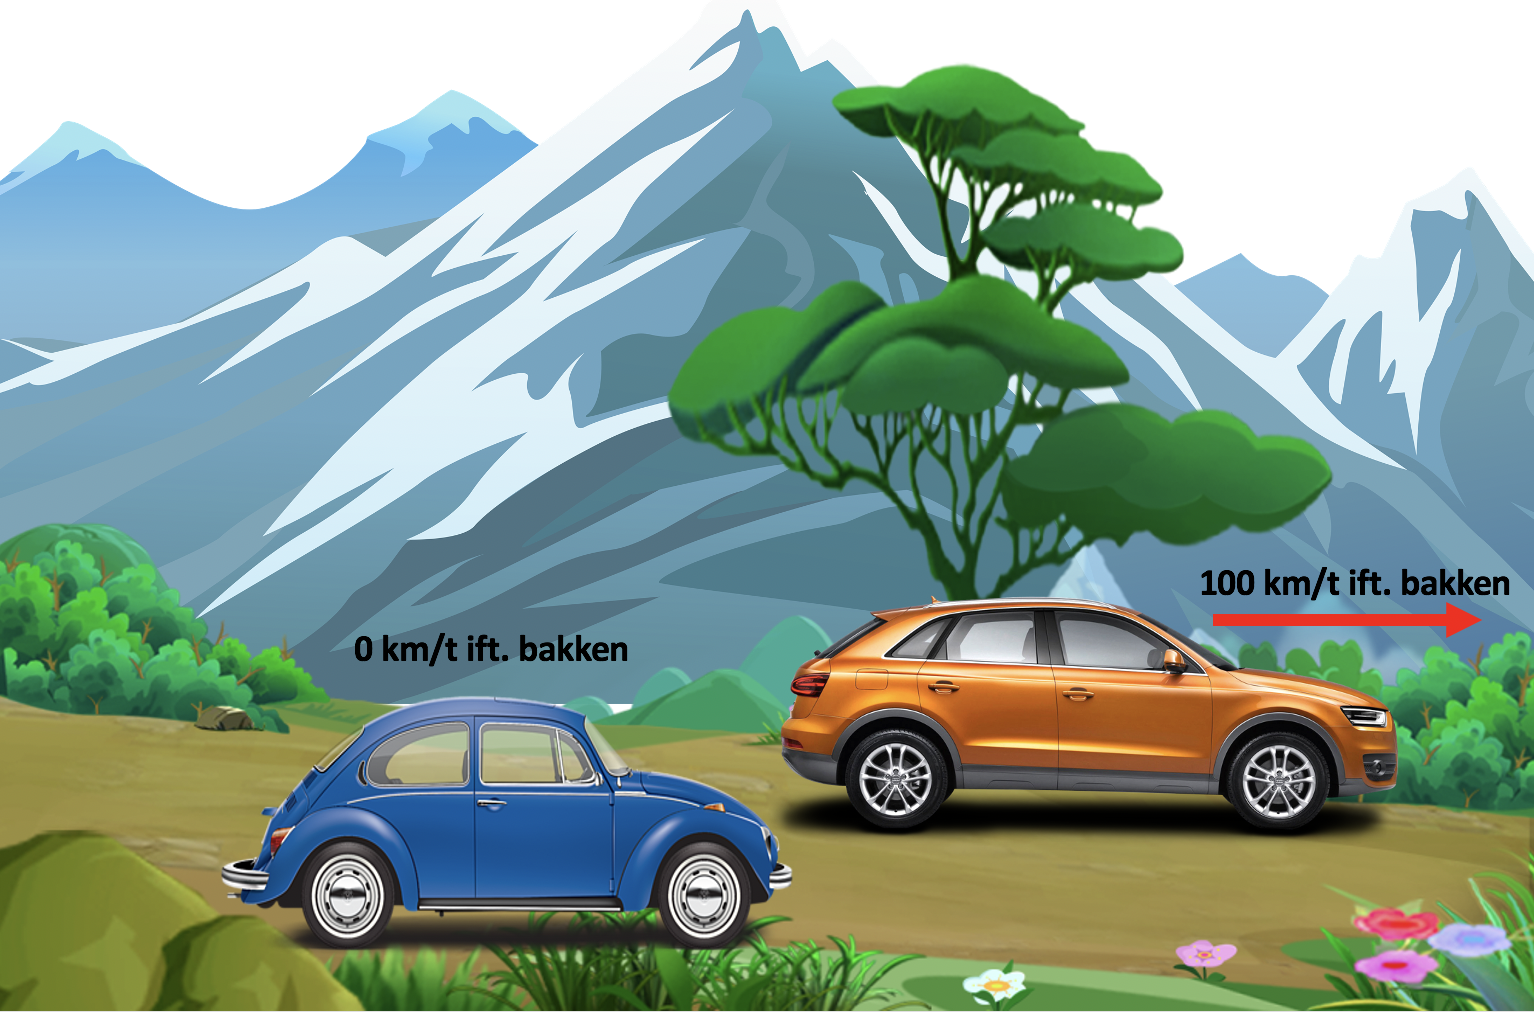
\includegraphics[scale=0.3]{media/klassrel1.png}}
{\small
Her ser vi en blå bil som står rolig i forhold til (ift) bakken ({\bf merk} hastigheter må alltid angies {\bf i forhold til} noe). Den oransje bilen beveger seg med 100 km/t i forhold til bakken og den blå bilen.\\
{\tiny Figurene i dette dokumentet er png-er fra hiclipart.com som har blitt satt sammen og mikset}
}
}{SIDE 1/23/61}

\choiceframe{kr2}{kr1}{0}{
\centerline{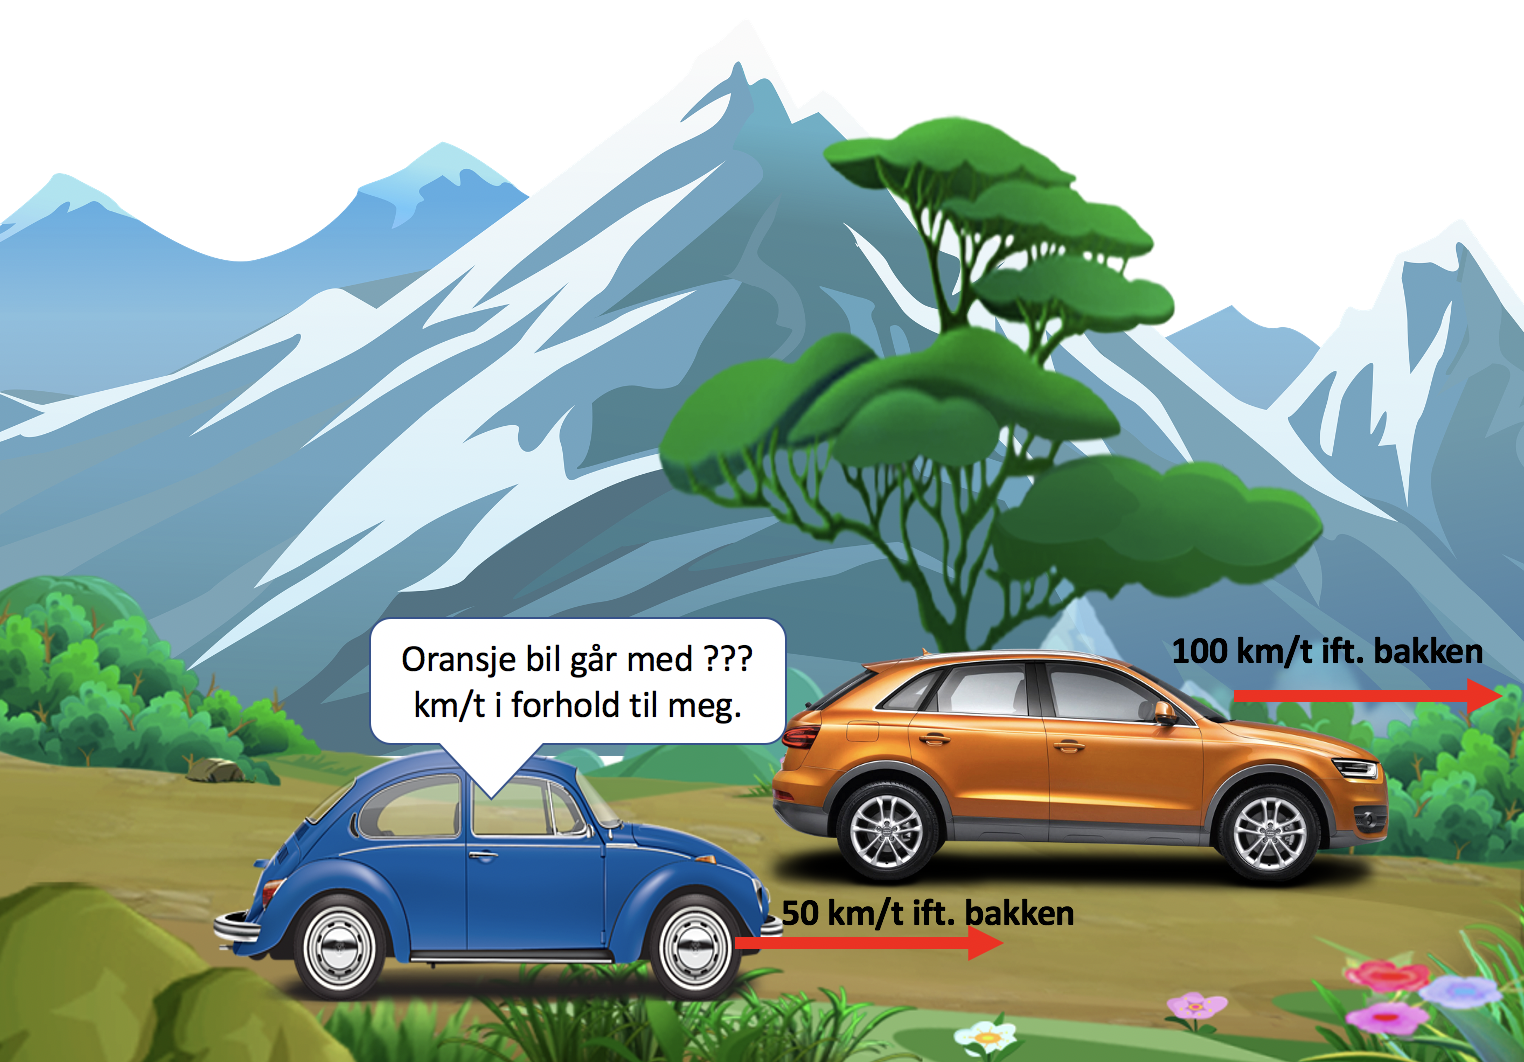
\includegraphics[scale=0.3]{media/klassrel2.png}}
{\small
Nå har den blå bilen starten motoren slik at den har en fart på 50 km/t i forhold til bakken. Den oransje bilen har enda 100 km/t i forhold til bakken. \textcolor{red}{Hvilken hastighet har den oransje bilen i den blå bilens referansesystem? {\bf Et referansesystem er et sett av observatører som alle er i ro i forhold til hverandre og derfor vil være enige om hastighetsmålinger av objekter}.}\\
\hyperlink{feil_kr2a}{\choicebutton{-100 km/t}}\hyperlink{feil_kr2a}{\choicebutton{-50 km/t}}\hyperlink{feil_kr2a}{\choicebutton{0 km/t}}\hyperlink{riktig_kr2b}{\choicebutton{50 km/t}}\hyperlink{feil_kr2a}{\choicebutton{100 km/t}}
}
}{SIDE 2/23/61}

\colchoiceframe{feil_kr2a}{kr2}{0}{black}{\Huge
\textcolor{yellow}{Det ble galt! Er du sikker på at du kikket skikkelig på figuren? Hvordan var klassisk relativitet? Hva må du gjøre for å finne den oransje bilens hastighet i forhold til den blå? Tenk en gang til og prøv igjen!}
}{SIDE 3/23/61}

\colfullframe{riktig_kr2b}{kr2}{kr3}{-1}{yellow}{\huge
\centerline{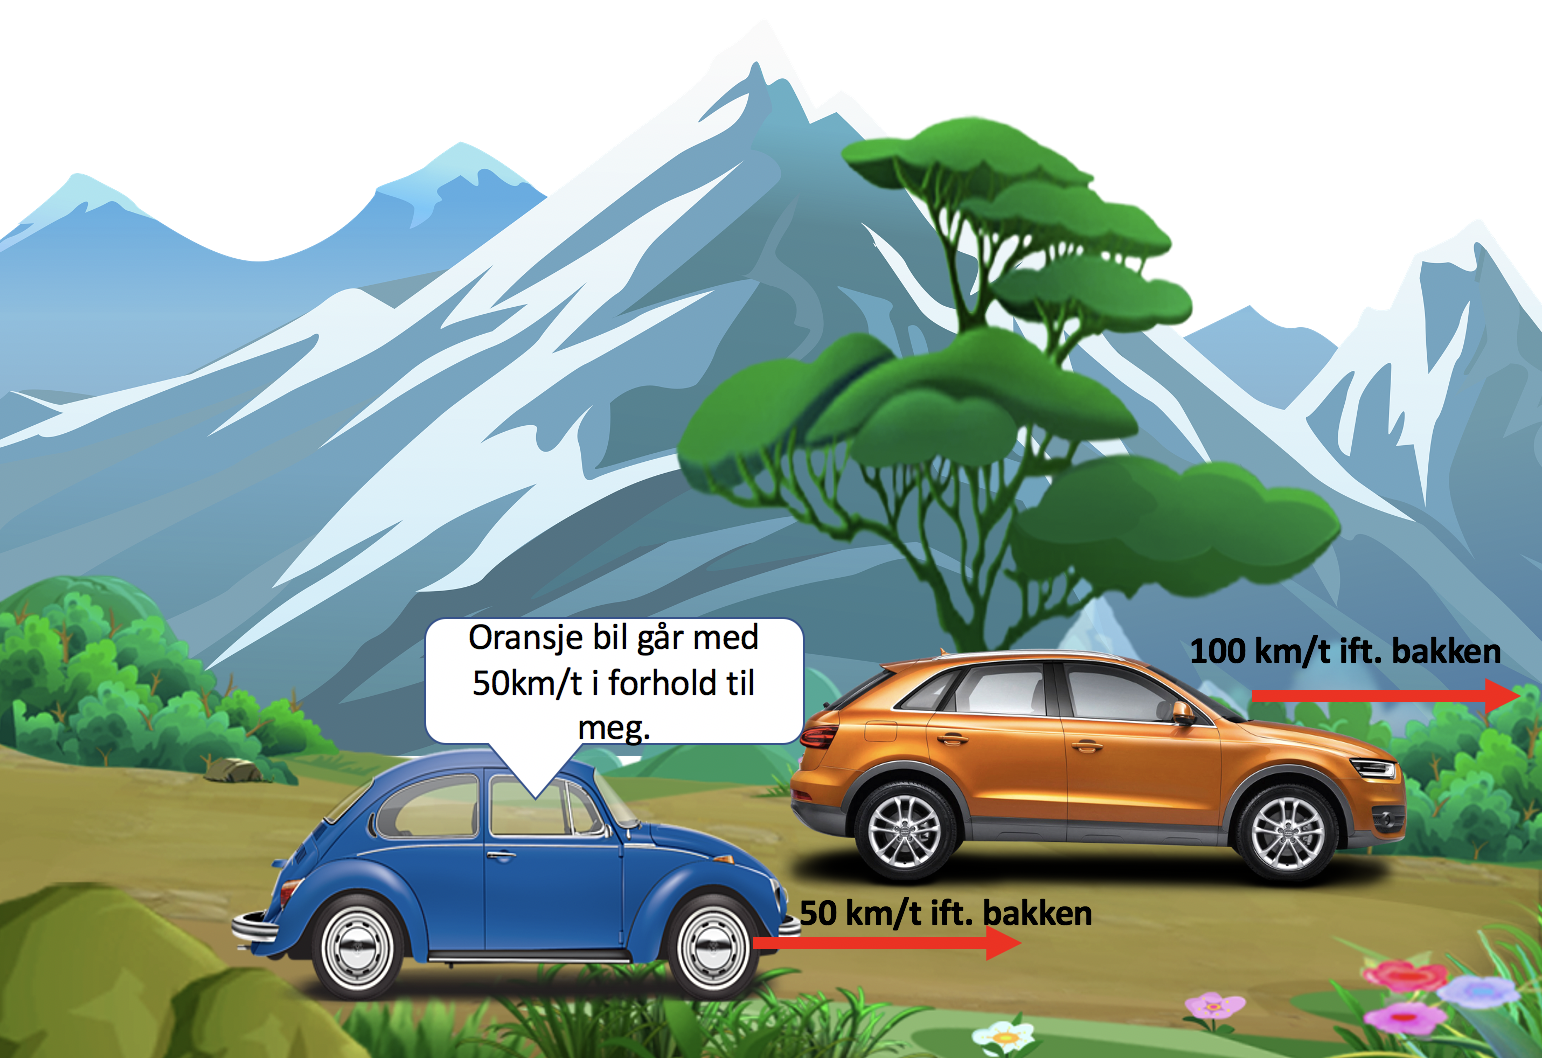
\includegraphics[scale=0.3]{media/klassrel3.png}}
Det er helt riktig! Brukte du intuisjon eller fant du en formel/sammenheng mellom de to hastighetene?
}{SIDE 4/23/61}


\choiceframe{kr3}{riktig_kr2b}{0}{
\centerline{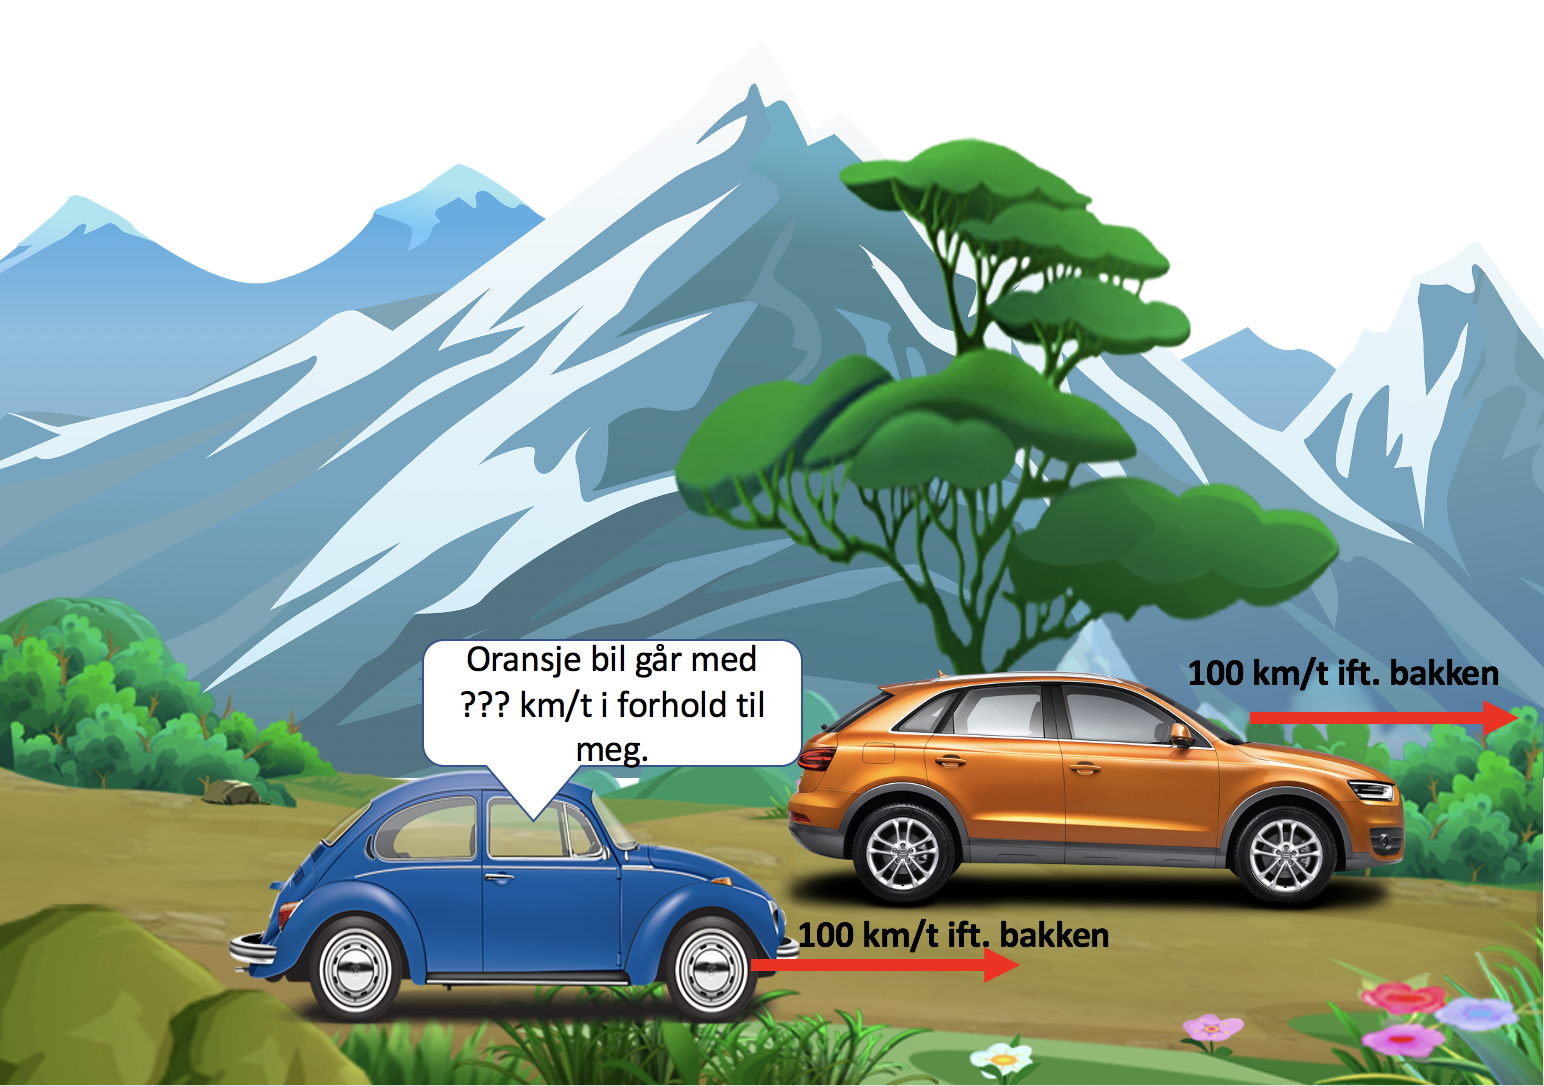
\includegraphics[scale=0.3]{media/klassrel4.png}}
{\small
Hva nå hvis den blå bilen øker til 100 km/t? Den oransje bilen har enda 100 km/t i forhold til bakken. Hvilken hastighet har den oransje bilen i den blå bilens referansesystem? {\bf Et referansesystem er et sett av observatører som alle er i ro i forhold til hverandre og derfor vil være enige om hastighetsmålinger av objekter}.\\
\hyperlink{feil_kr3a}{\choicebutton{-100 km/t}}\hyperlink{feil_kr3a}{\choicebutton{-50 km/t}}\hyperlink{riktig_kr3b}{\choicebutton{0 km/t}}\hyperlink{feil_kr3a}{\choicebutton{50 km/t}}\hyperlink{feil_kr3a}{\choicebutton{100 km/t}}
}
}{SIDE 5/23/61}


\colchoiceframe{feil_kr3a}{kr3}{0}{black}{\Huge
\textcolor{yellow}{Det ble galt! Er du sikker på at du kikket skikkelig på figuren? Går ikke begge bilene her med samme fart i forhold til bakken? Tenk en gang til og prøv igjen!}
}{SIDE 6/23/61}

\colfullframe{riktig_kr3b}{kr3}{kr4}{-1}{yellow}{\Large
\centerline{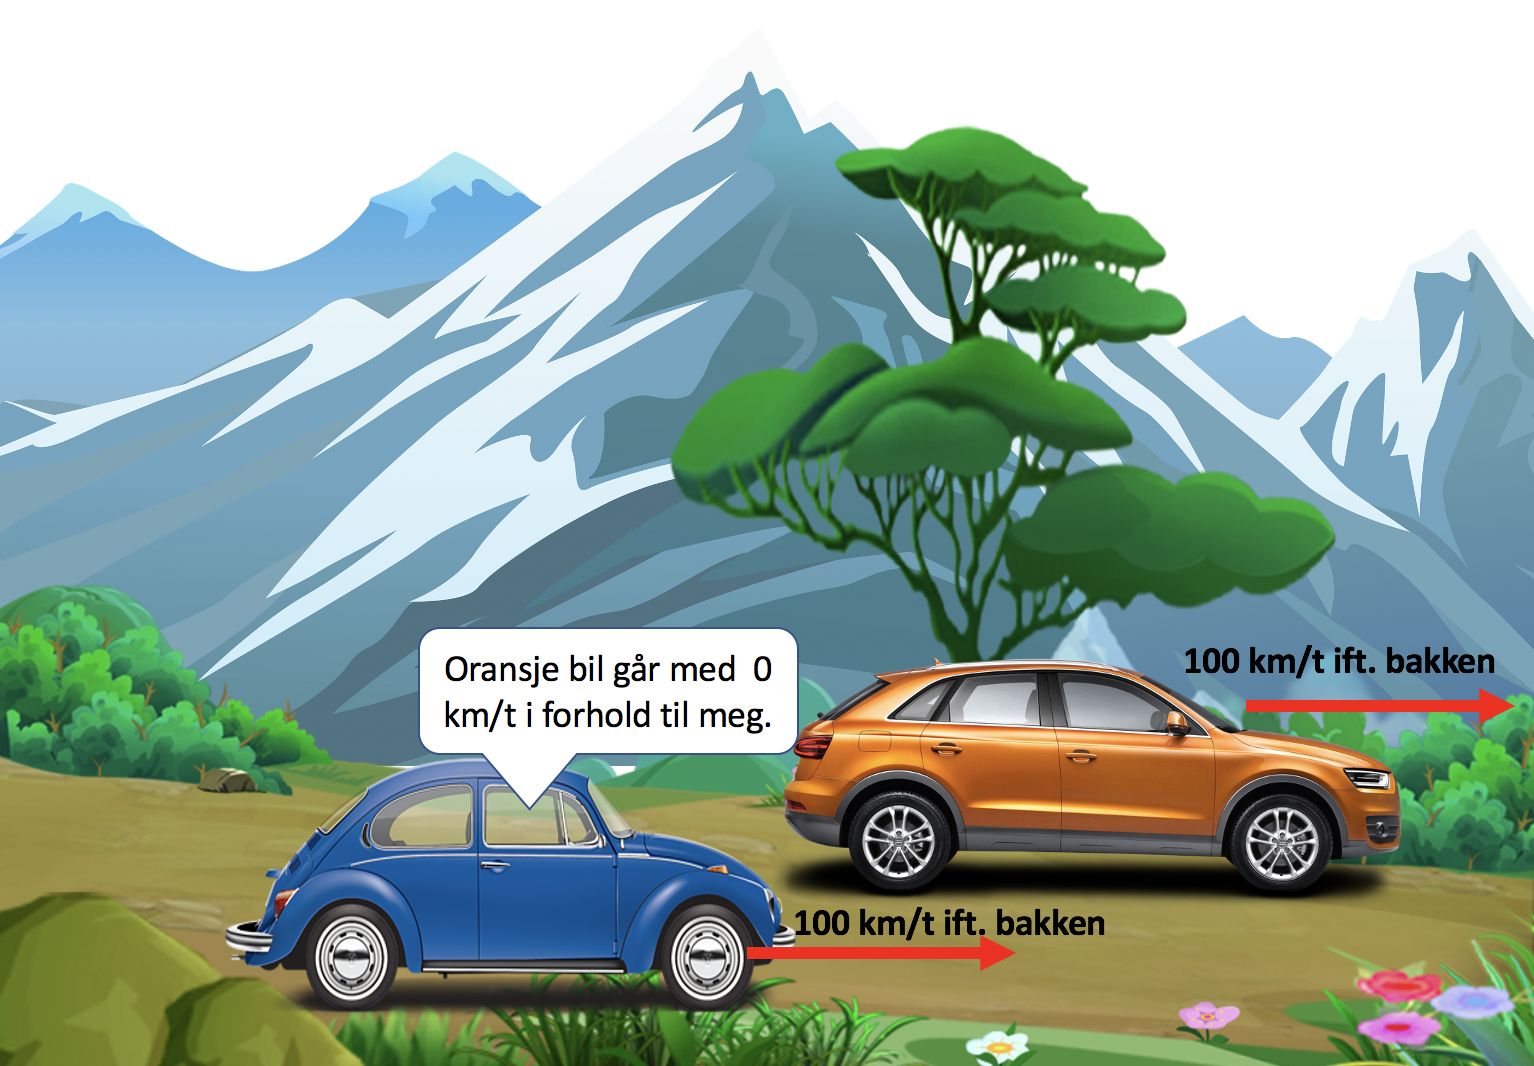
\includegraphics[scale=0.3]{media/klassrel5.png}}
Det er helt riktig! Brukte du intuisjon eller fant du en formel/sammenheng mellom de to hastighetene? Var det samme sammenheng som i forrige spørsmål?
}{SIDE 7/23/61}

\choiceframe{kr4}{riktig_kr3b}{0}{
\centerline{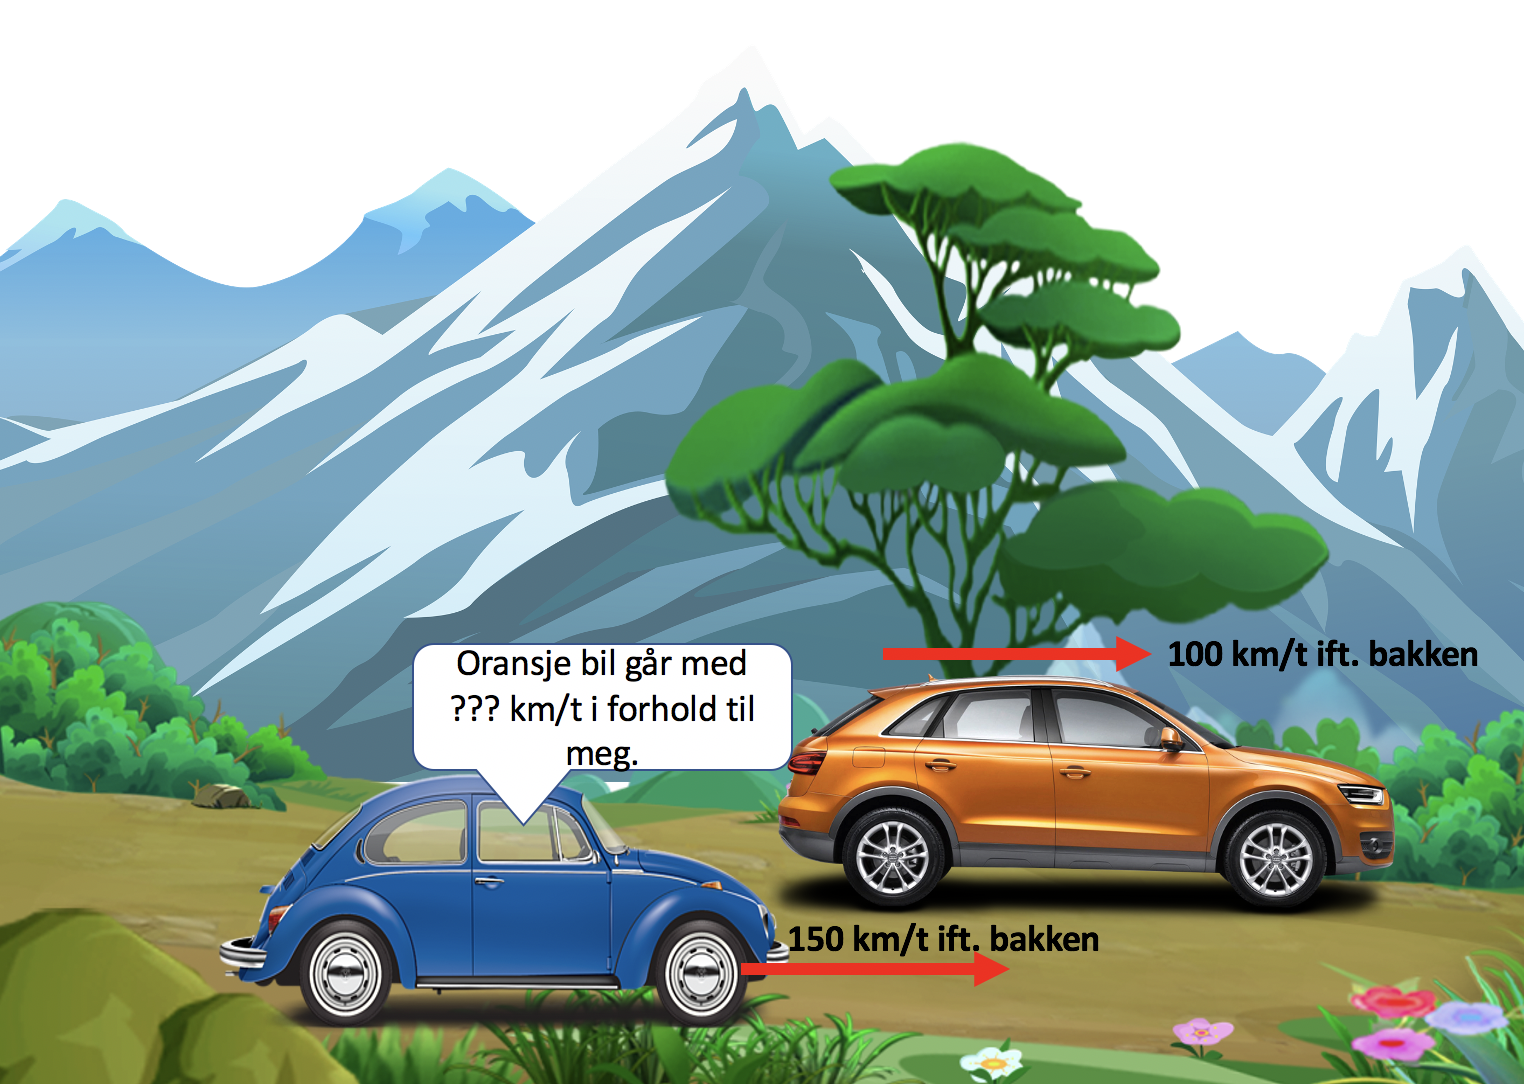
\includegraphics[scale=0.3]{media/klassrel6.png}}
{\small
Hva nå hvis den blå bilen øker til 150 km/t? Den oransje bilen har enda 100 km/t i forhold til bakken. Hvilken hastighet har den oransje bilen i den blå bilens referansesystem? \textcolor{red}{\bf Et referansesystem er et sett av observatører som alle er i ro i forhold til hverandre og derfor vil være enige om hastighetsmålinger av objekter}.\\
\hyperlink{feil_kr4a}{\choicebutton{-150 km/t}}\hyperlink{riktig_kr4b}{\choicebutton{-50 km/t}}\hyperlink{feil_kr4a}{\choicebutton{0 km/t}}\hyperlink{feil_kr4a}{\choicebutton{50 km/t}}\hyperlink{feil_kr4a}{\choicebutton{150 km/t}}
}
}{SIDE 8/23/61}

\colchoiceframe{feil_kr4a}{kr4}{0}{black}{\huge
\textcolor{yellow}{Er du heeeelt sikker!Har  du kikket skikkelig på figuren? Går ikke blå fortere enn oransje? Hvis du sitter i en bil og kjører fortere enn bilen ved siden av, hvis du betrakter deg selv om i ro, hva er farten til den andre bilen? Tenk en gang til og prøv igjen!}
}{SIDE 9/23/61}

\colfullframe{riktig_kr4b}{kr4}{kr5}{-1}{yellow}{\Large
\centerline{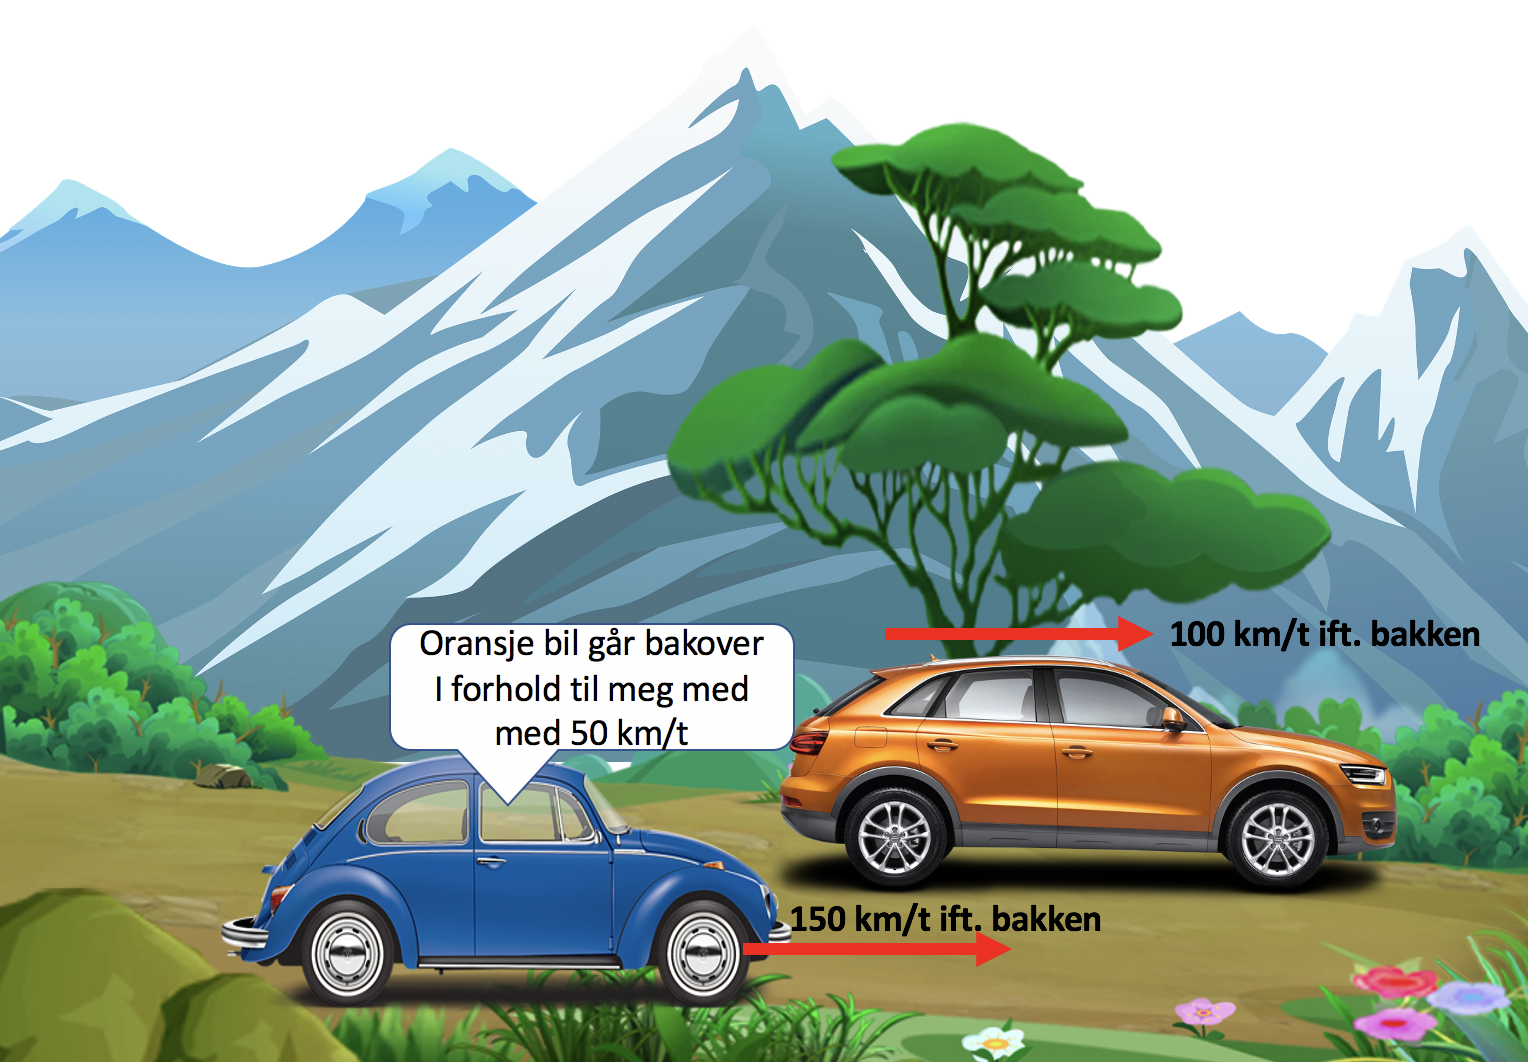
\includegraphics[scale=0.3]{media/klassrel7.png}}
Det er helt riktig! Brukte du intuisjon eller fant du en formel/sammenheng mellom de to hastighetene? Var det samme sammenheng som i forrige spørsmål?
}{SIDE 10/23/61}


\fullframe{kr5}{riktig_kr4b}{kr6}{0}{
\centerline{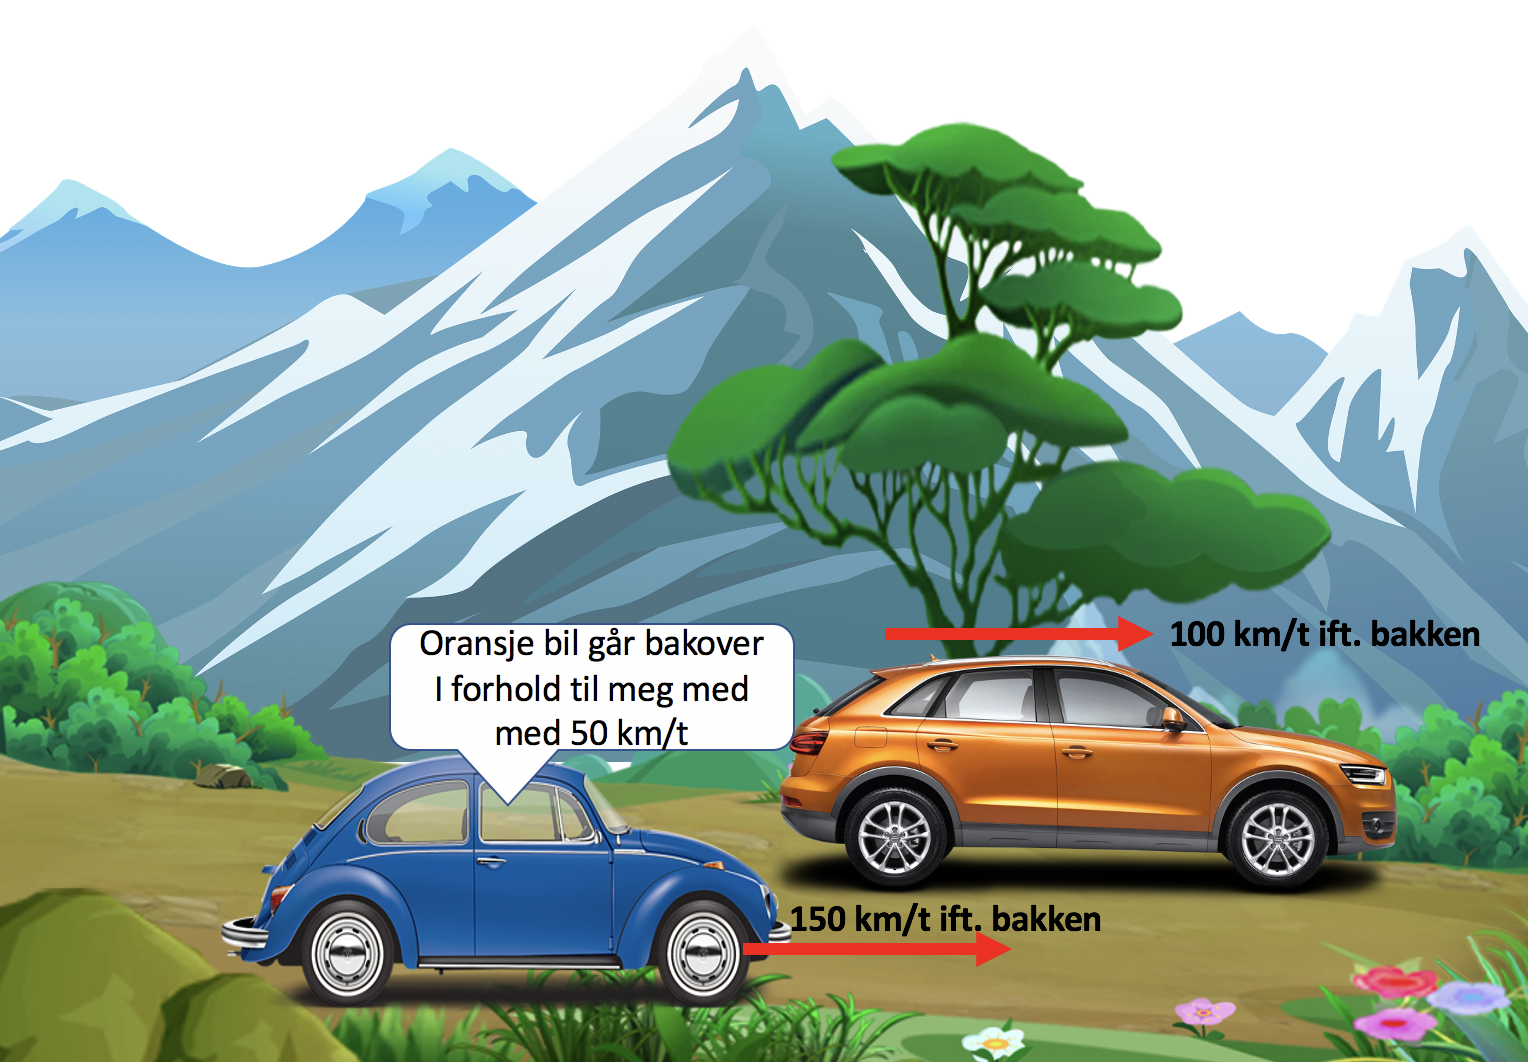
\includegraphics[scale=0.3]{media/klassrel7.png}}
{\small
Kom du frem til formelen for klassisk relativitet? Ble de noe sånt som:
\[
v'_\mathrm{oransje}=v_\mathrm{oransje}-v_\mathrm{rel}
\]
der merkede hastigheter er hastigheter målt i blått bil sitt referansesystem, umerkede hastigheter er målt i bakken sitt referansesystem og $v_\mathrm{rel}$ er den relative hastigheten mellom de to referansesystemene? Positiv hastighet måles til høyre.Stemmer det med det du fant?
}
}{SIDE 11/23/61}

\fullframe{kr6}{kr5}{kr7}{0}{
\centerline{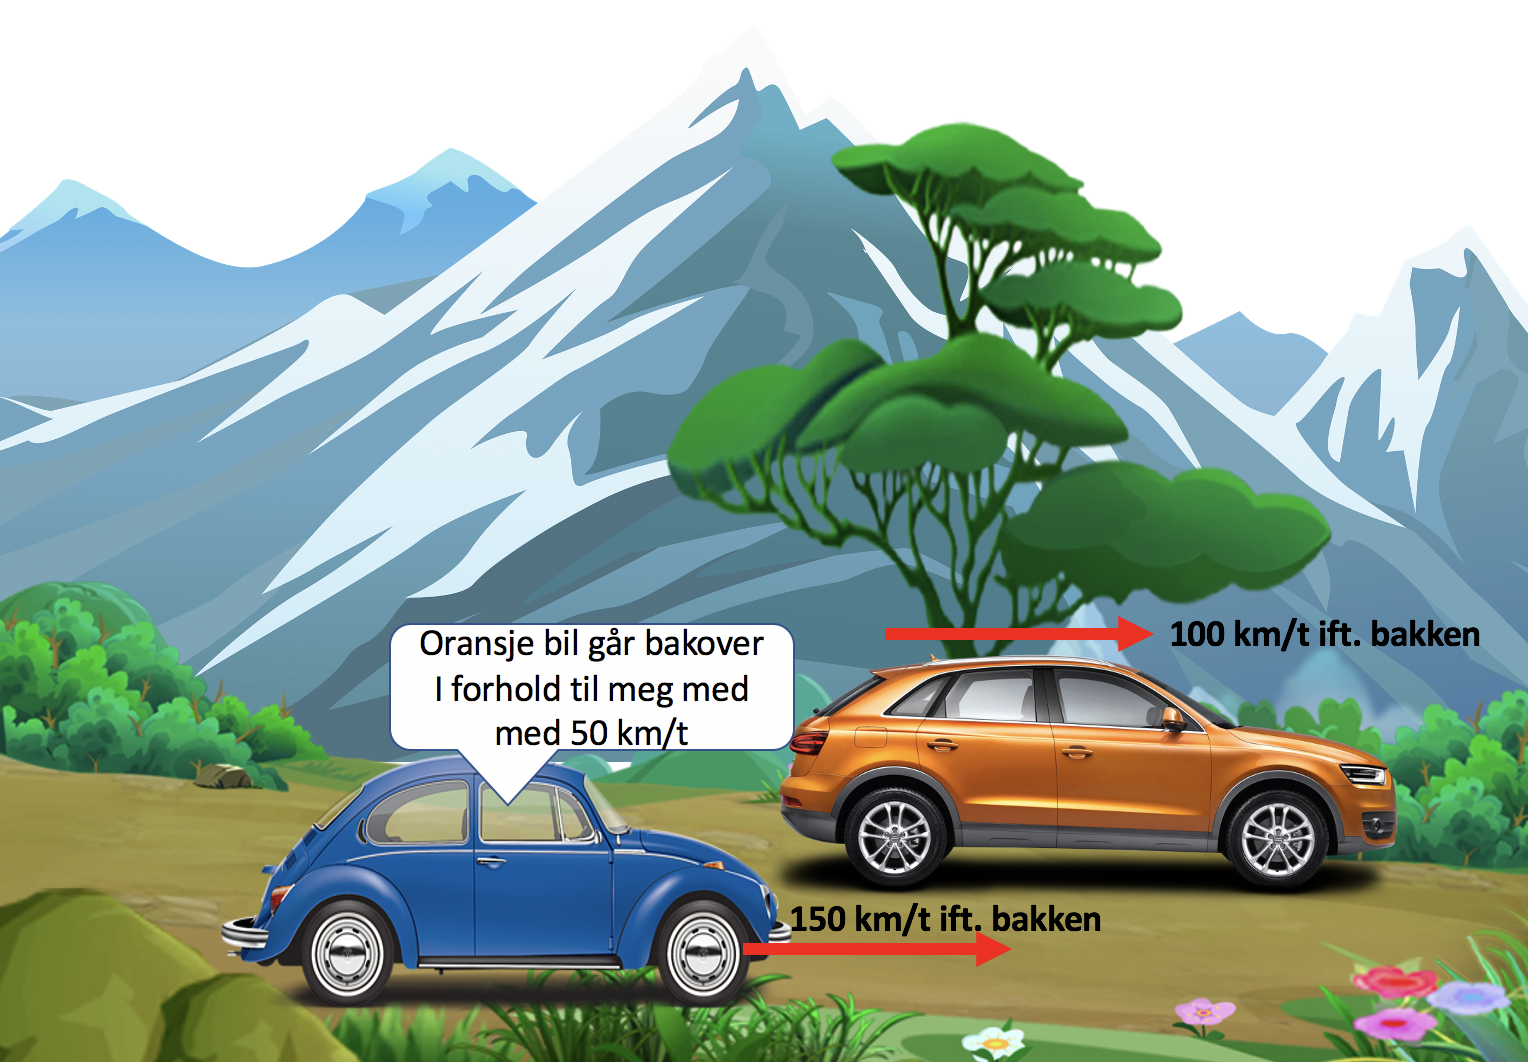
\includegraphics[scale=0.3]{media/klassrel7.png}}
{\small
La oss prøve:
\[
v'_\mathrm{oransje}=v_\mathrm{oransje}-v_\mathrm{rel}
\]
Farta til blå bils referansesysteme i forhold til bakkesystem er 150 km/t til høyre, altså er $v_\mathrm{rel}=150$ km/t. Farta til oransje bil i bakkesystem er $v_\mathrm{oransje}=100$ km/t. Setter vi inn, så får vi at oransje bil sin fart i blå bils referansesystem er  $v'_\mathrm{oransje}=-50$ km/t.
}
}{SIDE 12/23/61}


\fullframe{kr7}{kr6}{kr8}{0}{
{\bf La oss prøve den på lys:}
\centerline{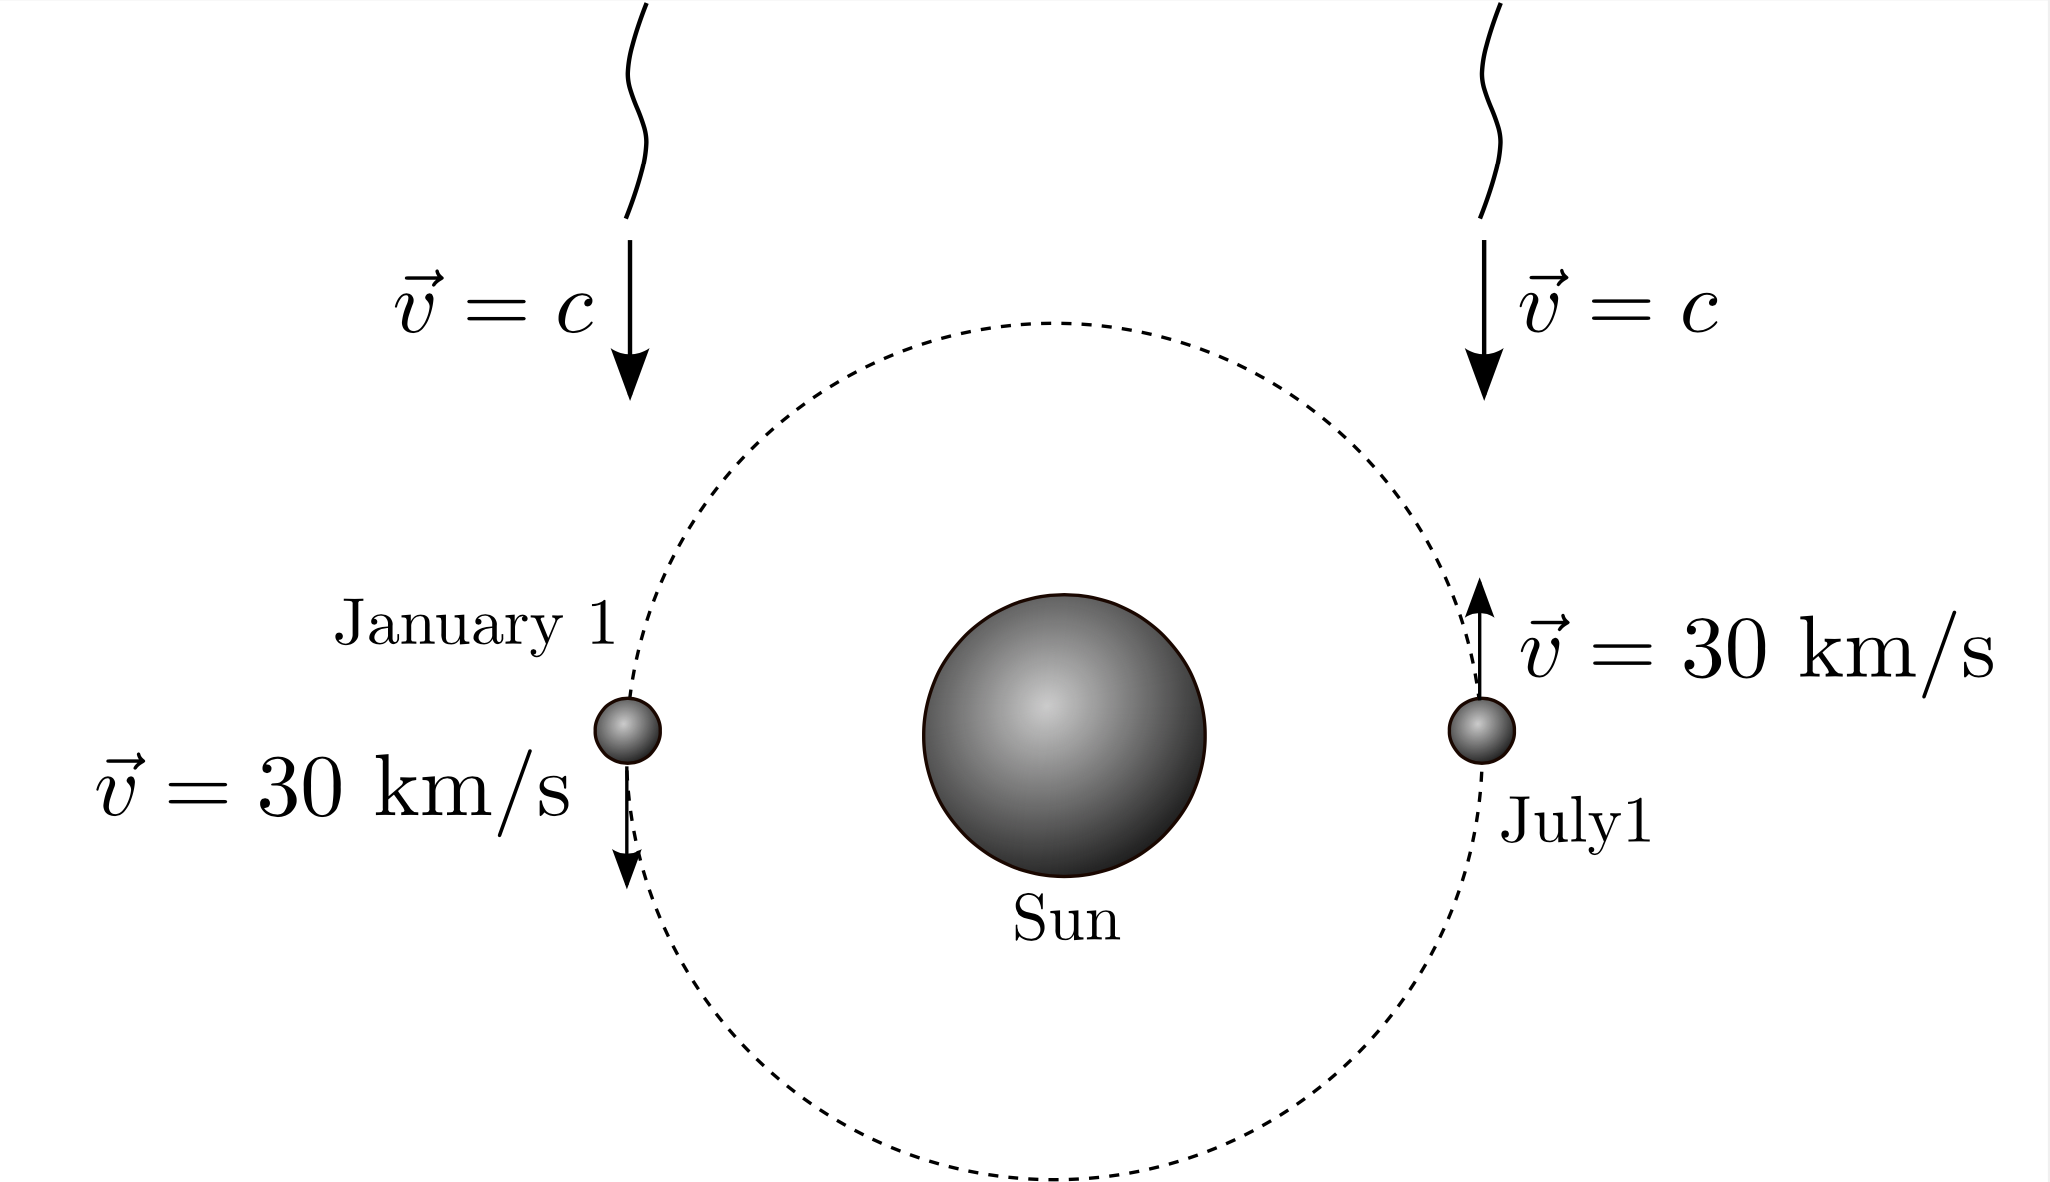
\includegraphics[scale=0.55]{media/fig_7-3.png}}
Dette er det klassiske {\bf Michelson-Morley-eksperimentet.} Der ble farta til lys i forhold til jorda sitt referansesystem målt. Lys blir sendt ut fra en fjern stjerne mot jorda. Vi antar at stjerna er i samme referansesystem som sola. Det ble sendt ut med lyshastighet $c=300 000$ km/s. Anta at farta til dette lyset så blir målt på jorda i forhold til jordas referansesystem, først den 1.januar når jorda er på vei {\bf bort fra} lysstrålen, og så 1.juli når jorda er på vei {\bf mot} lysstrålen.

}{SIDE 13/23/61}



\choiceframe{kr8}{kr7}{0}{
\centerline{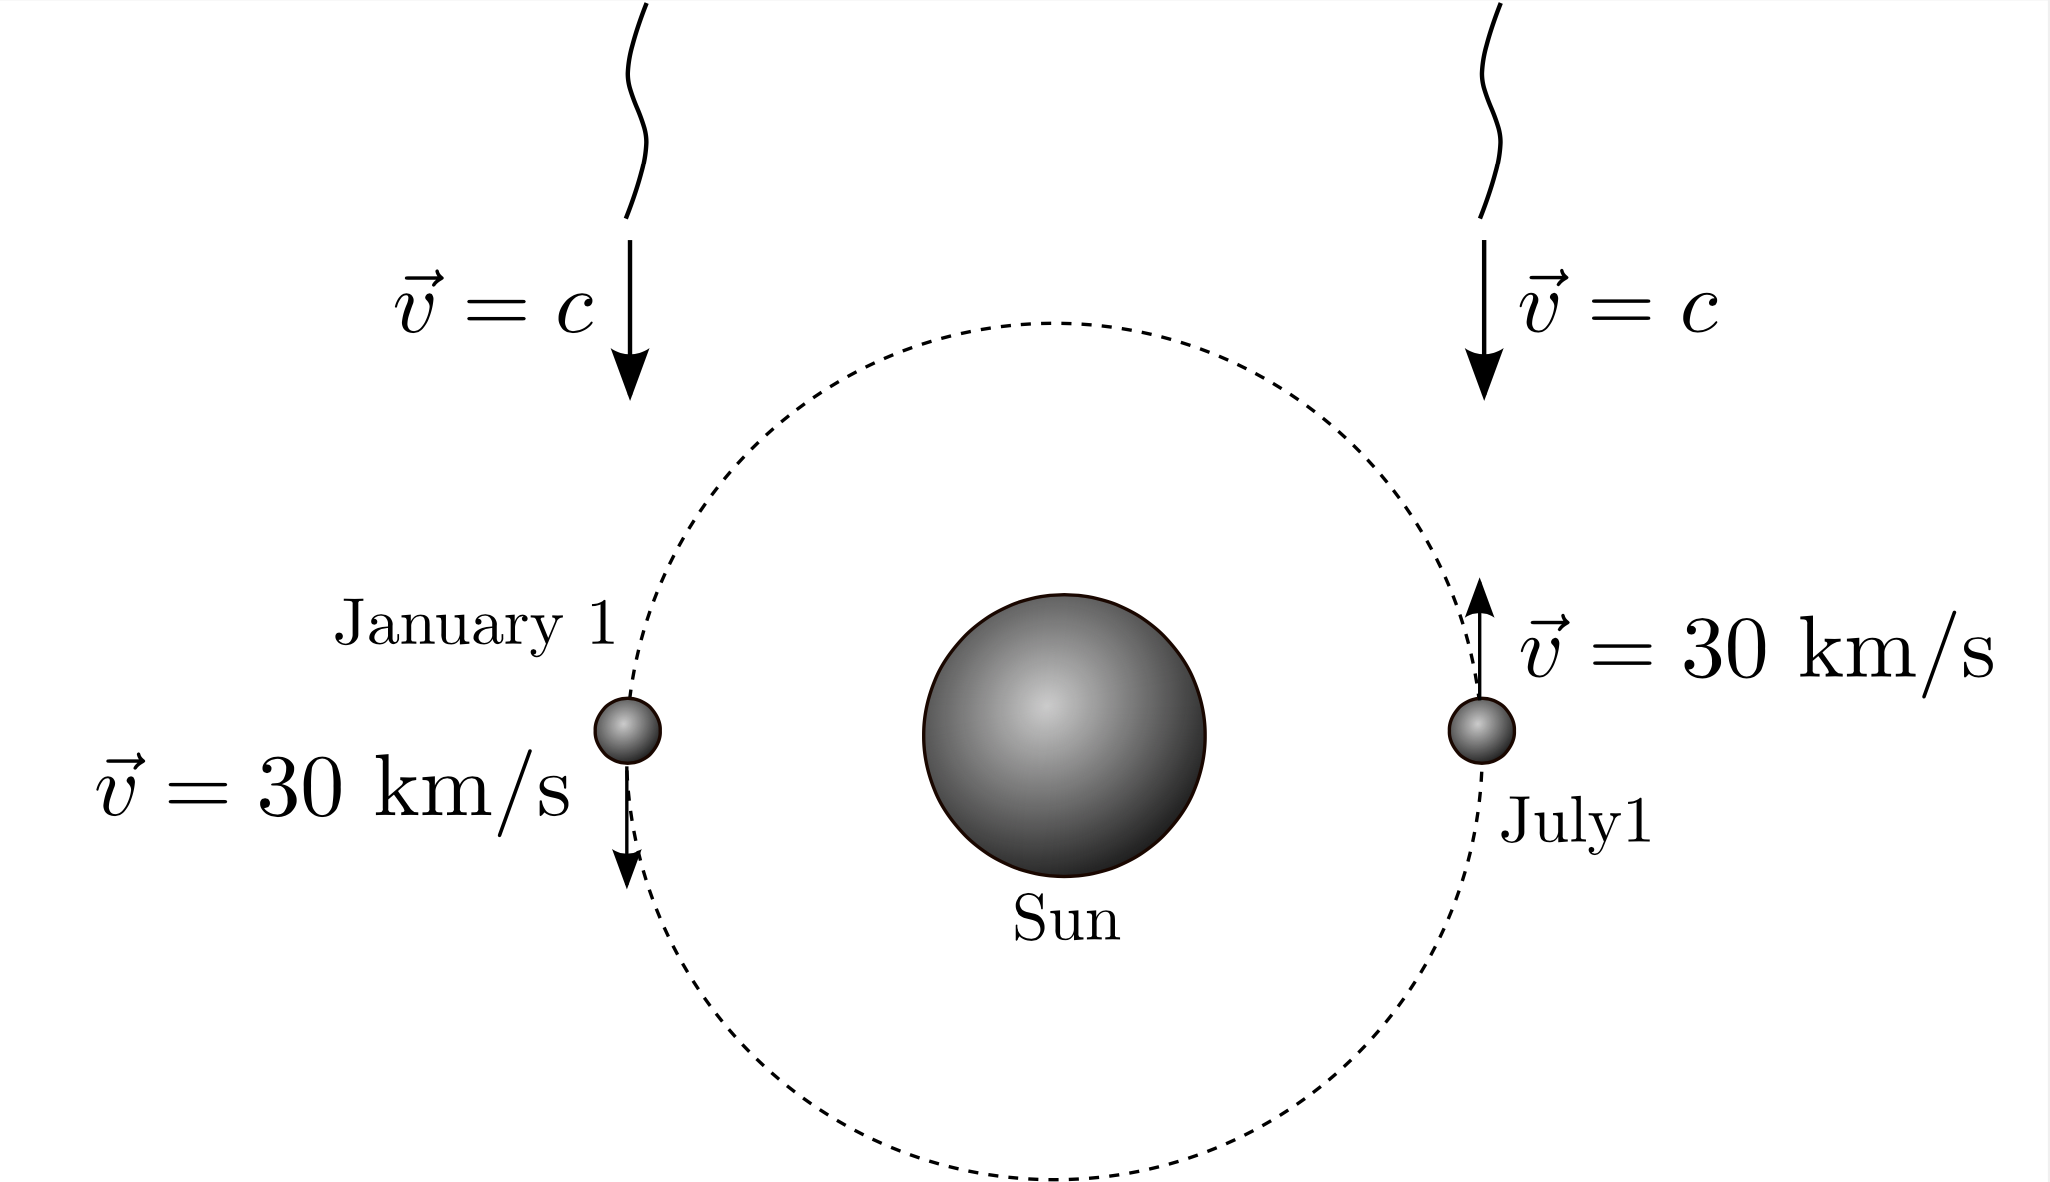
\includegraphics[scale=0.55]{media/fig_7-3.png}}

Hvis vi bruker klassisk relativitet og glemmer Einstein litt, hvilken fart måler man for lyset i jordas referansesystem den 1.januar? Jordas banehastighet er ca. 30 km/s i forhold til solas (og stjernas) referansesystem.
\hyperlink{riktig_kr8b}{\choicebutton{c - 30km/s}}\hyperlink{feil_kr8a}{\choicebutton{\ \ c\ \ }}\hyperlink{feil_kr8a}{\choicebutton{c + 30km/s}}
}{SIDE 14/23/61}

\colchoiceframe{feil_kr8a}{kr8}{0}{black}{\large
\textcolor{yellow}{Kan det blir riktig? Vi beveger oss i samme retning som lyset! Hvordan var det når den blå bilen beveget seg i samme retning som den oransje men med lavere fart?}
}{SIDE 15/23/61}

\colfullframe{riktig_kr8b}{kr8}{kr9}{-1}{yellow}{
\centerline{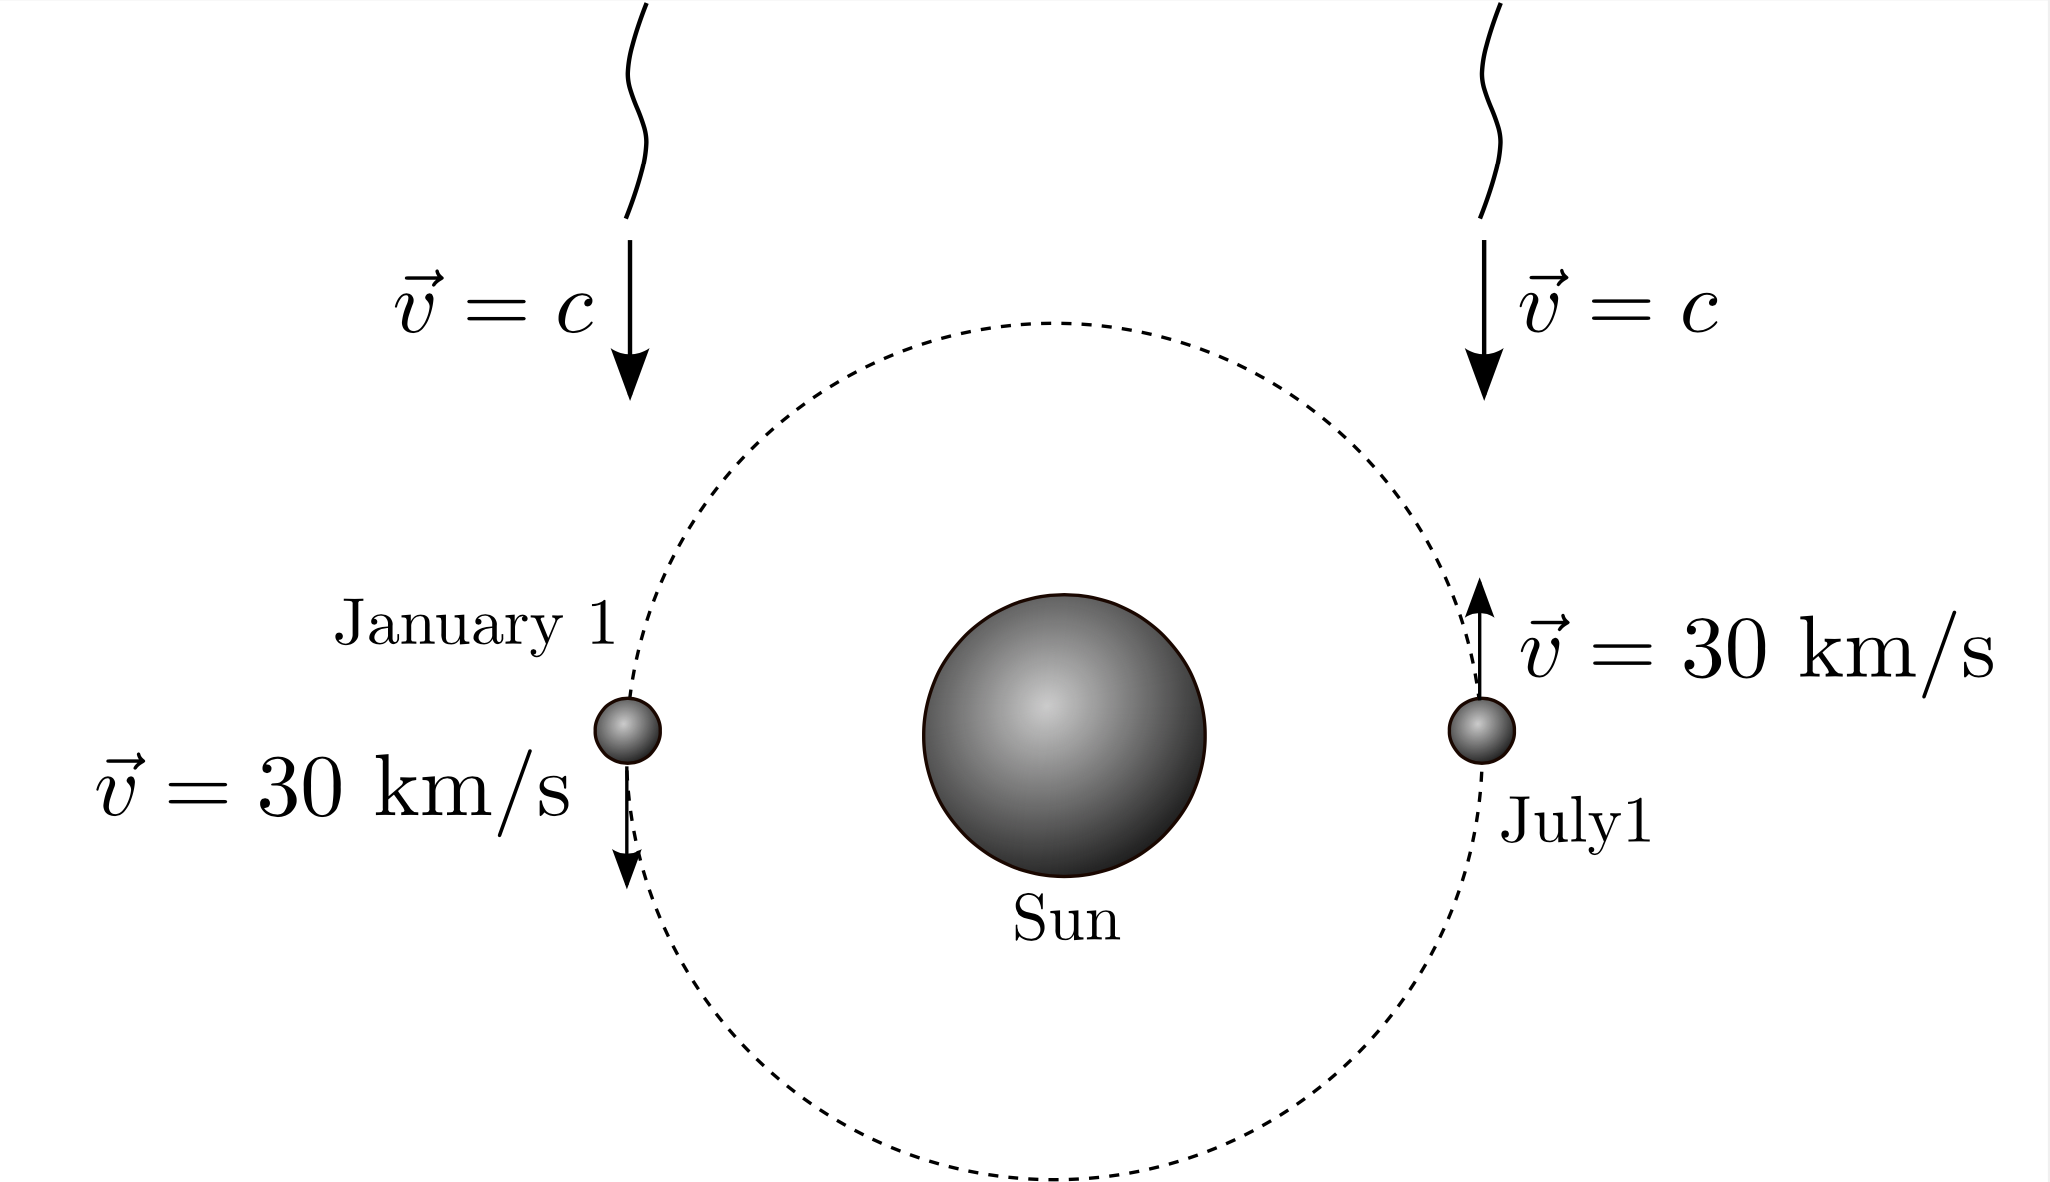
\includegraphics[scale=0.55]{media/fig_7-3.png}}
Det er helt riktig!
\[
v'_\mathrm{lys}=v_\mathrm{lys}-v_\mathrm{rel}
\]
Hvis vi nå bruker positiv hastighet nedover: referansesystemet til jorda beveger seg i positiv retning med 30 km/s i forhold til sola/stjernas referansesystem, da er relativ hastighet mellom systemer $v_\mathrm{rel}=30$km/s. Jorda sitt referansesystem er merket, sola sitt er umerket. I sola sitt system er lysets hastighet $c$. Da får vi at $v'_\mathrm{lys}=c-30$km/s i jorda sitt system.
}{SIDE 16/23/61}

\fullframe{kr9}{riktig_kr8b}{kr10}{0}{
\centerline{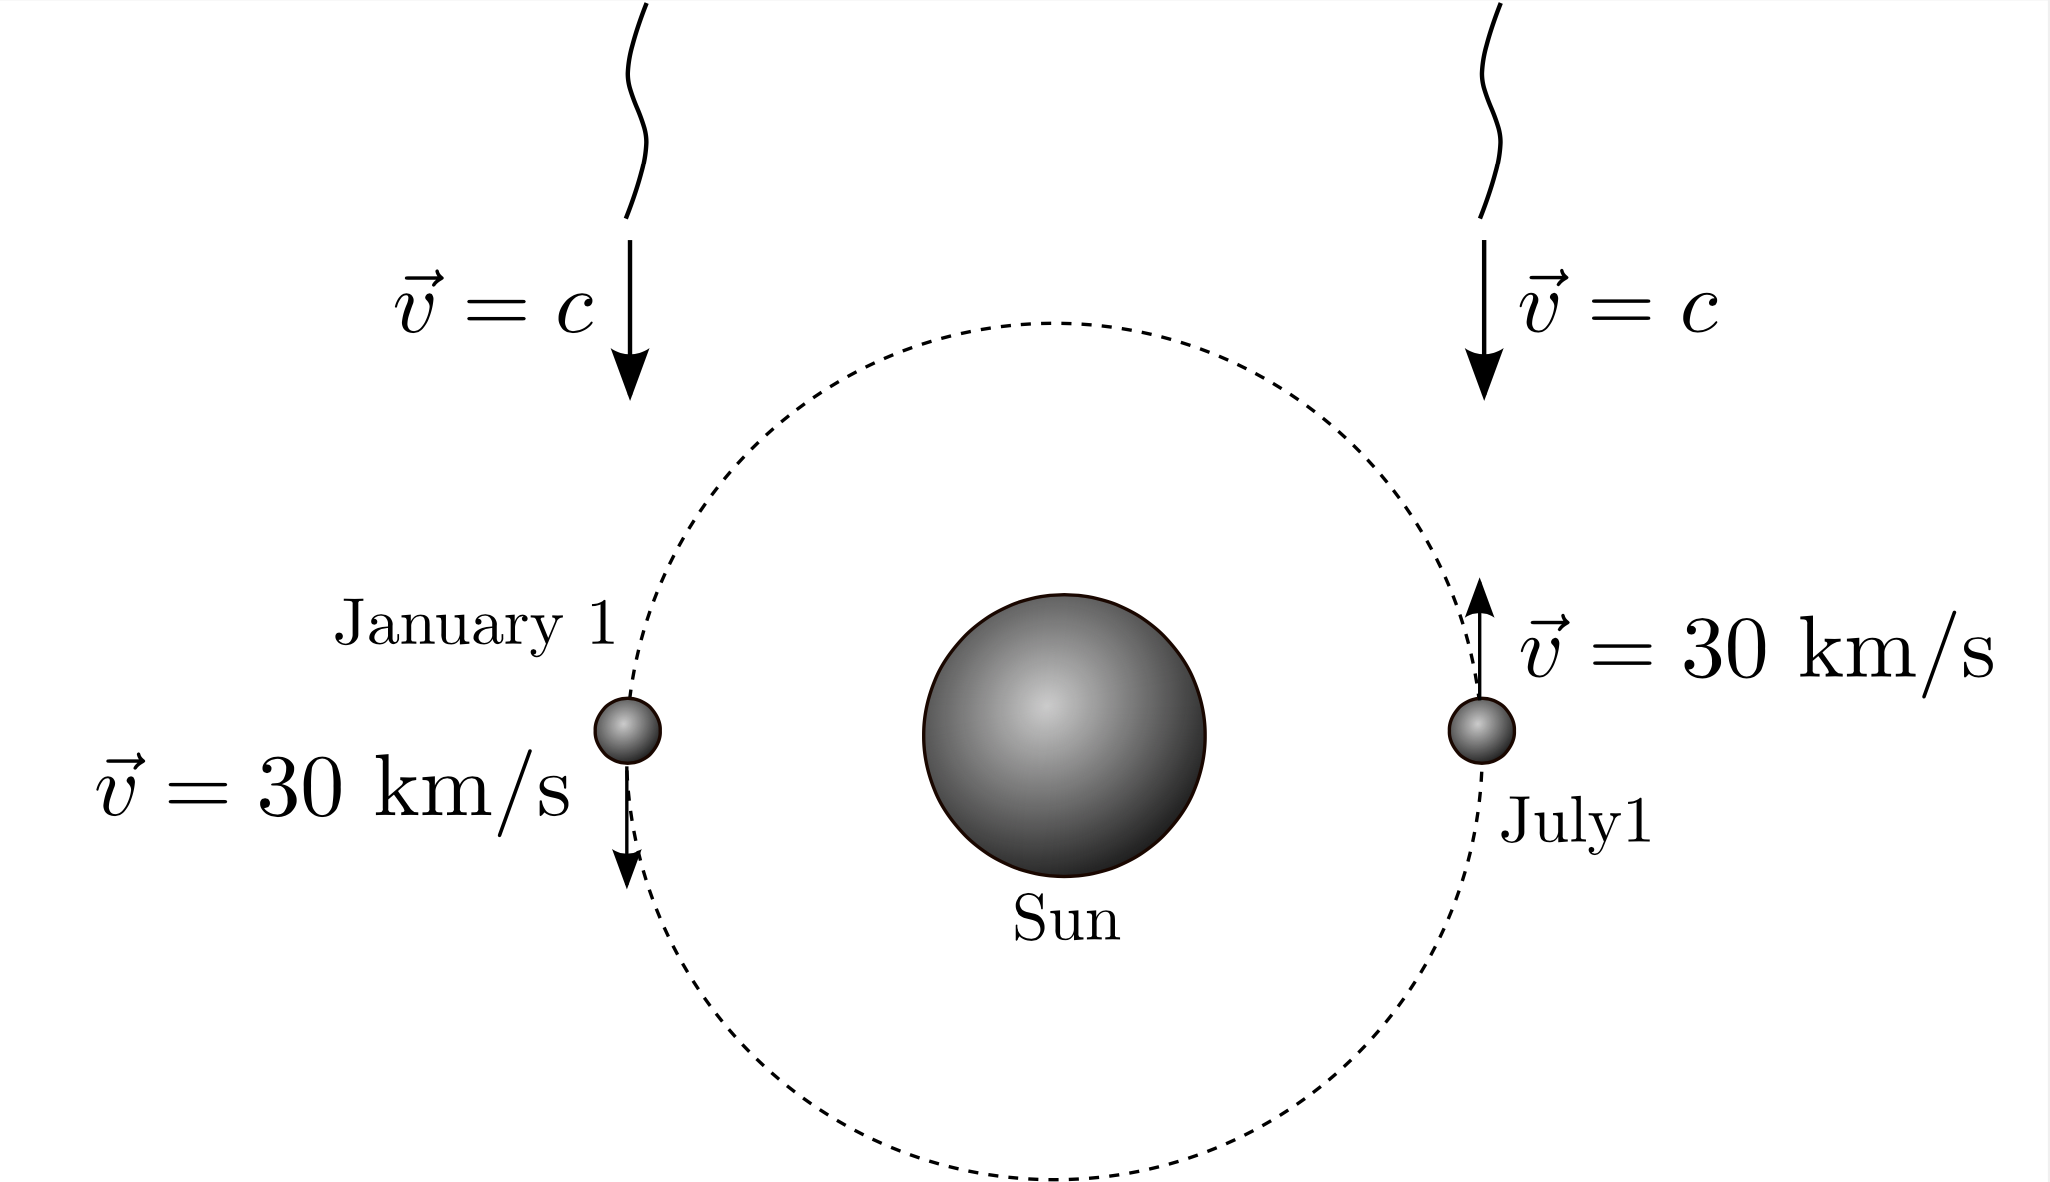
\includegraphics[scale=0.55]{media/fig_7-3.png}}
\[
v'_\mathrm{lys}=v_\mathrm{lys}-v_\mathrm{rel}
\]
Vi kan bruke akkurat samme resonnement for 1.juli, men da er hastigheten til jorda sitt referansesystem negativ, altså $v_\mathrm{rel}=-30$km/s som gir $v'_\mathrm{lys}=c+30$km/s. Mens vi den 1.januar skulle målt  $v'_\mathrm{lys}=c-30$km/s. Dvs. at hvis klassisk relativitet er riktig, skulle vi målt forskjellig hastighet for lyset på de to forskjellige datoene. Det Micheleson og Morley fant var at lyshastigheten var den samme.
}{SIDE 17/23/61}



\fullframe{kr10}{kr9}{kr11}{0}{\small
\centerline{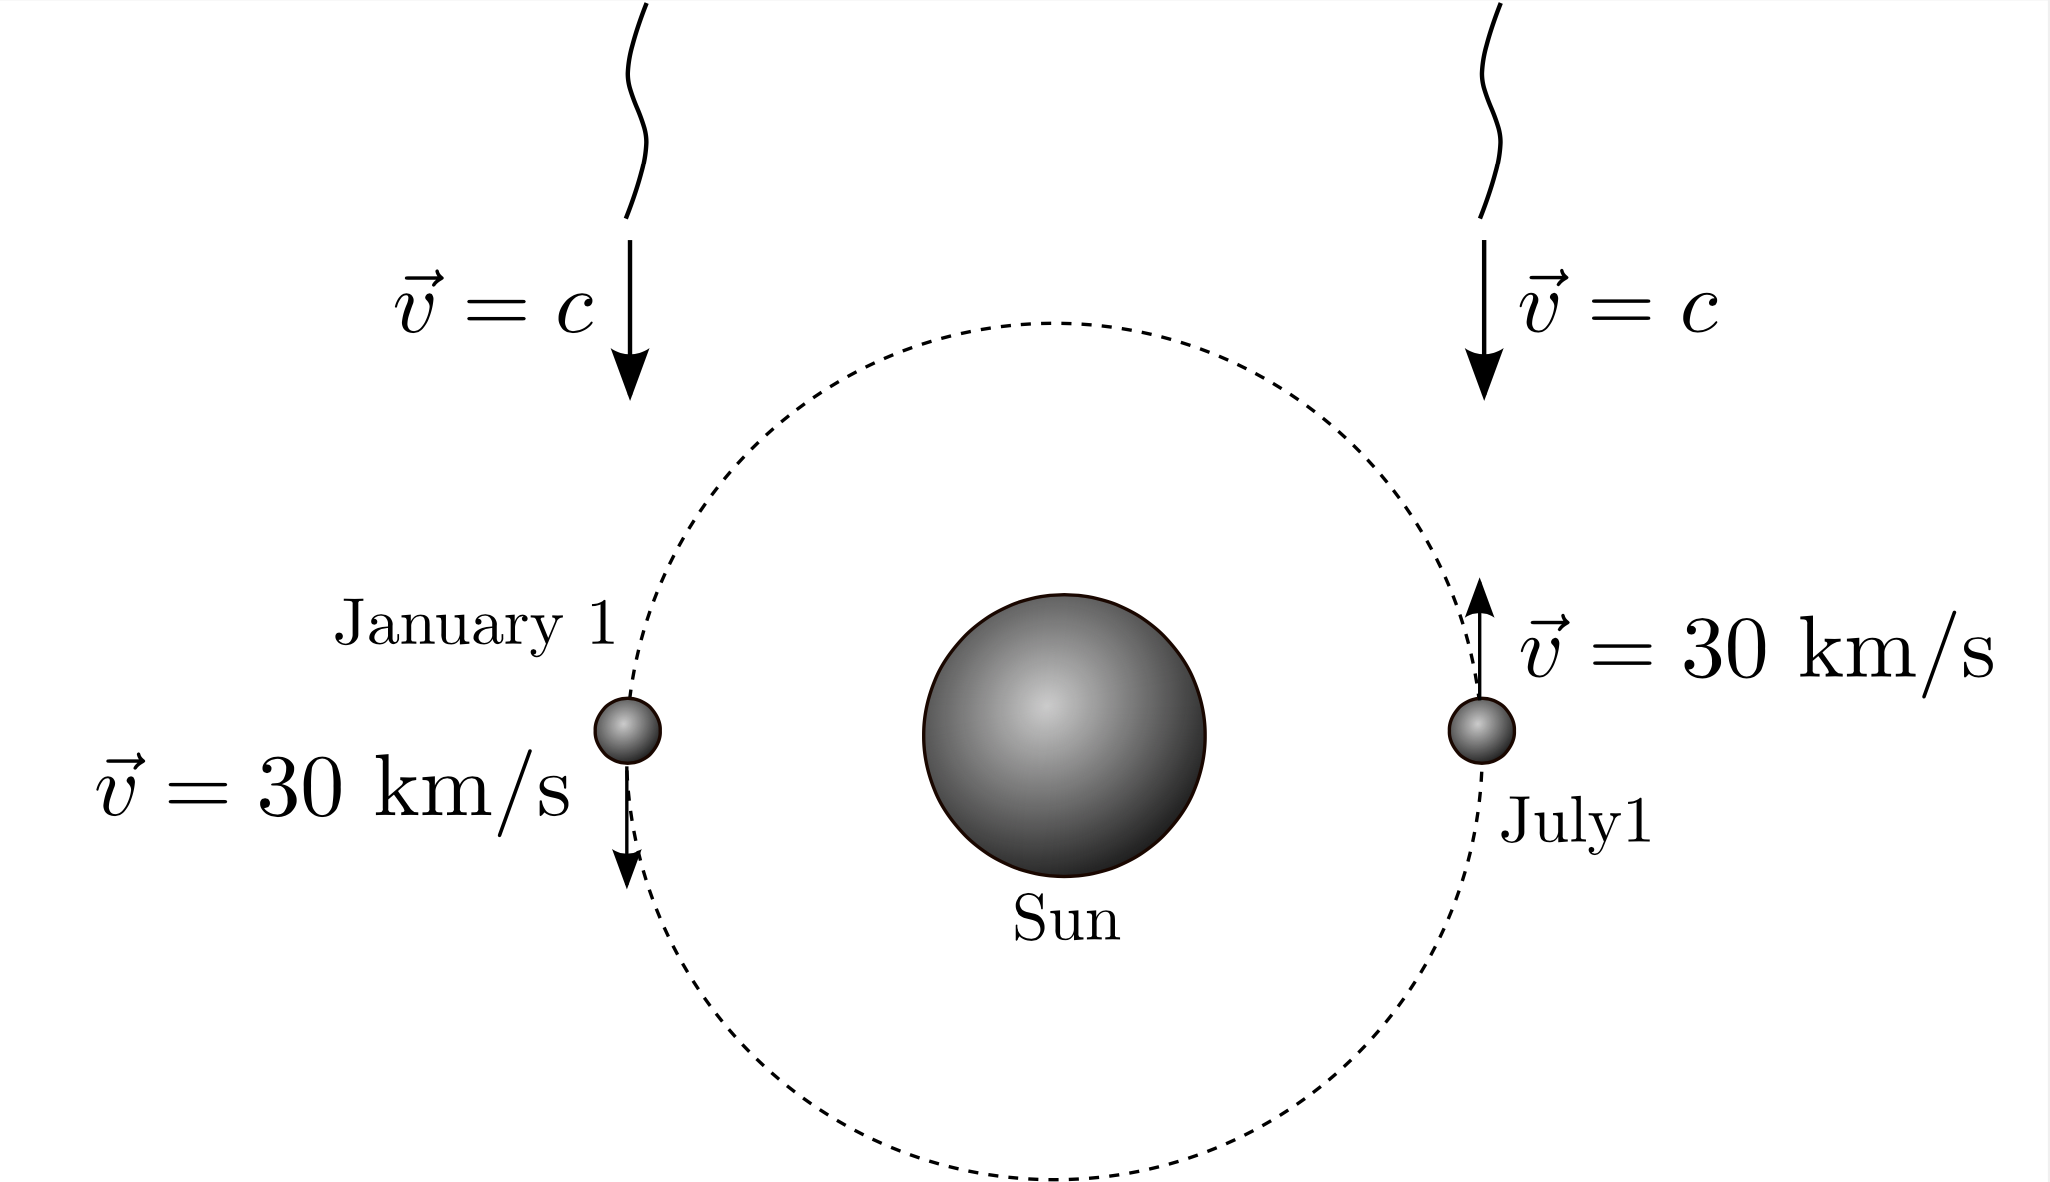
\includegraphics[scale=0.55]{media/fig_7-3.png}}
{\bf Akkurat dette var Einsteins utgangspunkt da han oppdaget relativitetsteorien. Han spurte seg hva konsekvensene for de fysiske lovene blir hvis lyshastigheten er den samme for alle observatører, noe Michelson og Morleys eksperiment tydet på.} \textcolor{red}{Men tygg litt på den: alle observatører måler lys til å ha den samme hastigheten $c=300000$ km/s?.} Da kan ikke lenger
\[
v'=v-v_\mathrm{rel}
\]
gjelde for lys. Men gjelder det likevel for alle andre objekter? Einstein lagde flere tankeeksperimenter for å finn konsekvensene av lyshastighetens {\bf invarians}. Merk at vi kaller noe {\bf invariant} når det måles til å ha samme verdi fra alle referansesystemer.
}{SIDE 18/23/61}


\fullframe{kr11}{kr10}{kr12}{0}{\huge
\centerline{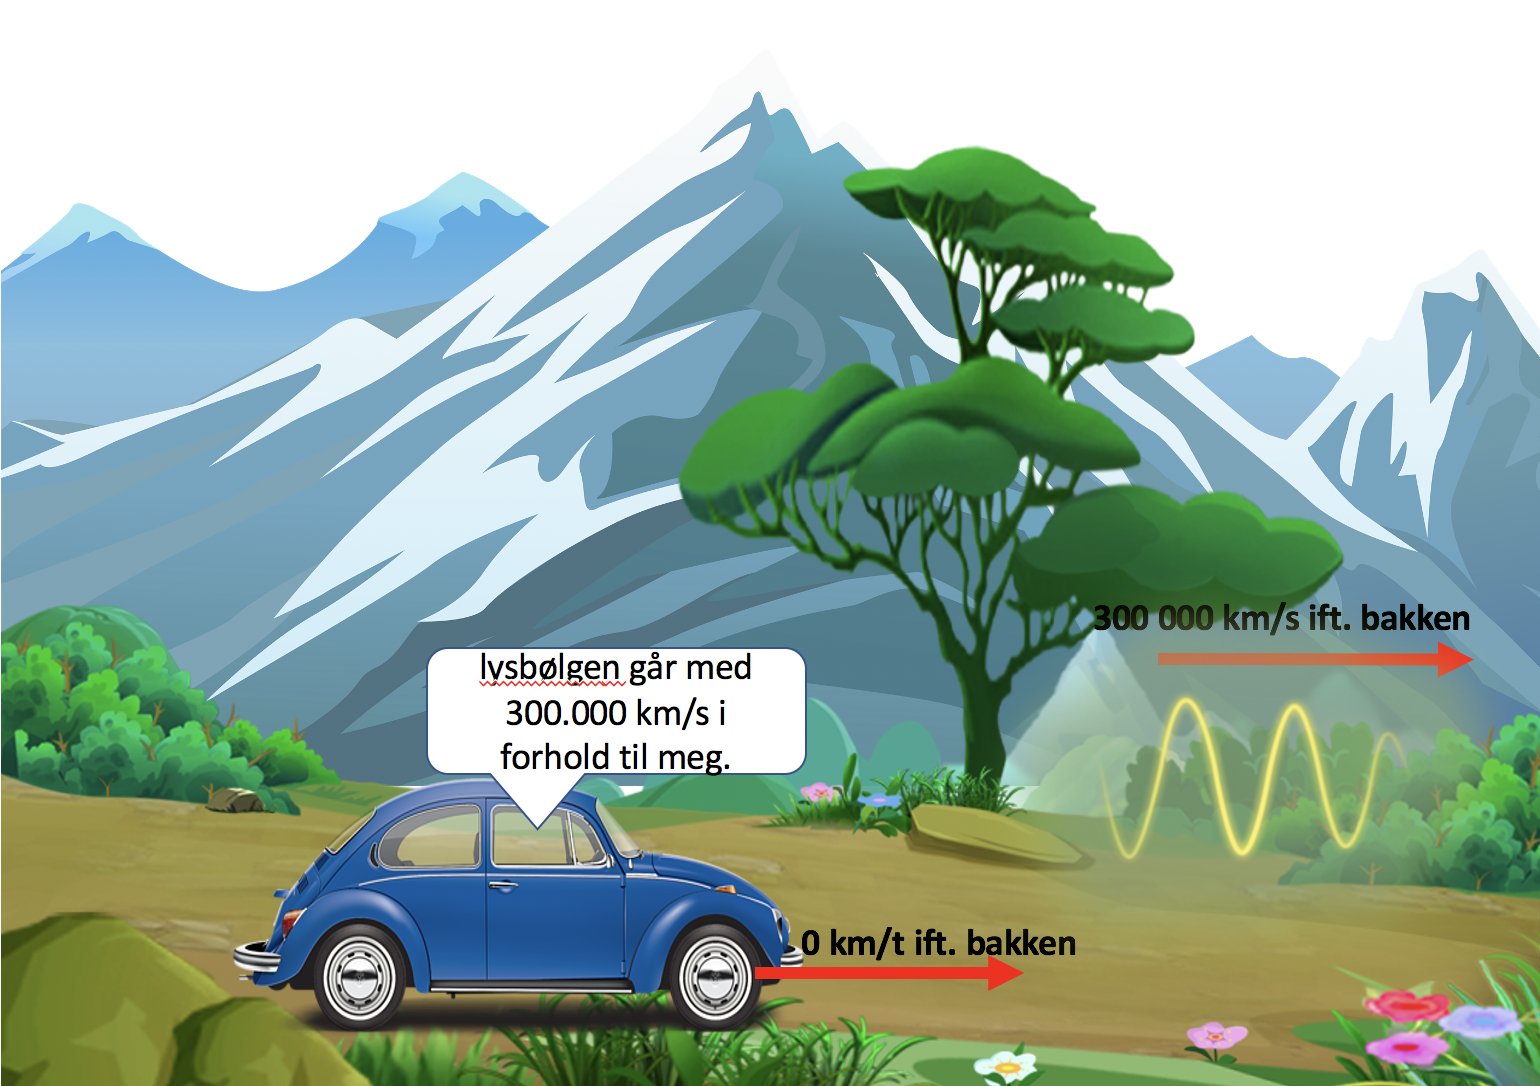
\includegraphics[scale=0.3]{media/klassrel8.png}}
La oss se på situasjonen med bilen men nå et foton eller lysbølge isteden for den oransje bilen.
}{SIDE 19/23/61}


\fullframe{kr12}{kr11}{kr13}{0}{\large
\centerline{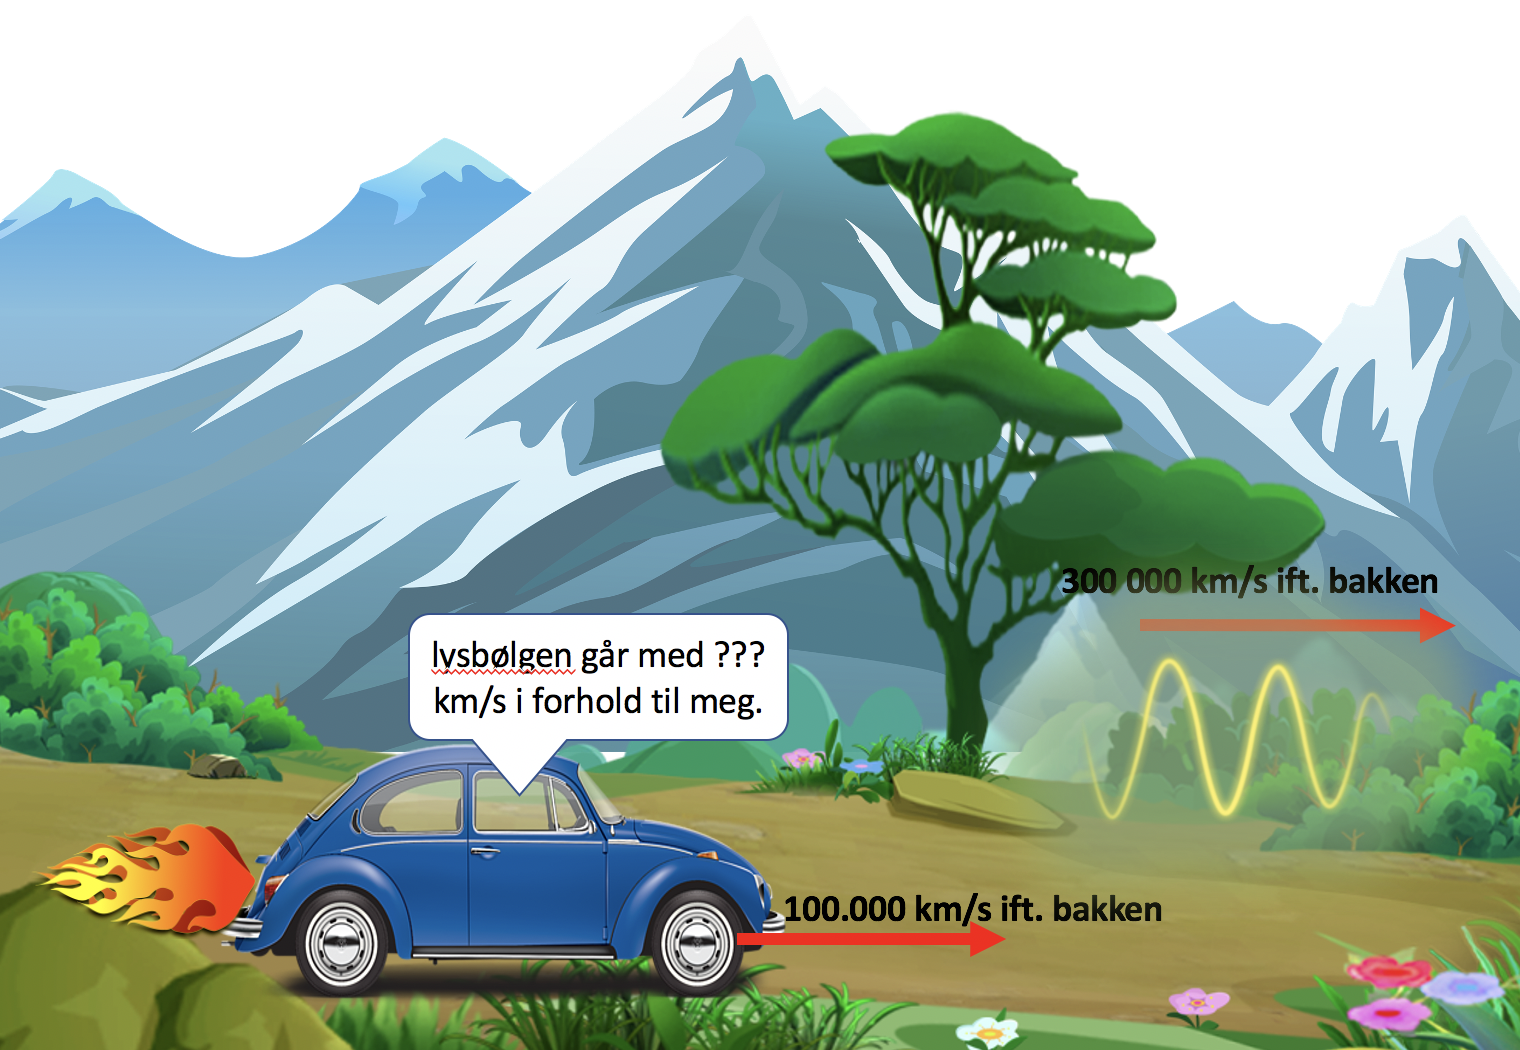
\includegraphics[scale=0.3]{media/klassrel9.png}}
Her har vi en superraskt bil som har nådd 1/3 av lyshastigheten. Men hvilken hastighet måler observatøren i bilen lyset til å ha?
}{SIDE 20/23/61}


\fullframe{kr13}{kr12}{kr14}{0}{\large
\centerline{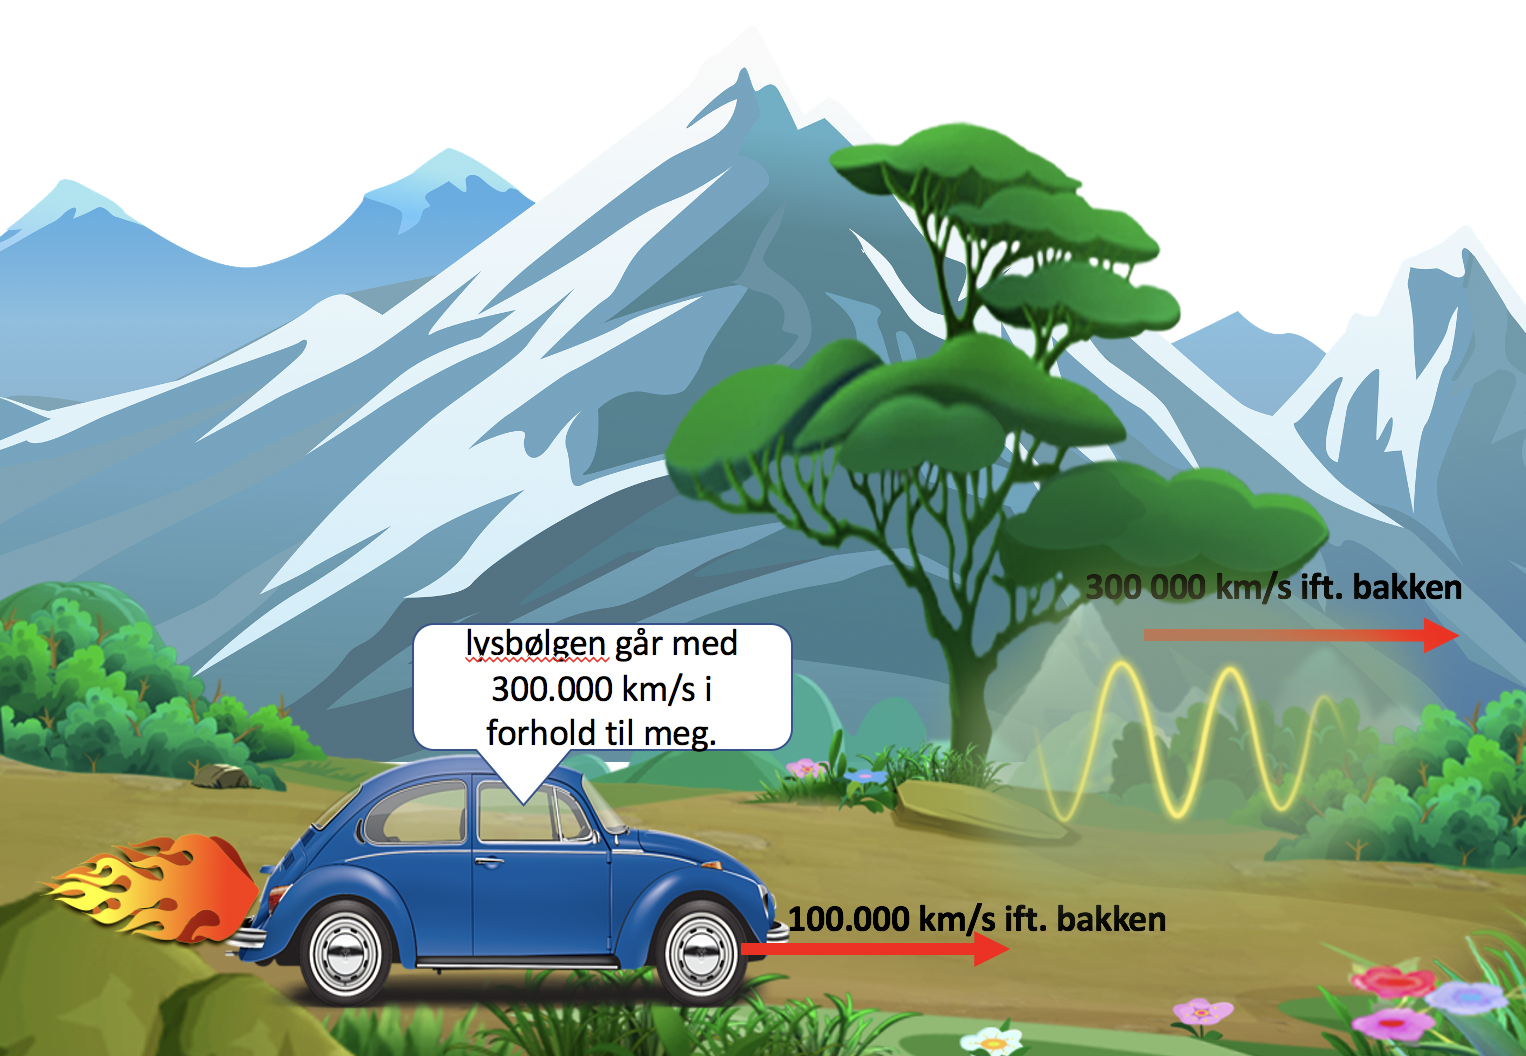
\includegraphics[scale=0.3]{media/klassrel10.png}}
Nettopp ja! Vi vet nå at hastigheten til lys er den samme målt fra alle referansesystemer, så da blir det vel slik?
}{SIDE 21/23/61}

\fullframe{kr14}{kr13}{kr15}{0}{
\centerline{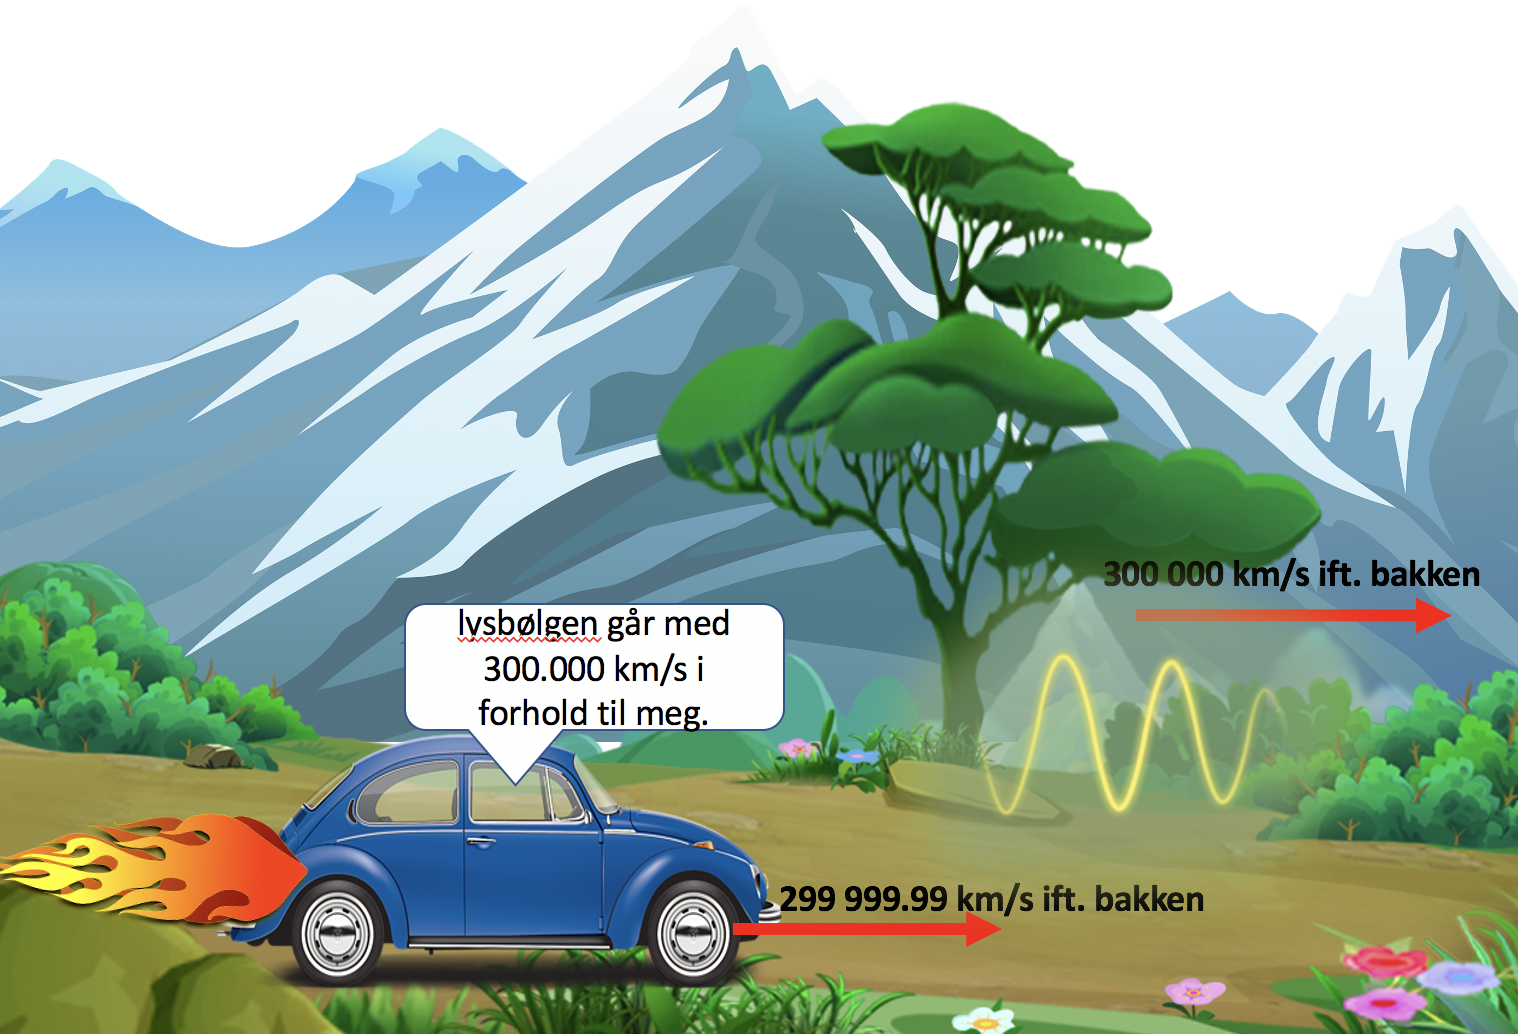
\includegraphics[scale=0.3]{media/klassrel11.png}}
{\bf Men nå begynner det vel å bli absurd??} Bilen har praktisk talt lyshastighet (den kan aldri få lyshastighet siden den har masse: det trengs uendelig med energi for å få noe som har masse til å nå lyshastighet. Fotoner er masseløse og kan derfor gå med lysets hastighet, dette kommer vi nærmere tilbake til). \textcolor{red}{Enda måler den lyset til å ha lyshastighet i forhold til seg selv?}
}{SIDE 22/23/61}

\fullframe{kr15}{kr14}{blue_nytema2}{0}{
\centerline{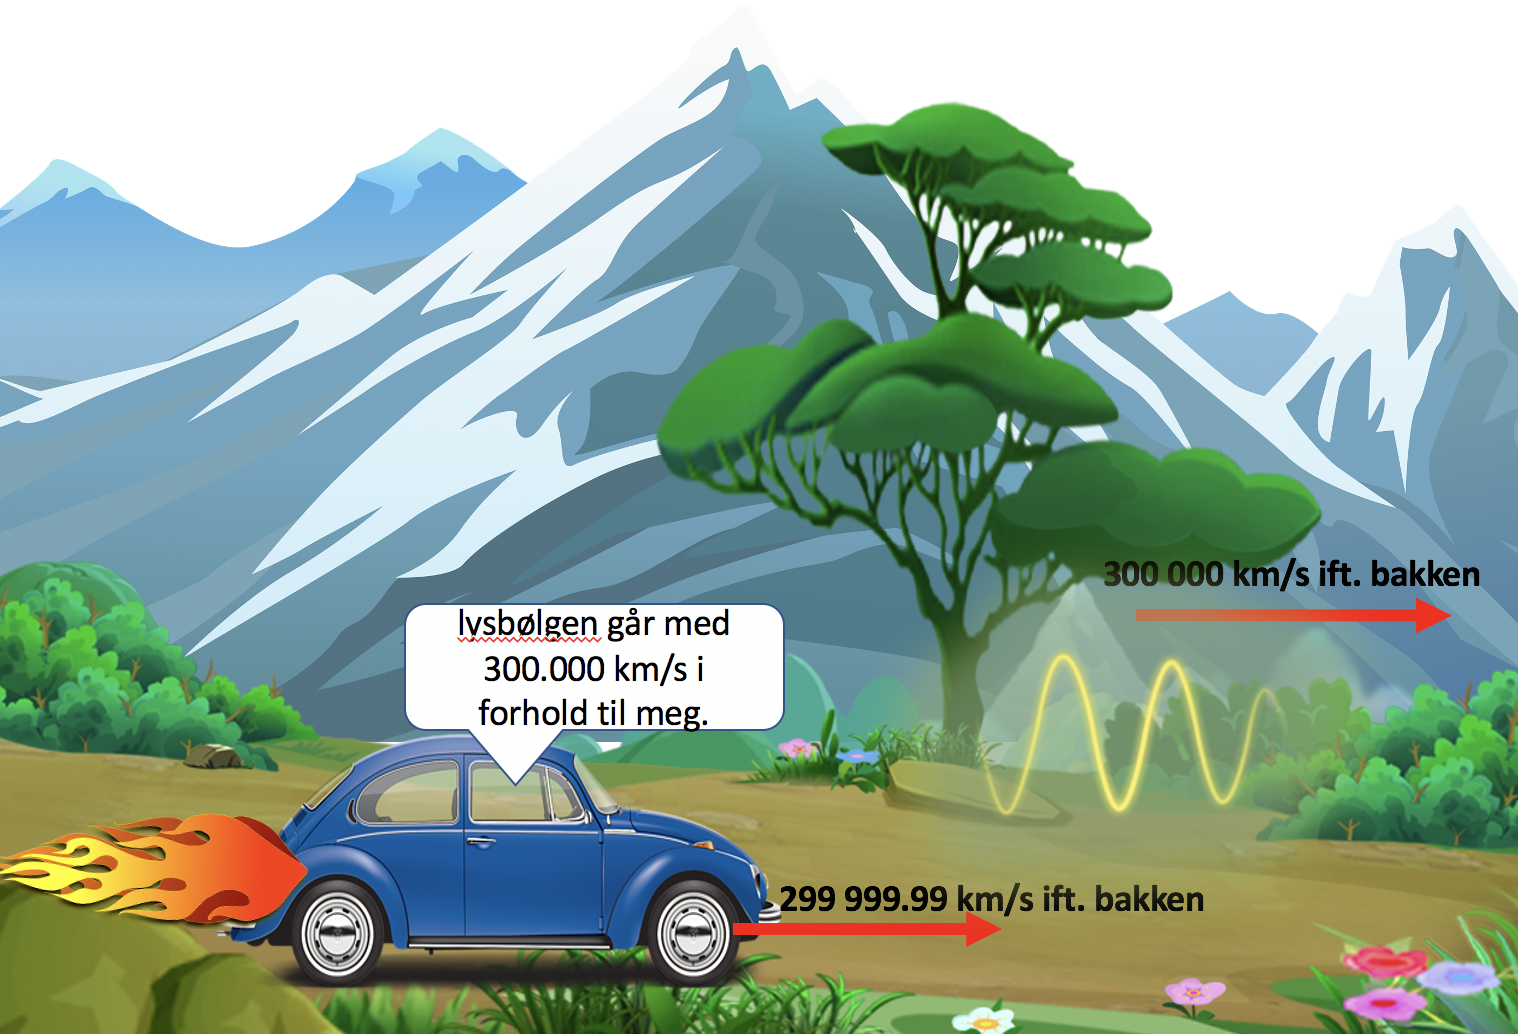
\includegraphics[scale=0.3]{media/klassrel11.png}}
Nettopp disse absurditetene var det Einstein ville se nærmere på for å få en bedre forståelse for det som skjer. Han oppdaget raskt at vi da fikk selvmotsigelser. Einstein utledet relativitetsteorien basert på disse selvmotsigelsene. Vi skal nå følge et av Einsteins egne tankeeksperimenter. Et av de som satte ham på sporet av relativitetsteorien...
}{SIDE 23/23/61}


\renewcommand{\headline}{Et tankeeksperiment}
{
\setbeamercolor{background canvas}{bg=blue}
\begin{frame}
\label{blue_nytema2}
\hyperlink{kr15}{\pagebutton{\small Forrige side}}
\nytemaside{0}
En strekk på bena, og kanskje en klementin? Er jo tida for det nå! (men pepperkakene må du vente med!)
Vi skal ta en pause halvveis ut i dette lange tankeeksperimentet.
\hyperlink{tog1}{\pagebutton{La oss bli med inn i Einsteins tankeverden...}}
\end{frame}
}


\fullframe{tog1}{kr15}{tog2}{0}{\label{tog}
\large
I det følgende skal vi se på og regne på et tankeeksperiment. La oss først innføre et begrep til: {\bf et event}. Dette er jo det engelske ordet for hendelse, likevel er det så godt innarbeidet som begrep i relativitetsteorien at vi beholder det engelske ordet her. Et event er rett og slett et punkt i tid og rom, akkurat som en hendelse jo er. Rett og slett et 4-dimensjonalt koordinat, en 3-dimensjonal posisjon og et tidspunkt for hendelsen.
}{SIDE 24/61/61}

\fullframe{tog2}{tog1}{tog3}{0}{\footnotesize
\centerline{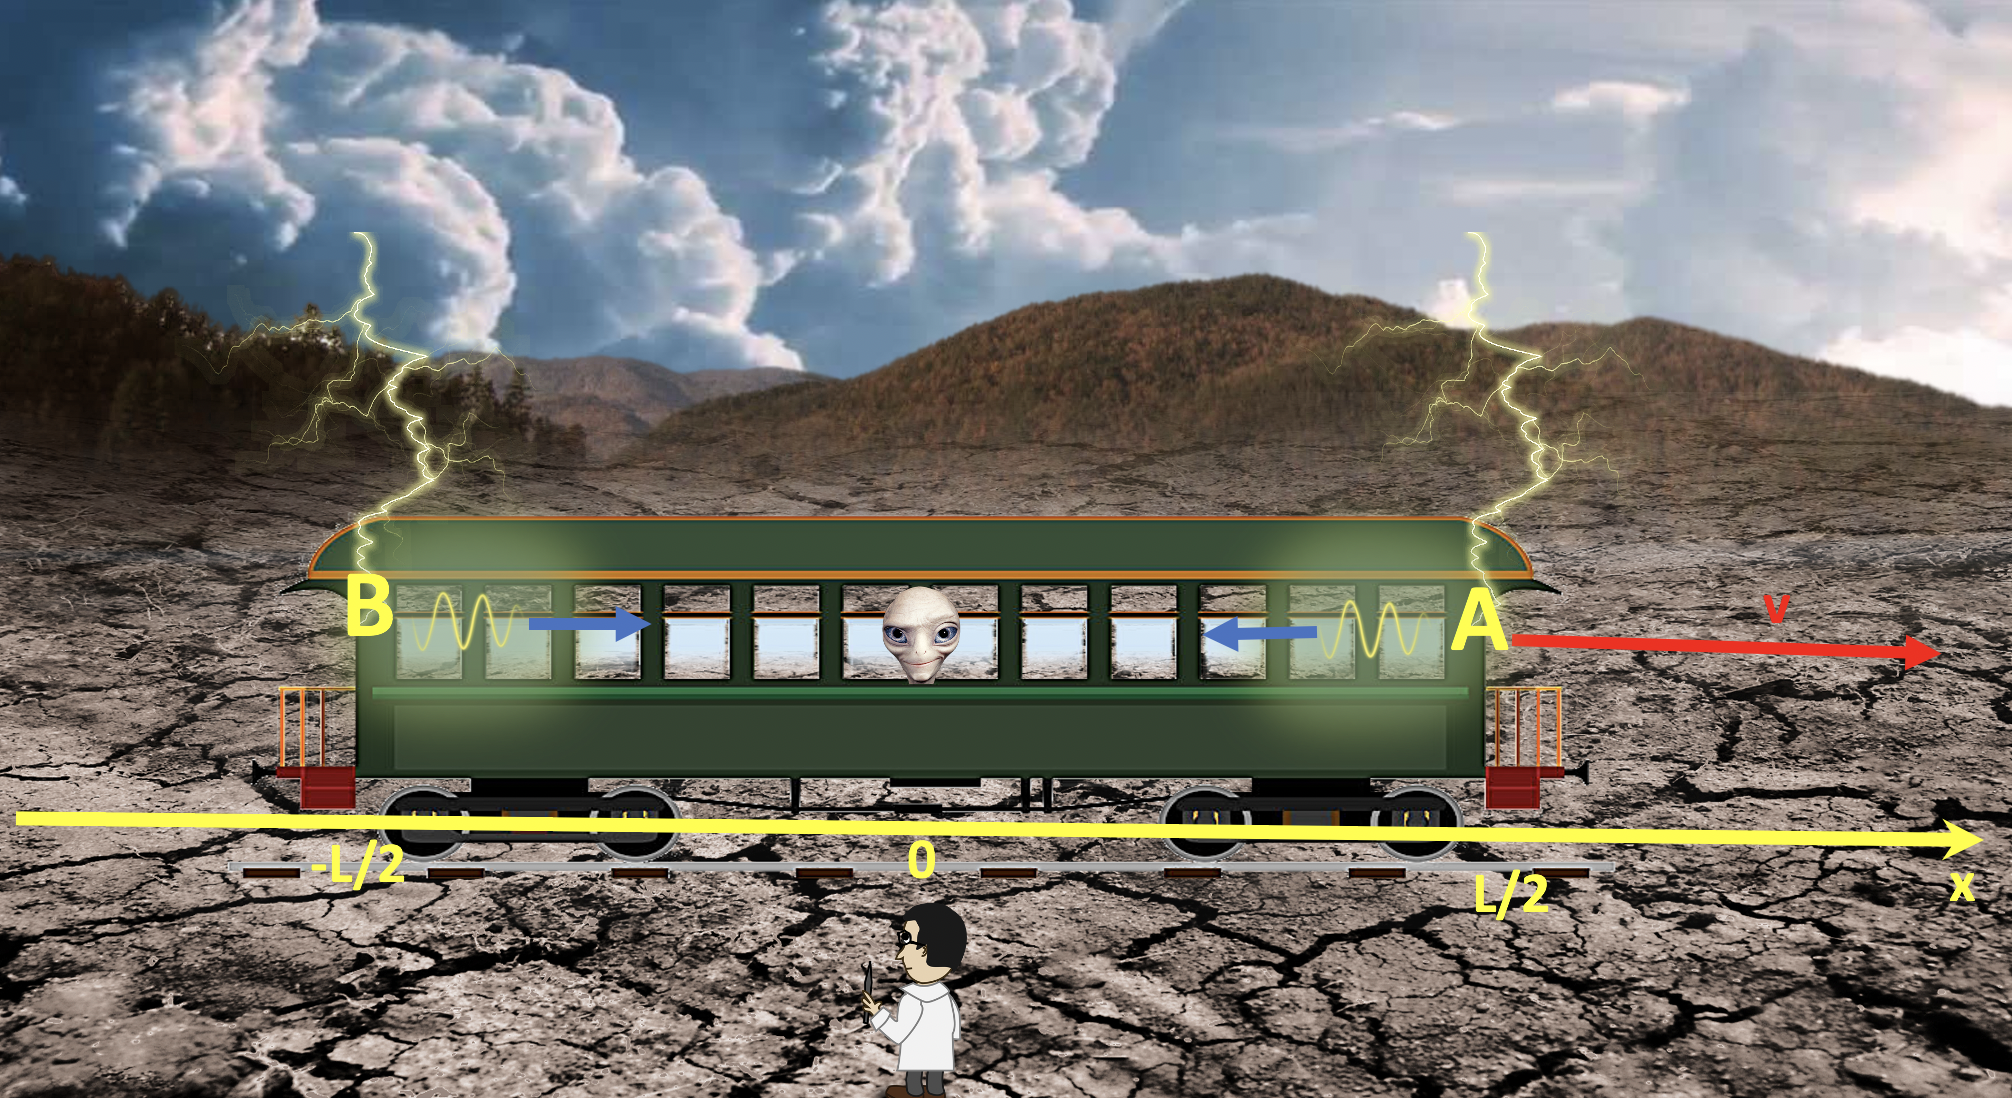
\includegraphics[scale=0.3]{media/tog1.png}}
Et tog ruller bortover mot høyre med fart $v$. Midt inne i toget har vi passasjer P med to store øyne. På bakken står professor O. Vi har en stor x-akse på bakken der professor O står i origo. Lengden av toget er $L$. På dette øyeblikksbildet er midten av toget, og dermed også passasjer P, i origo på x-aksen. Akkurat i dette øyeblikket slår to lyn ned samtidig, et foran i toget (event A) og et bak (event B). Lysstrålene fra de to lynnedslagene begynner å bre seg utover mot passasjer P (markert med lysbølger og blå piler)
}{SIDE 25/61/61}


\fullframe{tog3}{tog2}{tog3b}{0}{\footnotesize
\centerline{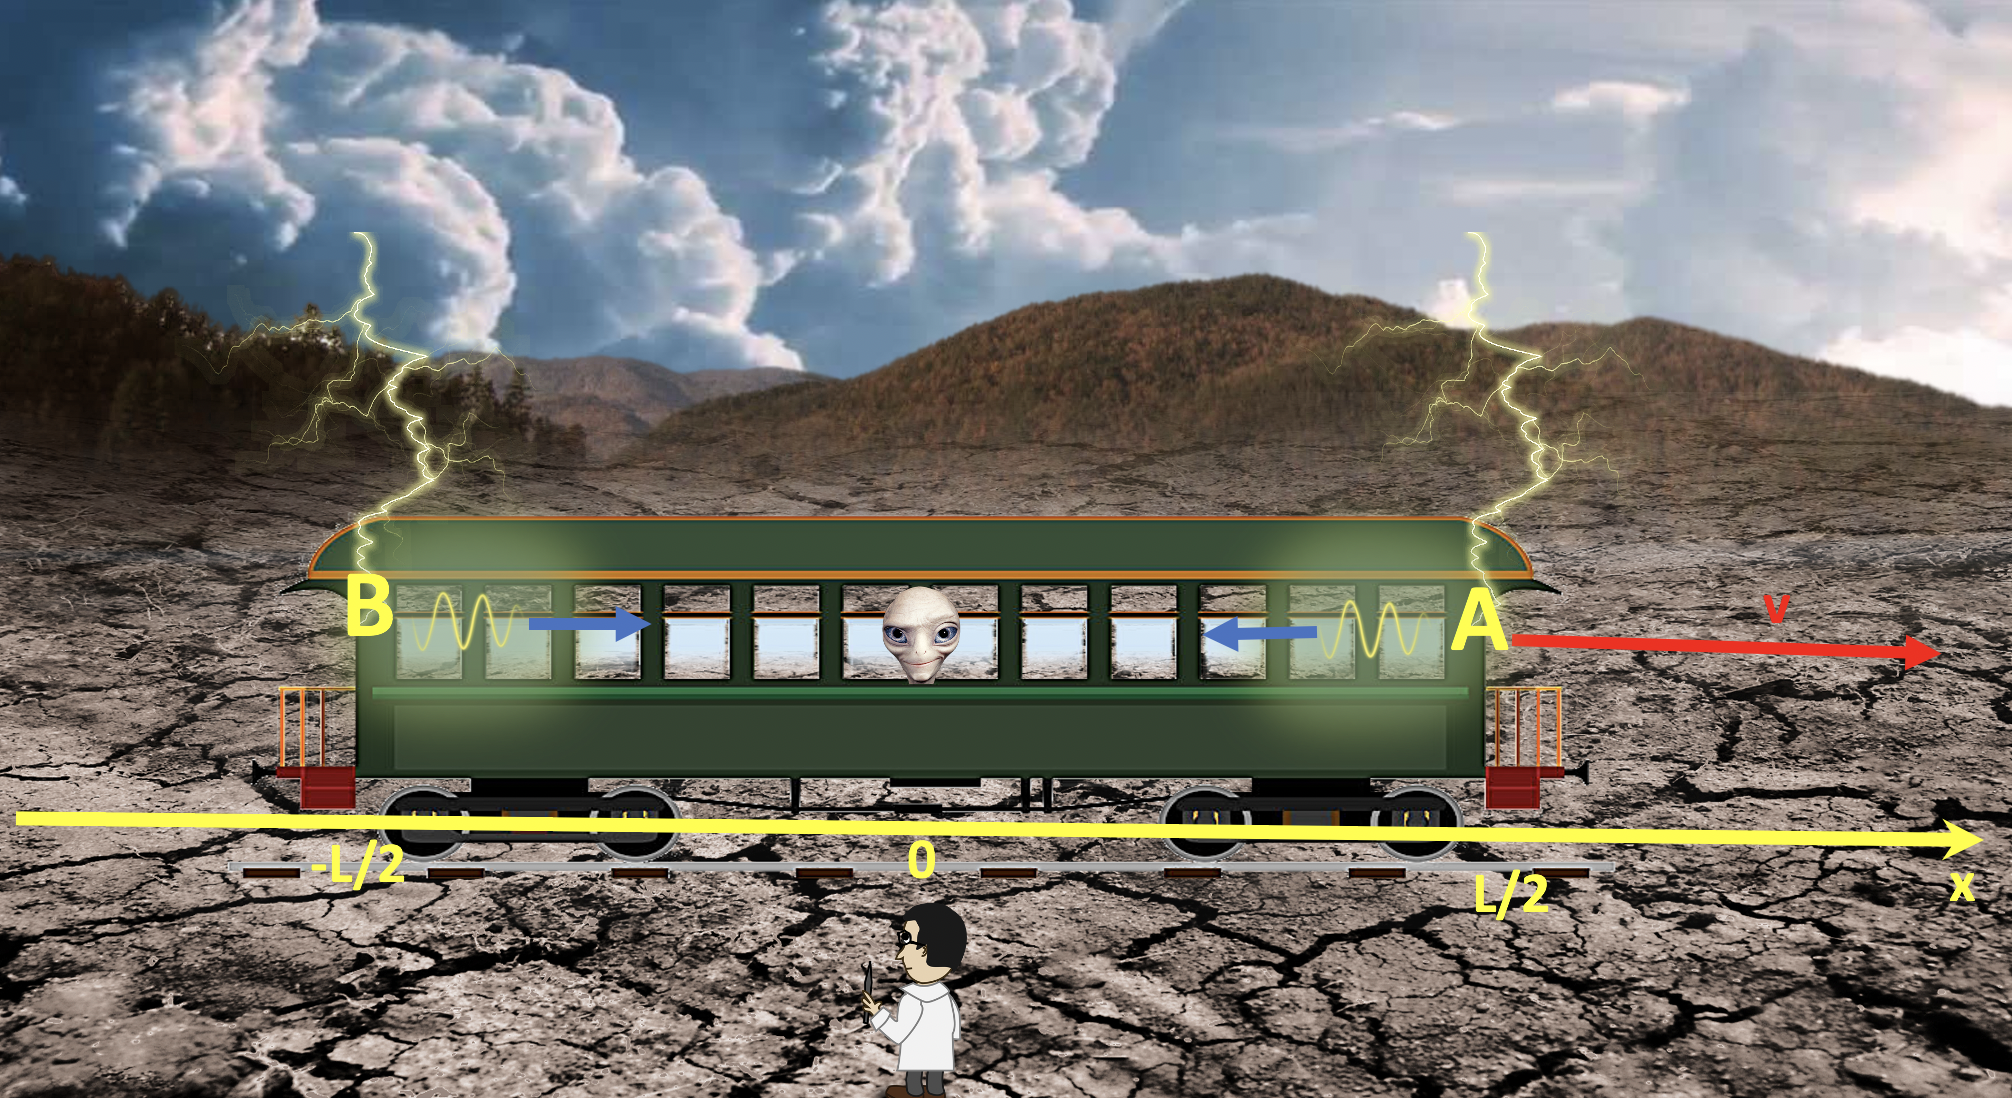
\includegraphics[scale=0.26]{media/tog1.png}}
Vi skal enda anta at vi ikke vet noe om Einsteins relativitetsteori. Vi skal nå prøve å tenke slik som Einstein gjorde før han hadde oppdaget relativitetsteorien. Når vi jobber med problemer i relativitetsteori, er det viktig å skrive ned posisjons- og tidskoordinater for eventer. Vi sier at i det dette øyeblikksbildet ble tatt så starter vi en stoppeklokke slik at $t=0$ i dette øyeblikket. Da blir koordinatene til event A og B som følger:
\[
x_A=L/2,\ \ \ \ t_A=0, \ \ \ \ x_B=-L/2,\ \ \ \ t_B=0
\]
{\bf Enig?}
}{SIDE 26/61/61}

\fullframe{tog3b}{tog3}{tog3c}{0}{\footnotesize
\centerline{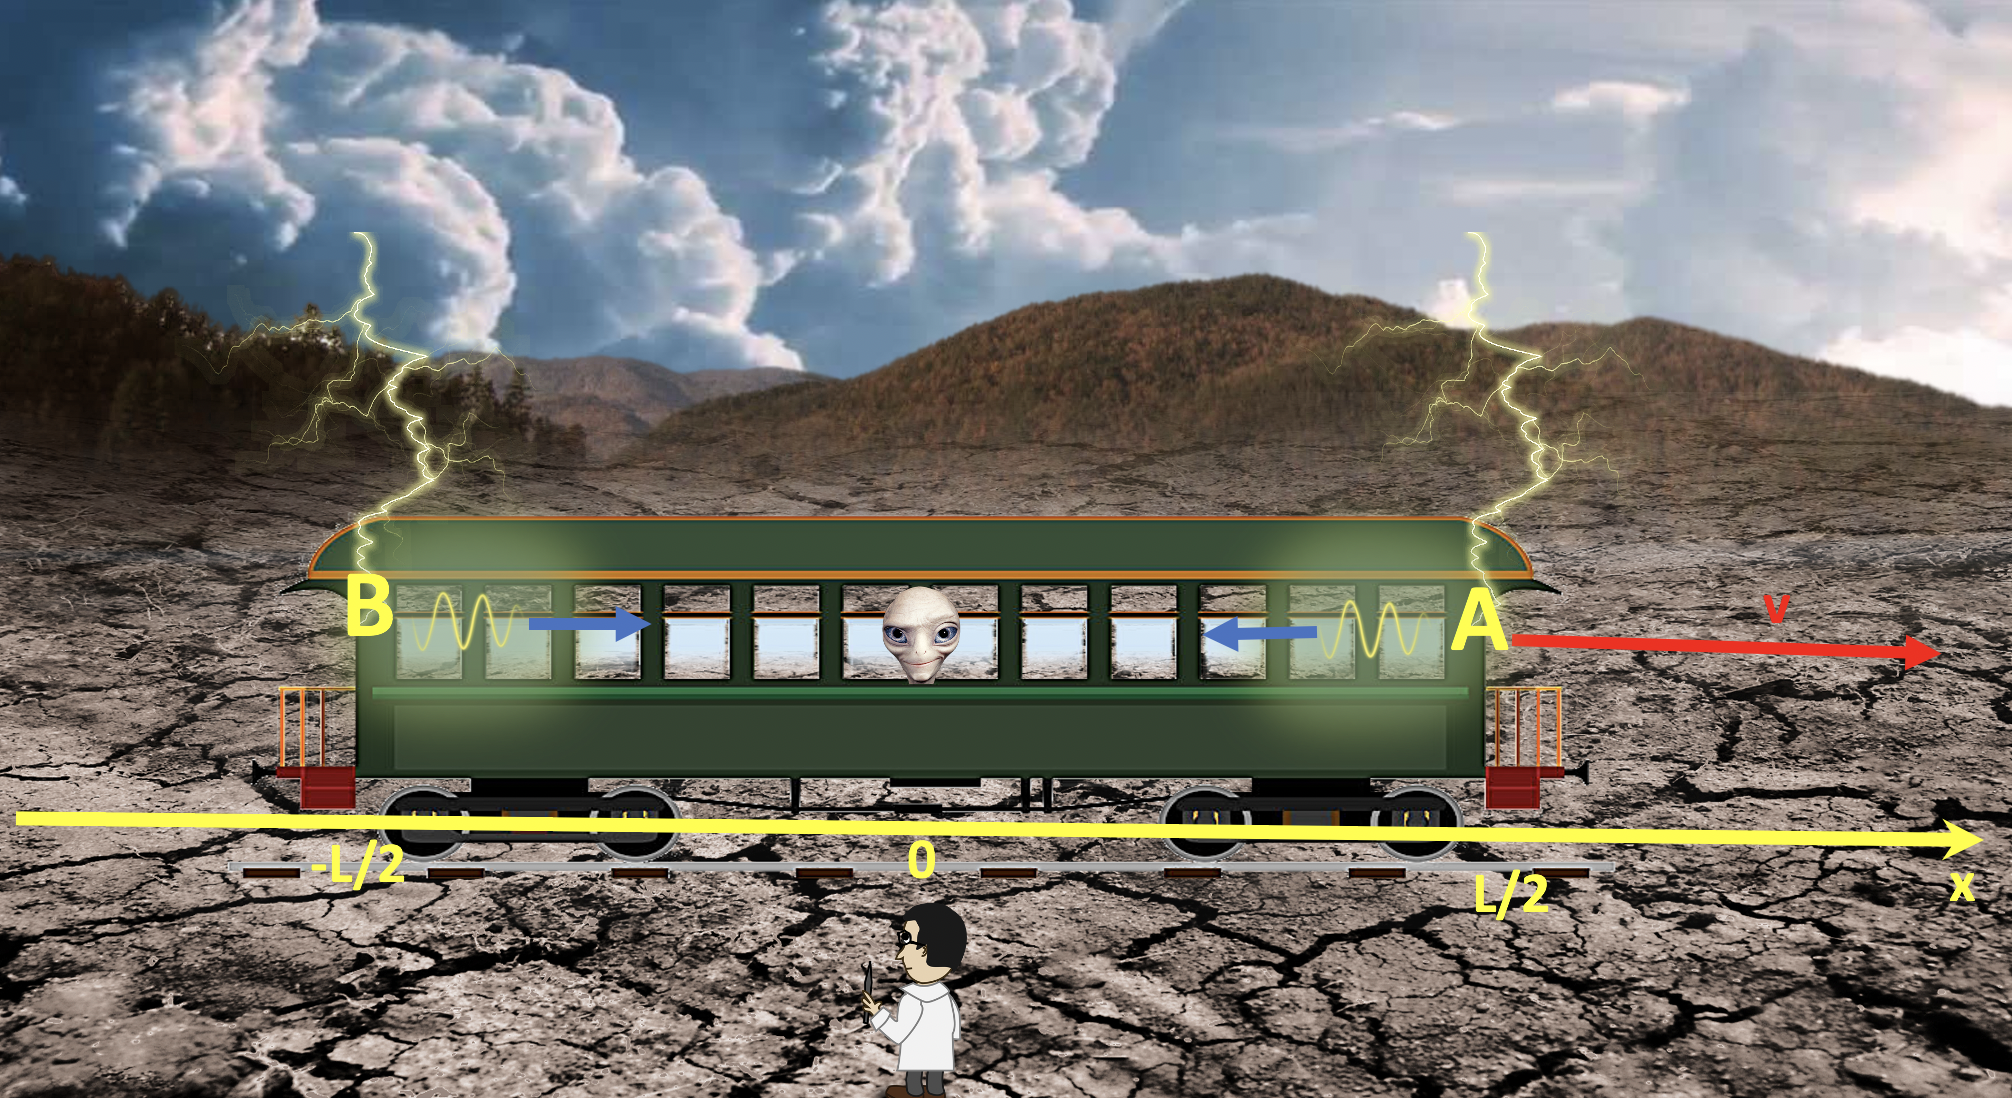
\includegraphics[scale=0.26]{media/tog1.png}}
Vi skal innføre et event til her, nemlig event P som er at professoren og passasjeren har samme x-koordinat (vi regner kun på x-posisjoner her siden all bevegelse er i x-retning, det er ingen bevegelse i y-retning). Det betyr at i dette øyeblikket så kan de to håndhilse og utveksle informasjon. Posisjon og koordinat til dette eventet må vel være:
\[
x_P=0,\ \ \ \ t_P=0
\]
{\bf Fortsatt enig?}
}{SIDE 27/61/61}

\fullframe{tog3c}{tog3b}{tog4}{0}{\footnotesize
\centerline{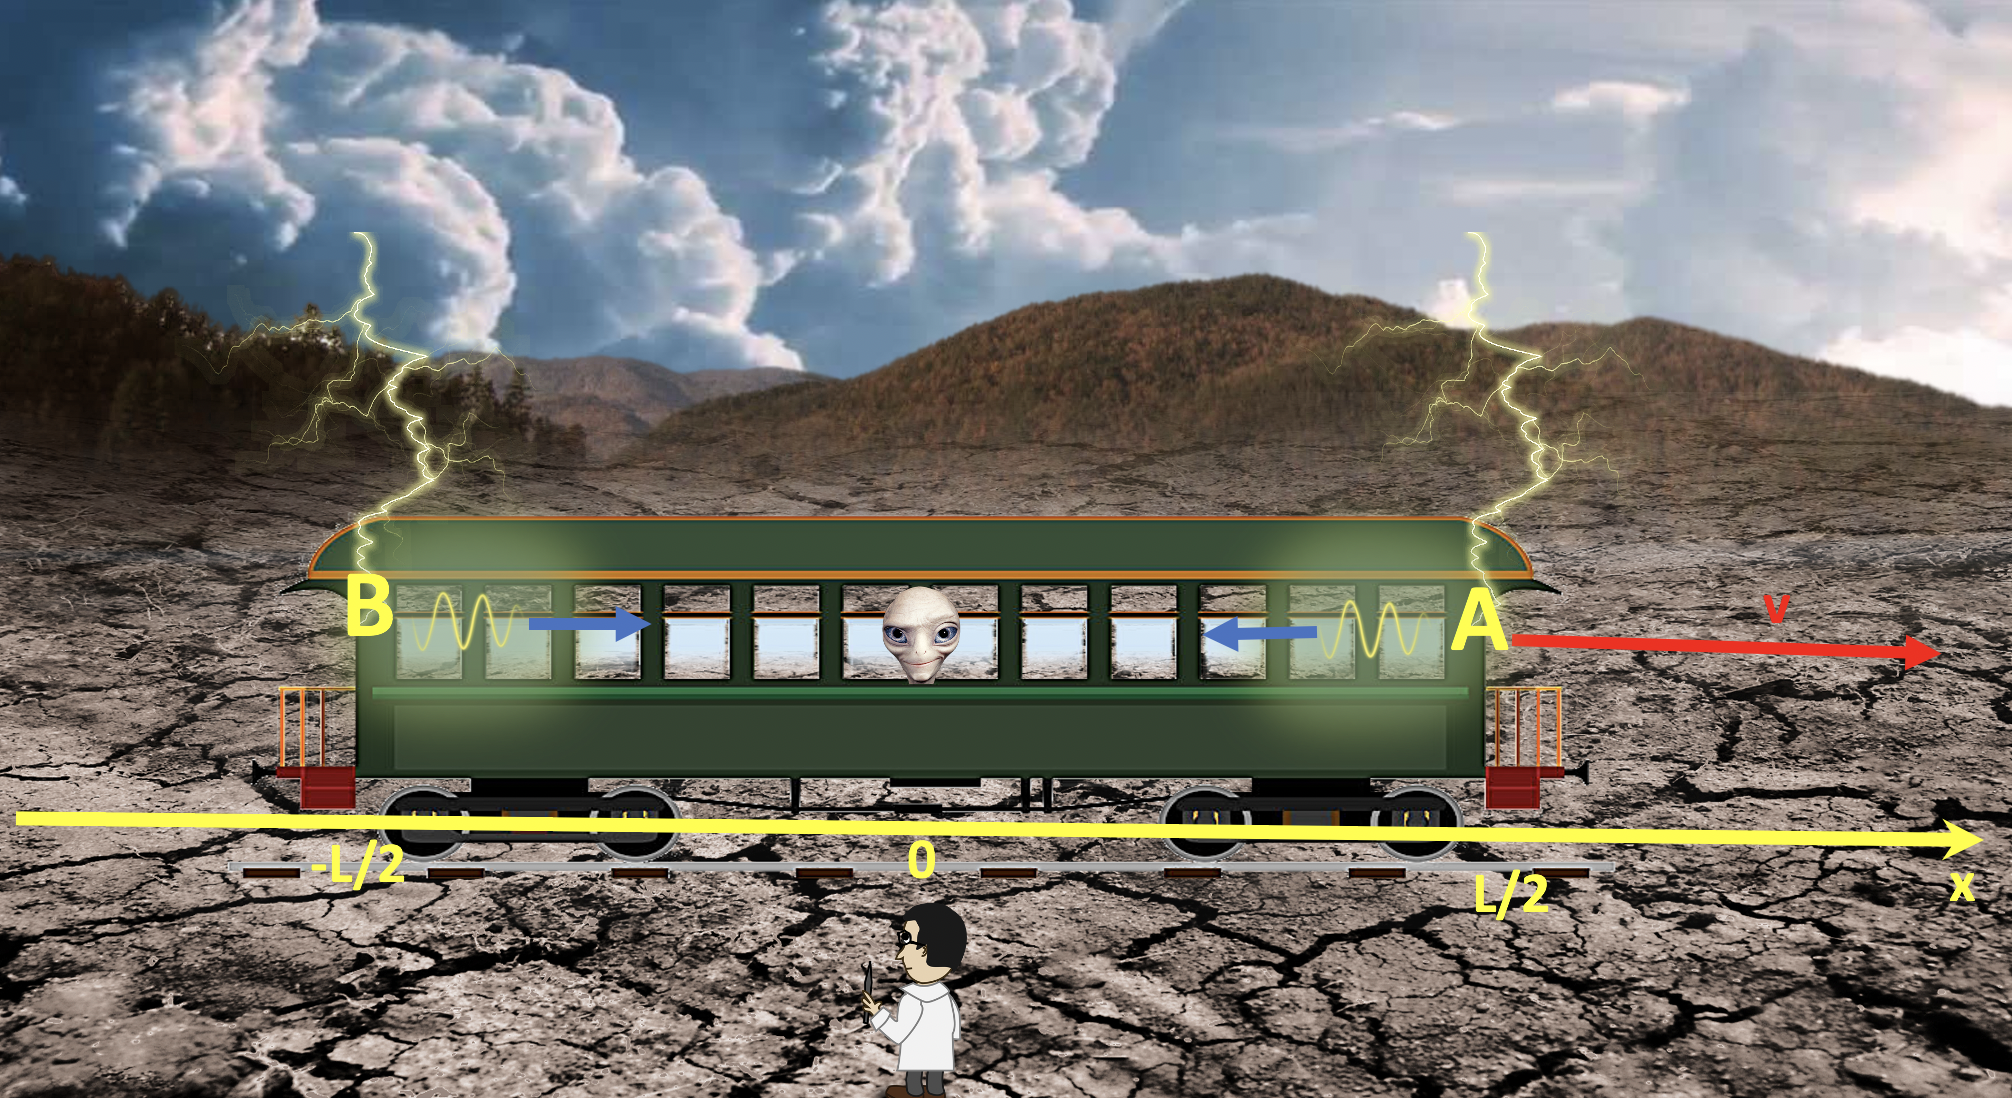
\includegraphics[scale=0.26]{media/tog1.png}}
Er du også enig i at professoren vil se lysglimtene fra de to lynnedslagene samtidig? Professoren står på bakken i en avstand $L/2$ fra både event A og B. De to eventene er samtidige, lyset går med samme fart fra begge lynnedslagene, dermed vil professoren se at lynnedslagene er samtidige. Men hva med passasjer P?
}{SIDE 28/61/61}

\choiceframe{tog4}{tog3c}{0}{\footnotesize
\centerline{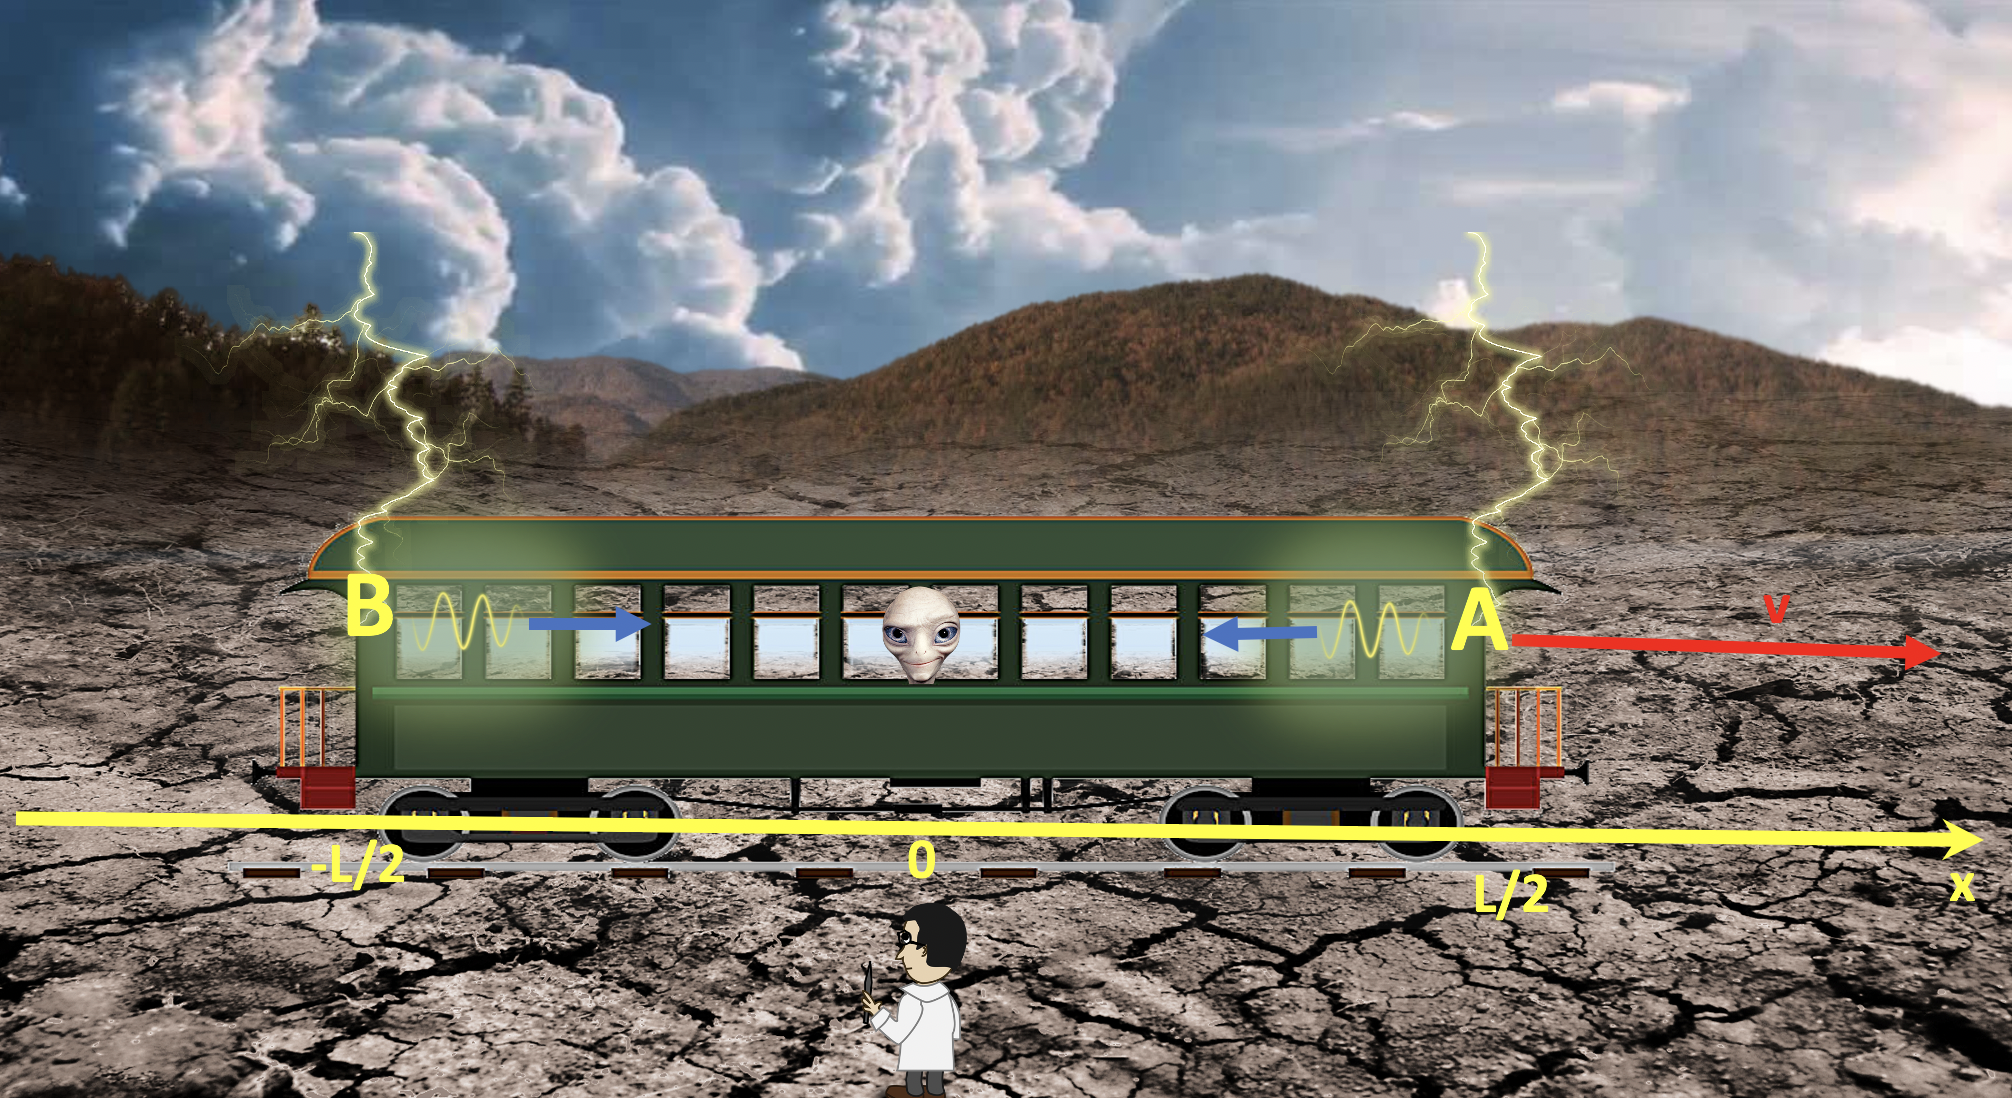
\includegraphics[scale=0.26]{media/tog1.png}}
Tenk på hvordan toget beveger seg, passasjeren beveger seg og lysbølgene fra lynnedslagene. Hva vil passasjer P se?
\hyperlink{feil_tog4a}{\choicebutton{P ser begge samtidig}}\hyperlink{riktig_tog4b}{\choicebutton{P ser A før B}}\hyperlink{feil_tog4a}{\choicebutton{P ser B før A}}
}{SIDE 29/61/61}

\colchoiceframe{feil_tog4a}{tog4}{0}{black}{\large
\textcolor{yellow}{Neeeei, ikke helt! Hvordan beveger passasjer P seg i forhold til hver av lysstrålene? Går en av lysstrålene fortere enn den andre eller går de like fort? (hint: dette er lys!)}
}{SIDE 30/61/61}

\colfullframetxt{riktig_tog4b}{tog4}{tog5}{-1}{yellow}{Ok, slik må det være!}{
\centerline{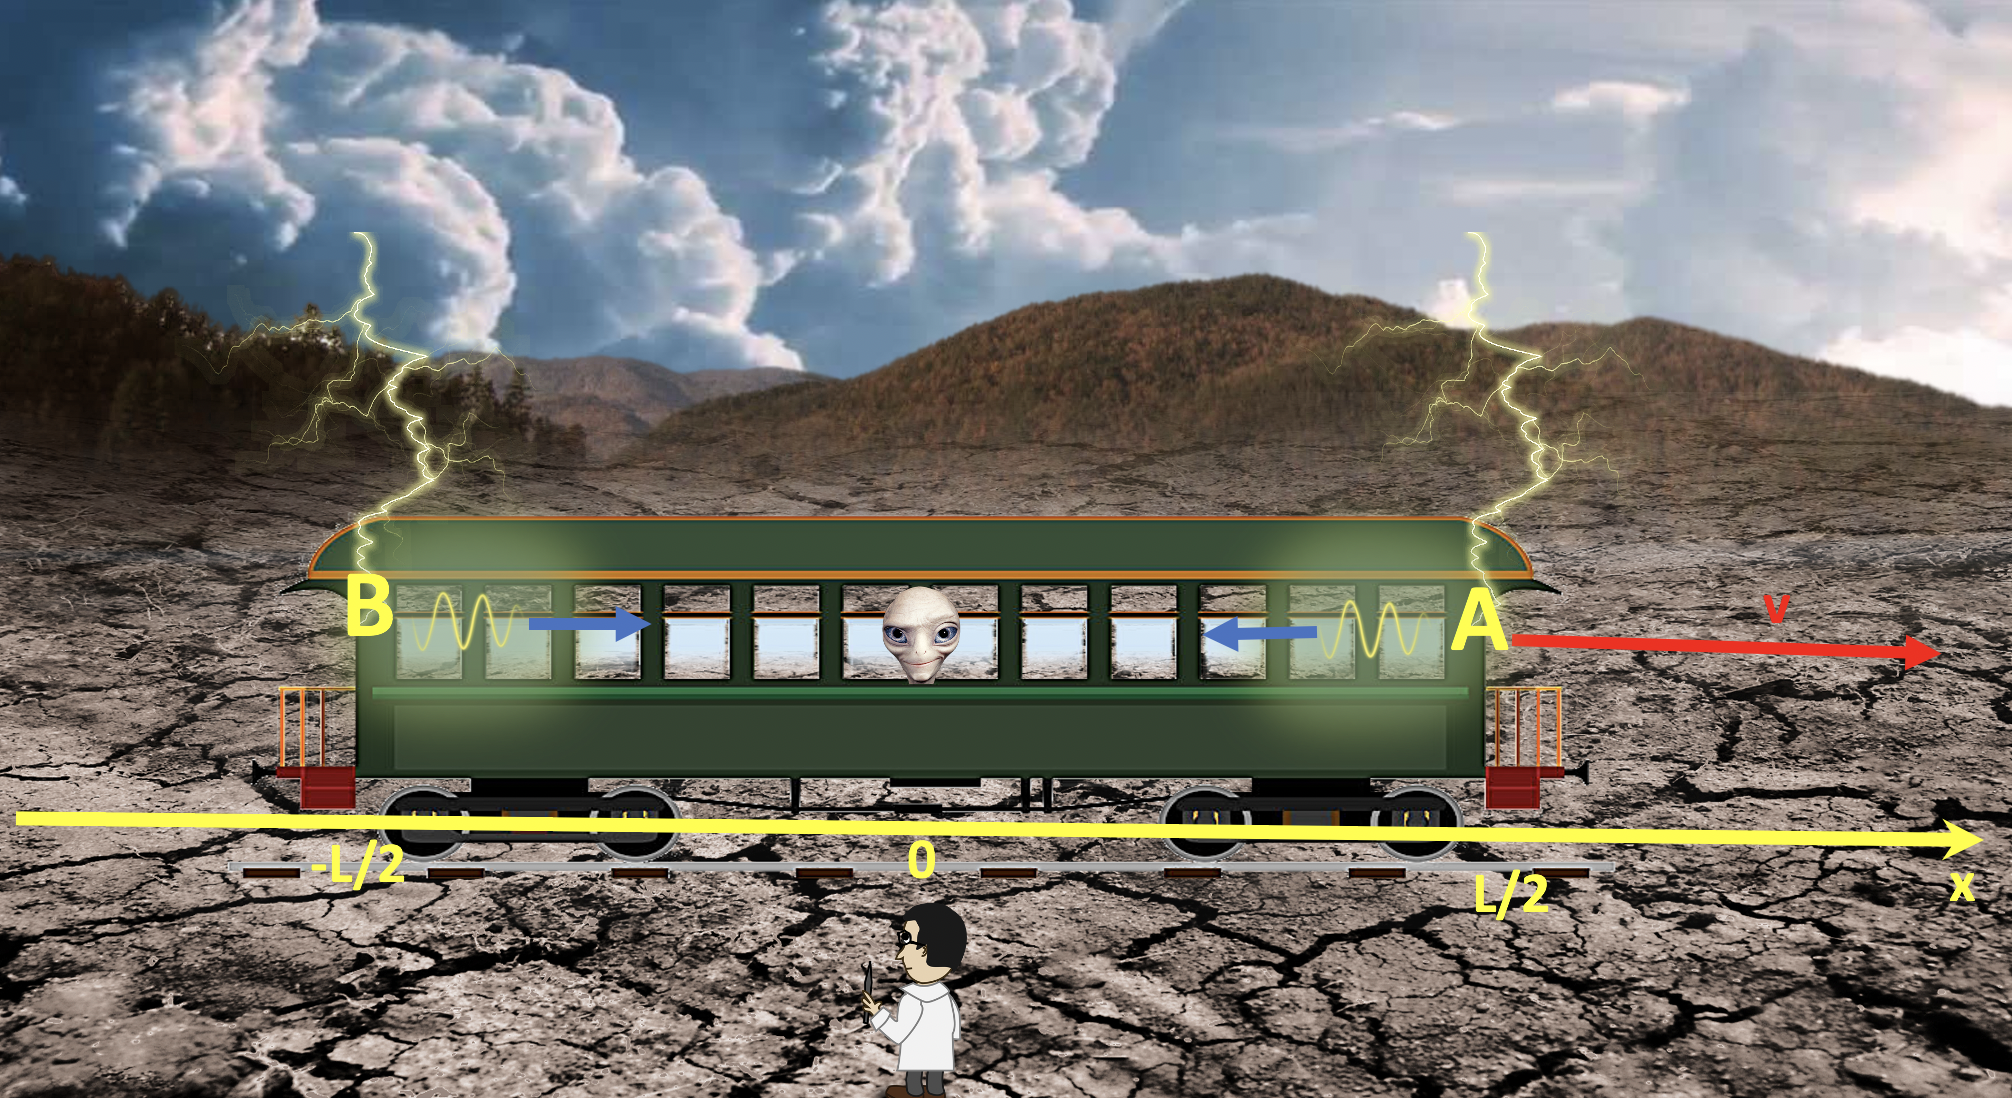
\includegraphics[scale=0.26]{media/tog1.png}}
Det stemmer. Må det ikke bli slik da: toget (og dermed passasjer P) beveger seg {\bf mot} lysstrålen fra A men vekk fra lysstrålen fra B. Vi har lært at lys alltid går med lyshastighet uansett referansesystem, så lysstrålene går like fort. Men hvis passasjeren da beveger seg mot lysstrålen fra A så vil vel den treffe passasjeren sitt ansikt først. Og siden passasjeren beveger seg vekk fra B, vil B treffe øynene til P senere? Og dermed må vel passasjeren se A for B?
}{SIDE 31/61/61}

\fullframe{tog5}{riktig_tog4b}{tog6}{0}{
\centerline{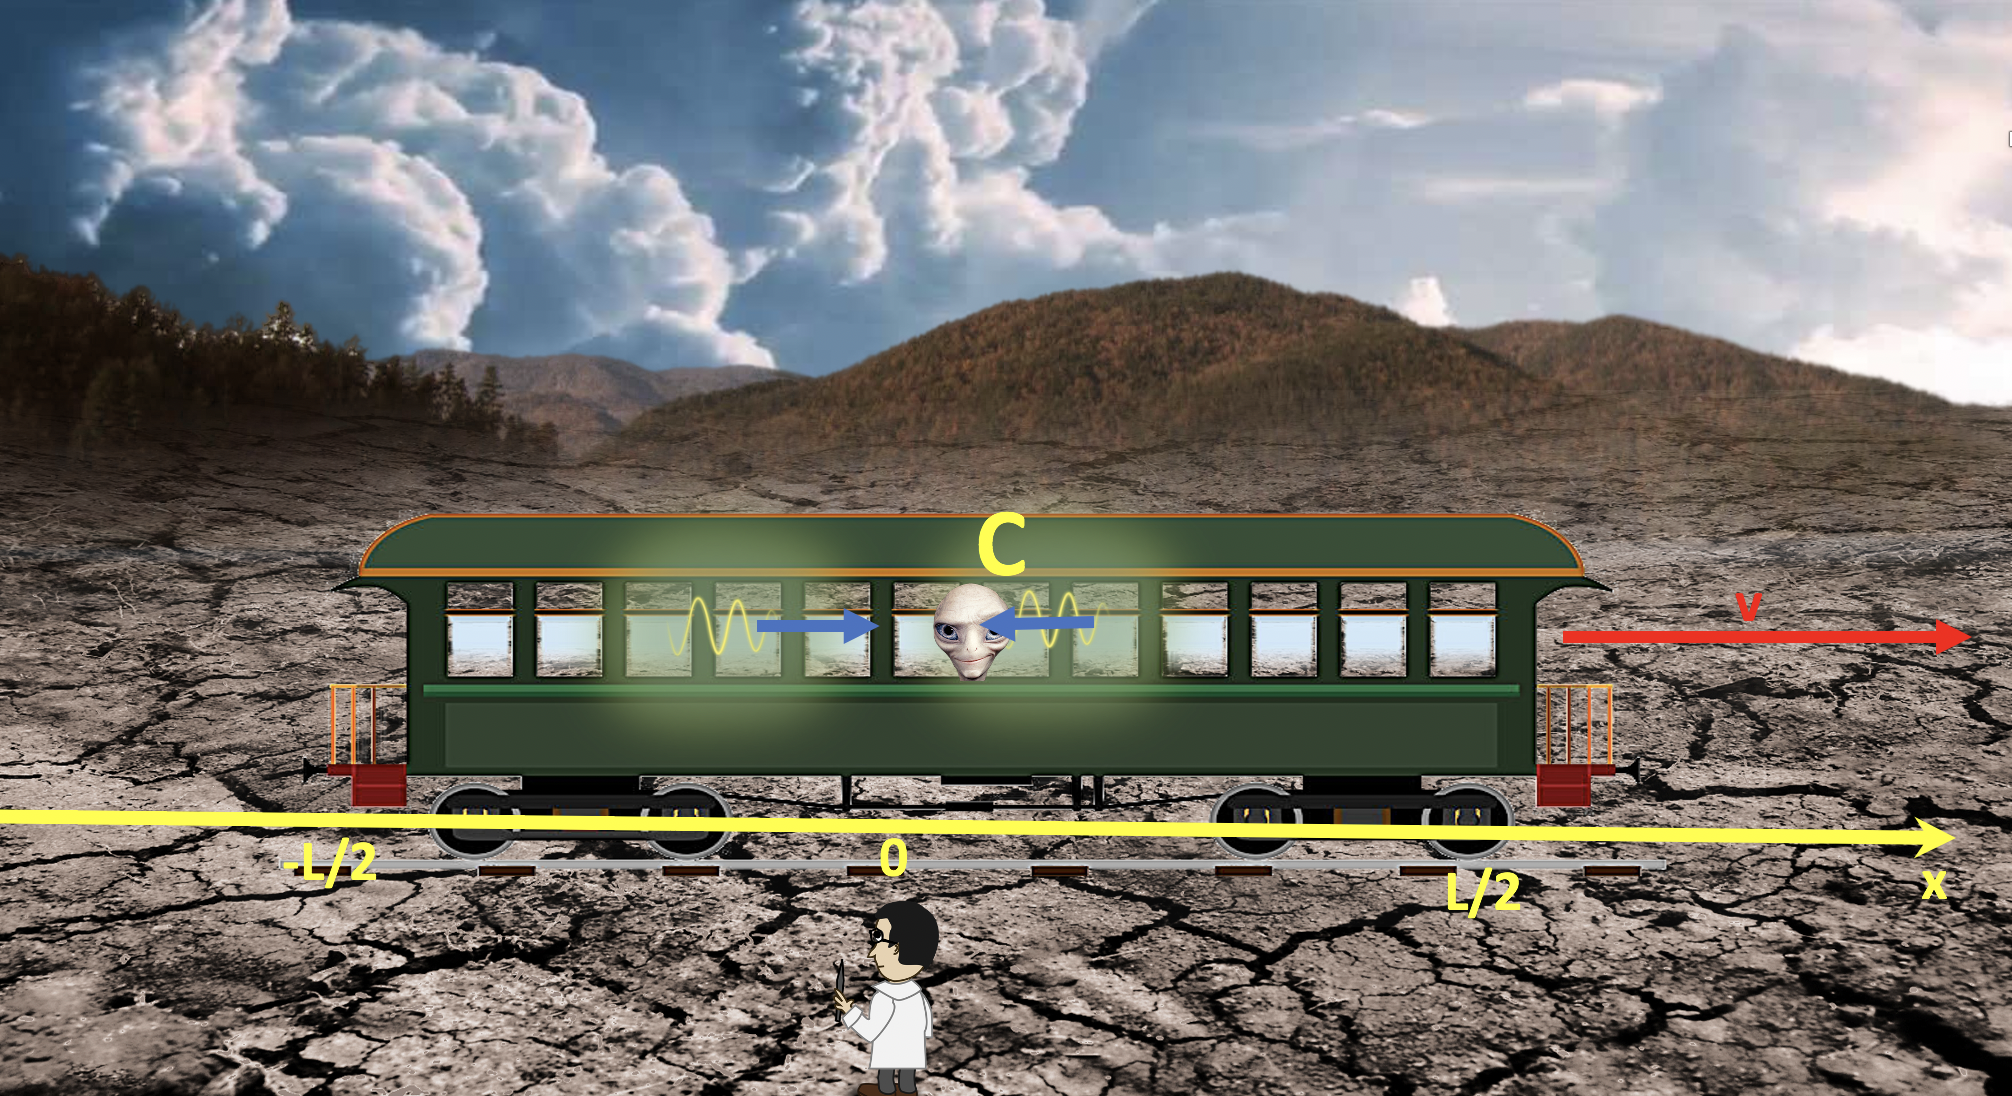
\includegraphics[scale=0.26]{media/tog2.png}}
Her ser vi {\bf event C} illustrert. Event C er når lysstrålen fra lynnedslag A treffer øyet til passasjer P slik at passasjeren ser at lynet har slått ned foran. Toget har beveget seg litt til høyre (med hastighet $v$), lysstrålen fra A her beveget seg mot venstre. Siden P har beveget seg bort fra lysstrålen fra B, så har denne lysstrålen enda ikke truffet og passasjer P vet dermed enda ikke at det skjedde et lynnedslag bak.
}{SIDE 32/61/61}


\fullframe{tog6}{tog5}{tog7}{0}{
\centerline{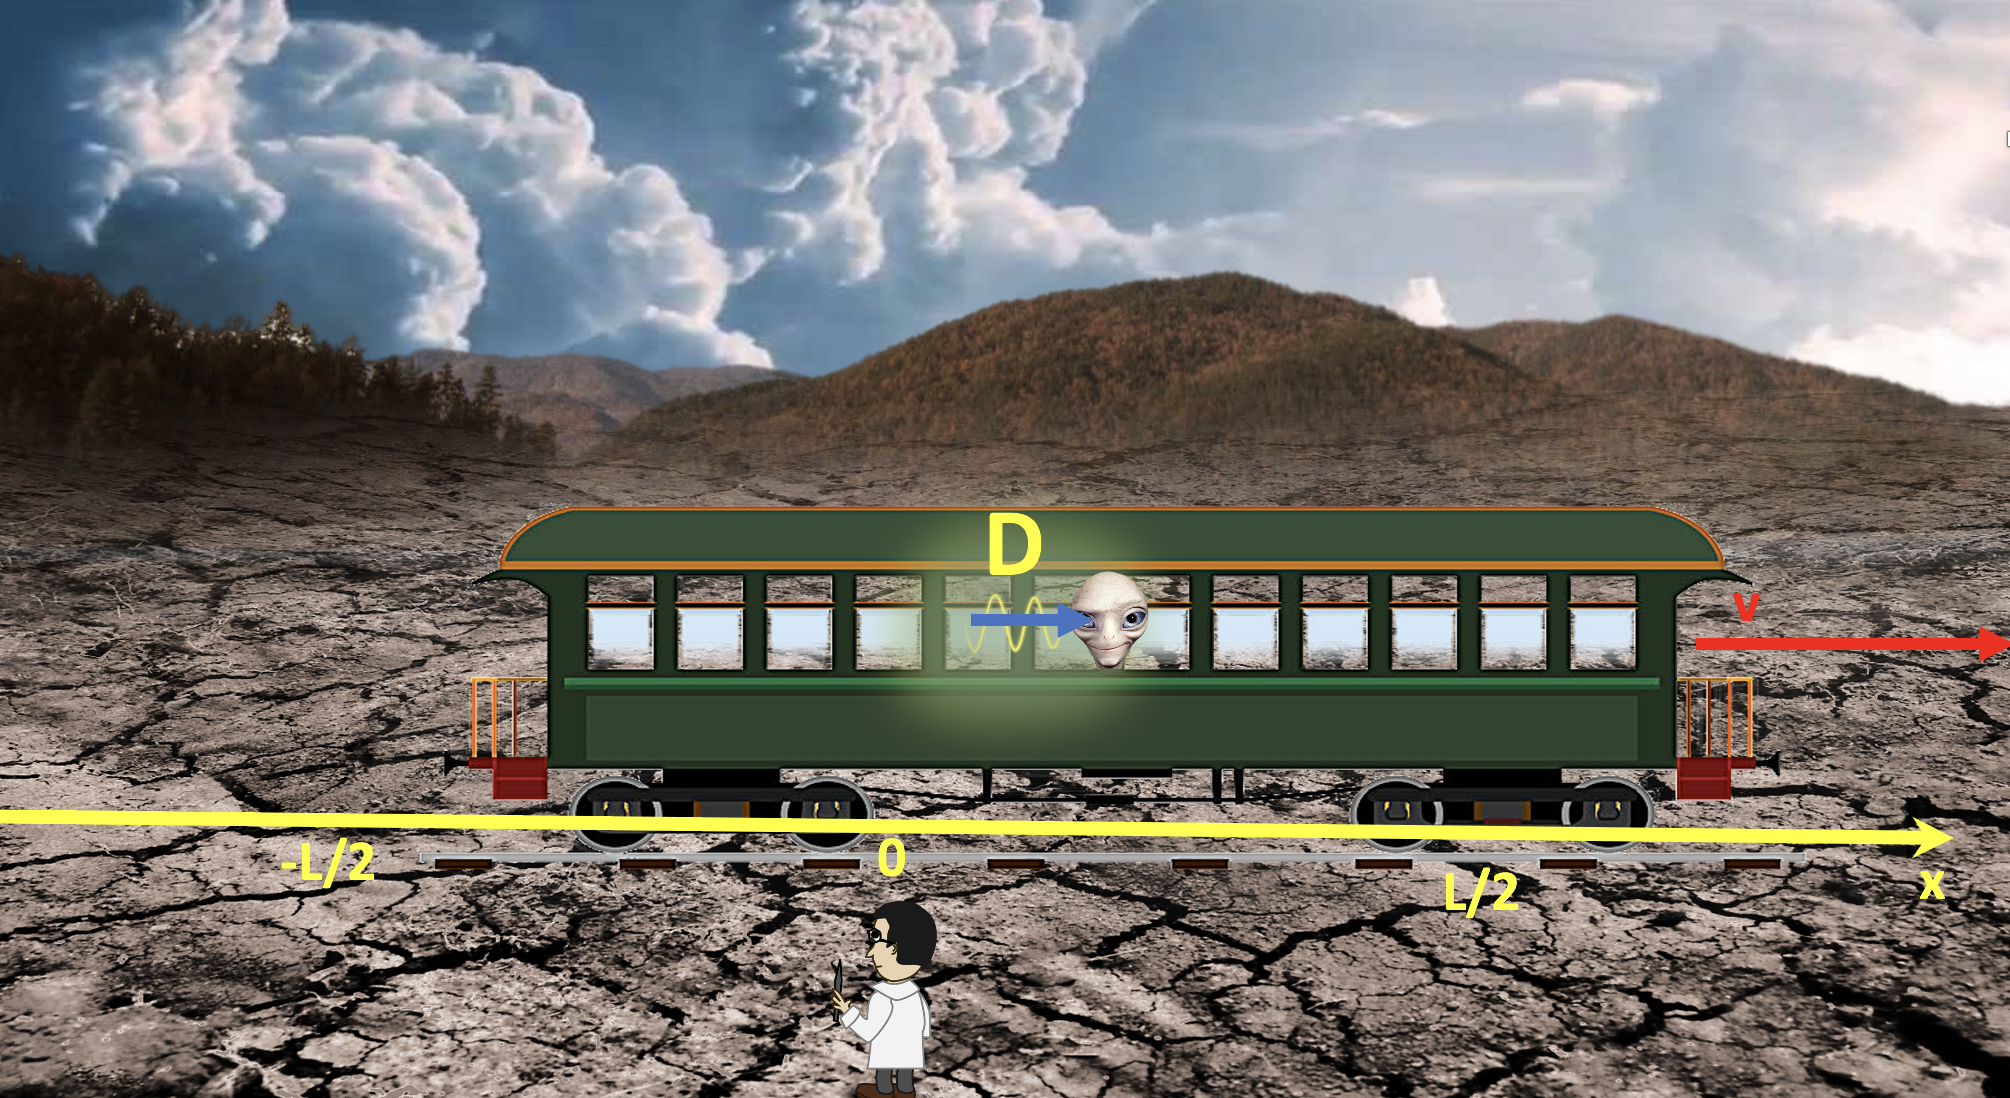
\includegraphics[scale=0.26]{media/tog3.png}}
Her ser vi {\bf event D} illustrert. Event D er når lysstrålen fra lynnedslag B treffer øyet til passasjer P slik at passasjeren ser at lynet har slått ned bak også. Toget har beveget seg enda litt lenger til høyre (med hastighet $v$).
}{SIDE 33/61/61}

\fullframe{tog7}{tog6}{tog8}{0}{
\centerline{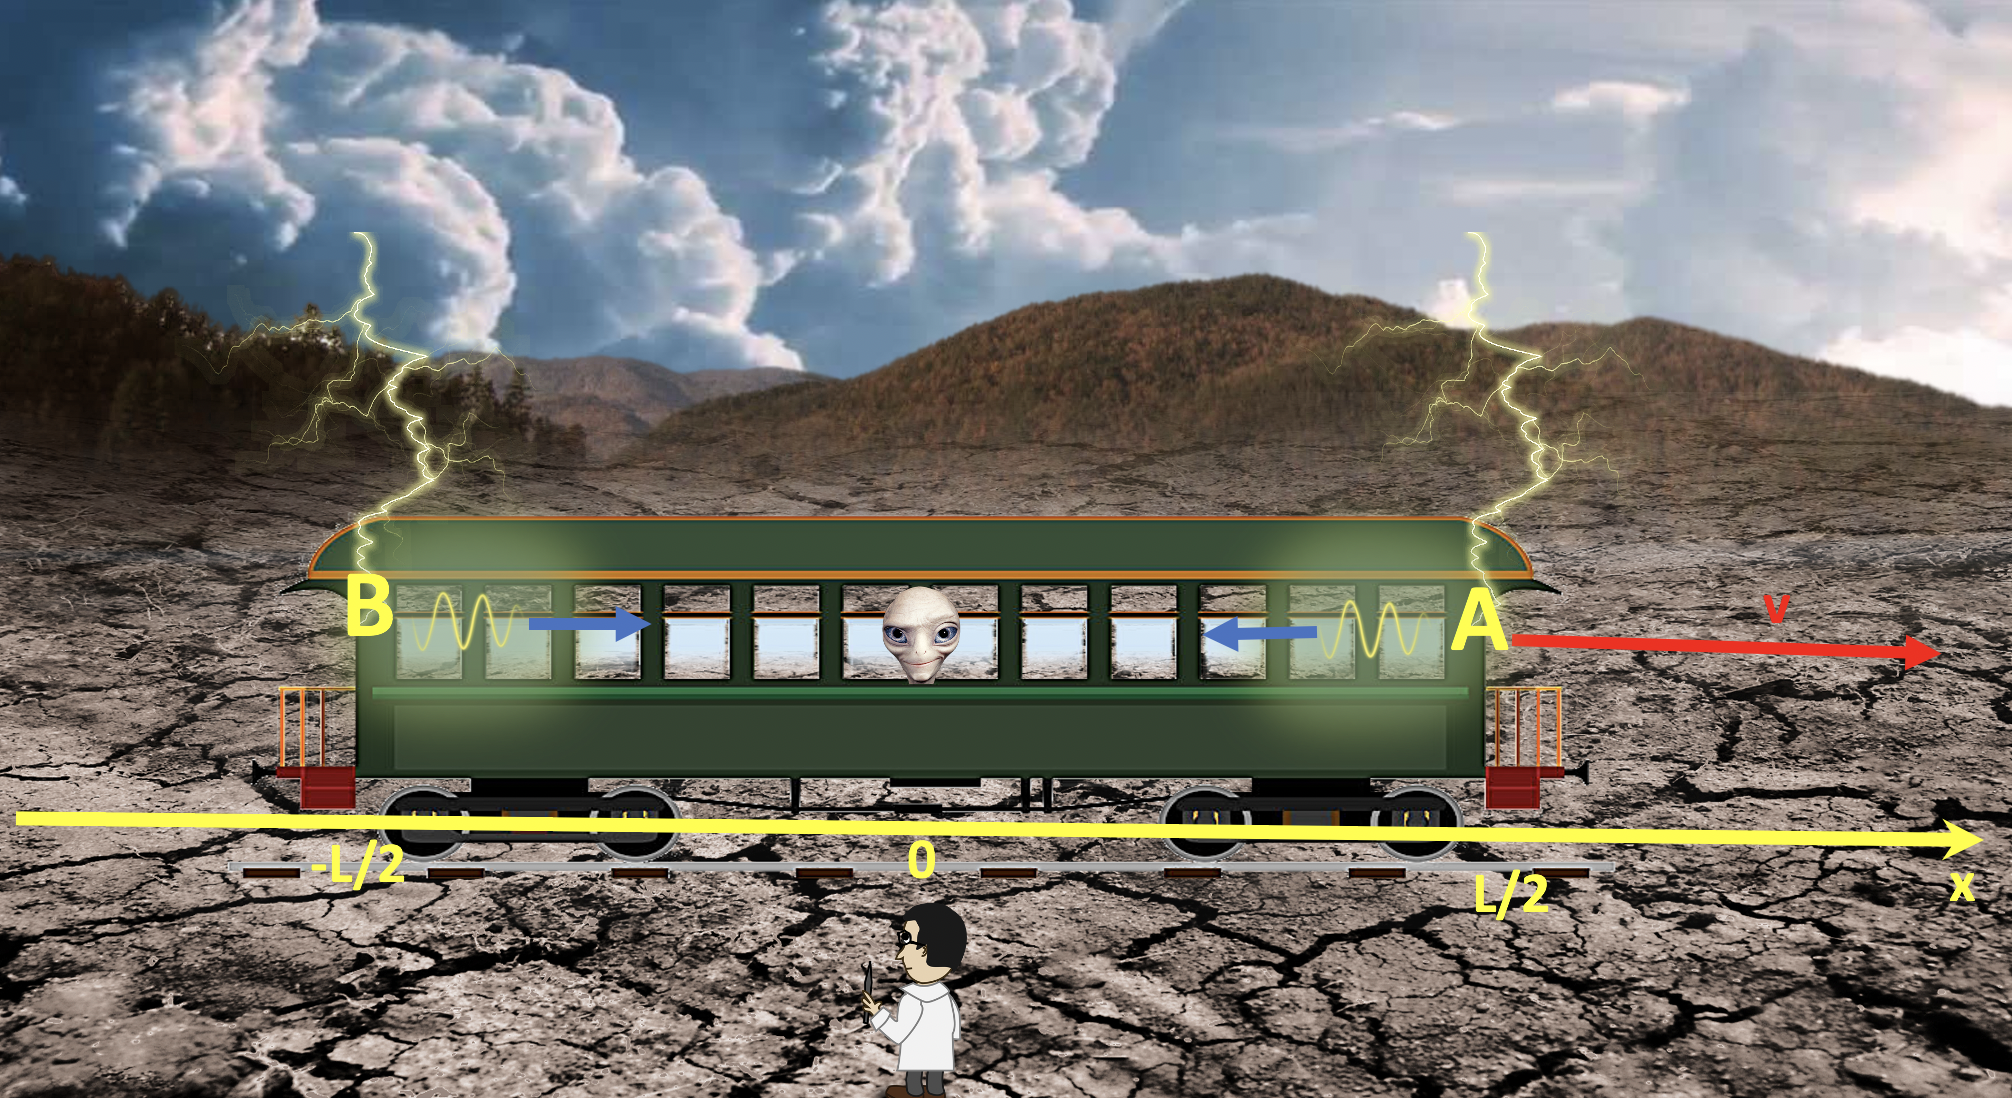
\includegraphics[scale=0.26]{media/tog1.png}}
Din oppgave nå er å finne tidspunktene når event C og event D skjer. Uttrykk svarene med togets lengde $L$ og lyshastigheten $c$.
}{SIDE 34/61/61}

\choiceframe{tog8}{tog7}{0}{
\centerline{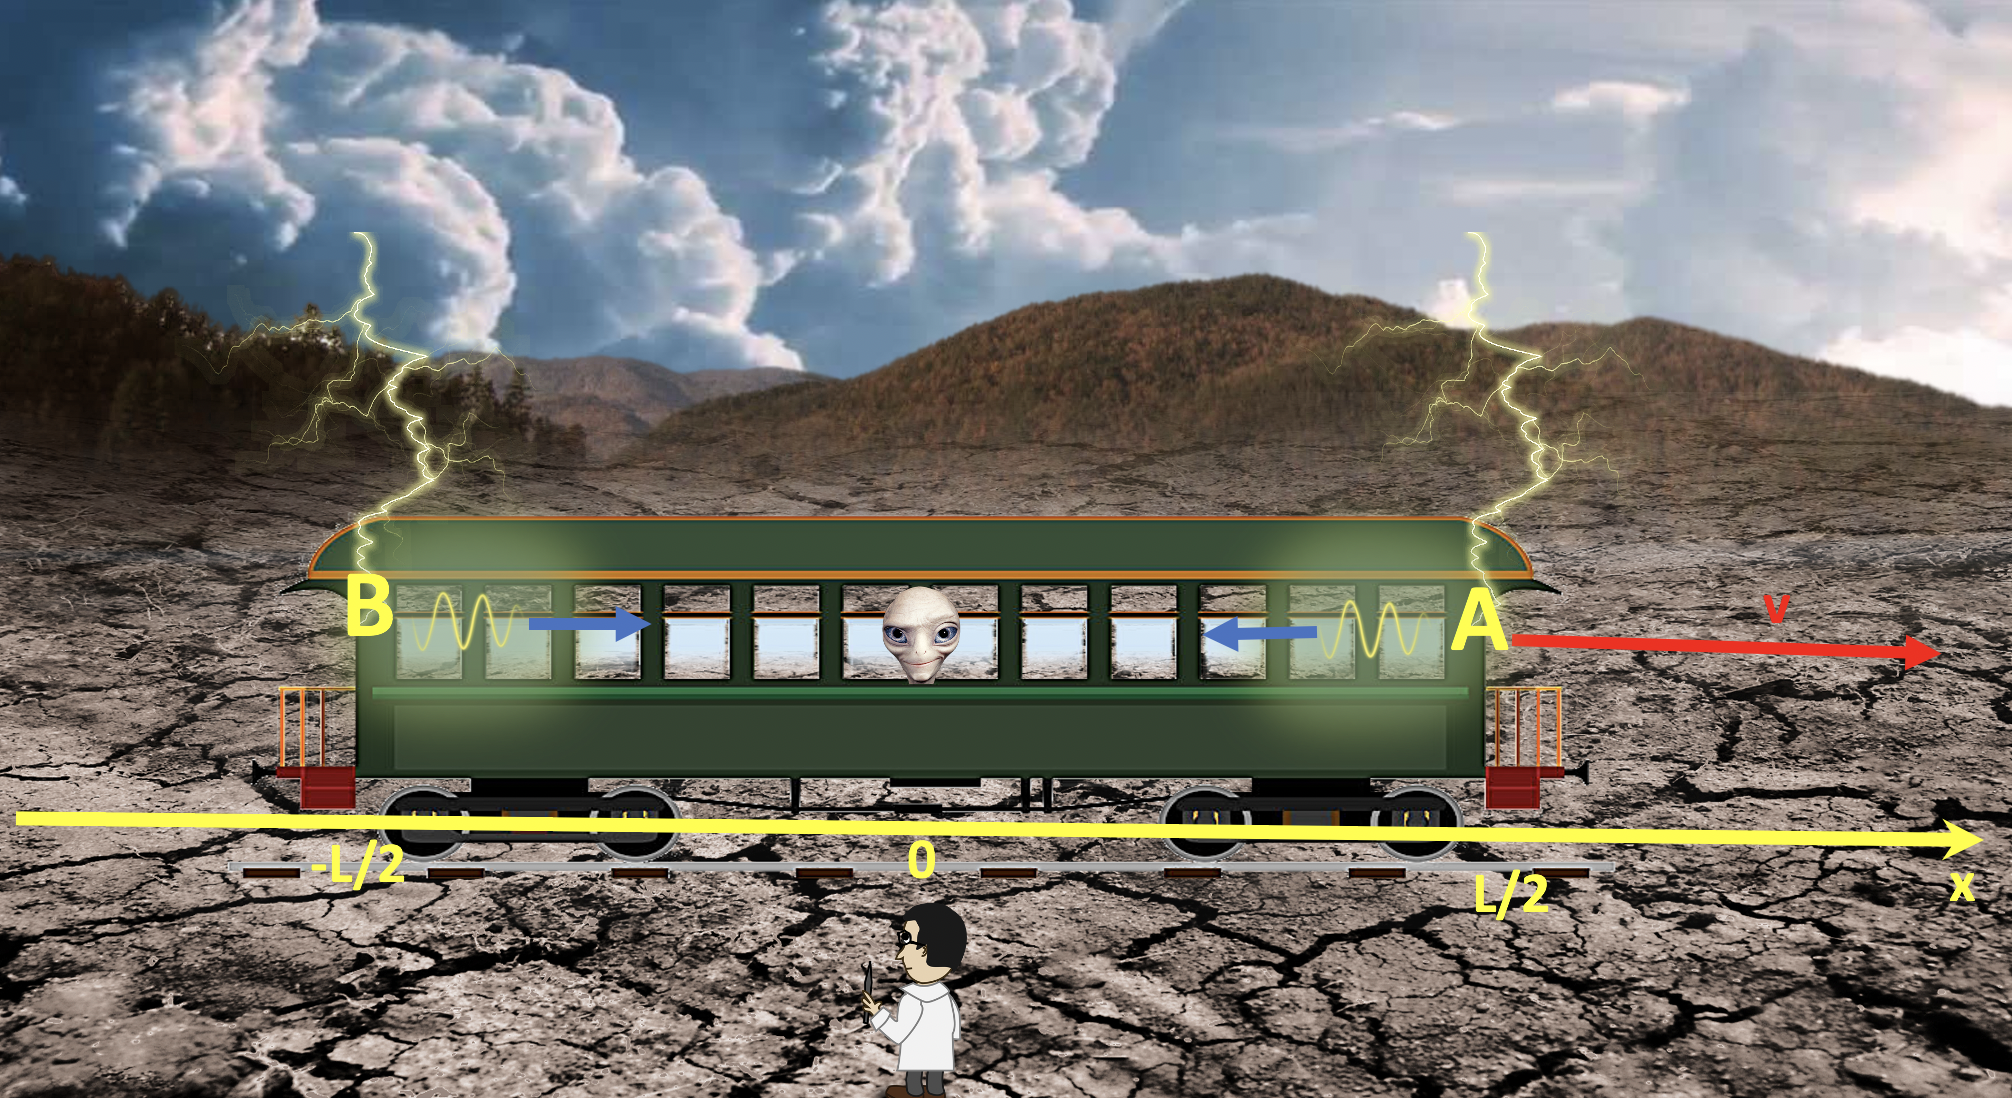
\includegraphics[scale=0.26]{media/tog1.png}}
Hva stemmer? \hyperlink{feil_tog8a}{\choicebutton{\small $t_c=L/2, \ \ t_D=L/2$}} \hyperlink{feil_tog8a}{\choicebutton{\small $t_c=L/(2v) - v/c, \ \ t_D=L/(2v) + v/c$}}\\
\hyperlink{feil_tog8a}{\choicebutton{\small $t_c=L\sqrt{1-(v/c)^2}/v,\ \ t_D=L/\sqrt{1-(v/c)^2}/v$}}\\
\hyperlink{riktig_tog8b}{\choicebutton{\small $t_c=L/2/(c+v), \ \ t_D=L/2/(c-v)$}}\hyperlink{feil_tog8a}{\choicebutton{\small $t_c=L/2/c, \ \ t_D=L/2/v$}}\\
\hyperlink{feil_tog8a}{\choicebutton{\small $t_c=(L-v)/2/c, \ \ t_D=(L+v)/2/c$}}
}{SIDE 35/61/61}

\colchoiceframe{feil_tog8a}{tog8}{0}{black}{\large
\textcolor{yellow}{Det ble galt! Gjorde du et skikkelig forsøk? Kanskje du kan skrive en funksjon for posisjonen til strålen fra A? Og så en funksjon for strålen fra B? Og når denne funksjonen er lik posisjonen til passasjer P (som du også trenger en funksjon for), da skjer event C og D? Hvis du kommer hit for andre gang, ta en titt på denne \href{https://www.uio.no/studier/emner/matnat/astro/AST2000/h20/undervisningsmateriell/interaktive-forelesningsnotater/2a/videoer/video2a_1.mp4}{videoen}}
}{SIDE 36/61/61}

\colfullframe{riktig_tog8b}{tog8}{pause}{-1}{yellow}{
\centerline{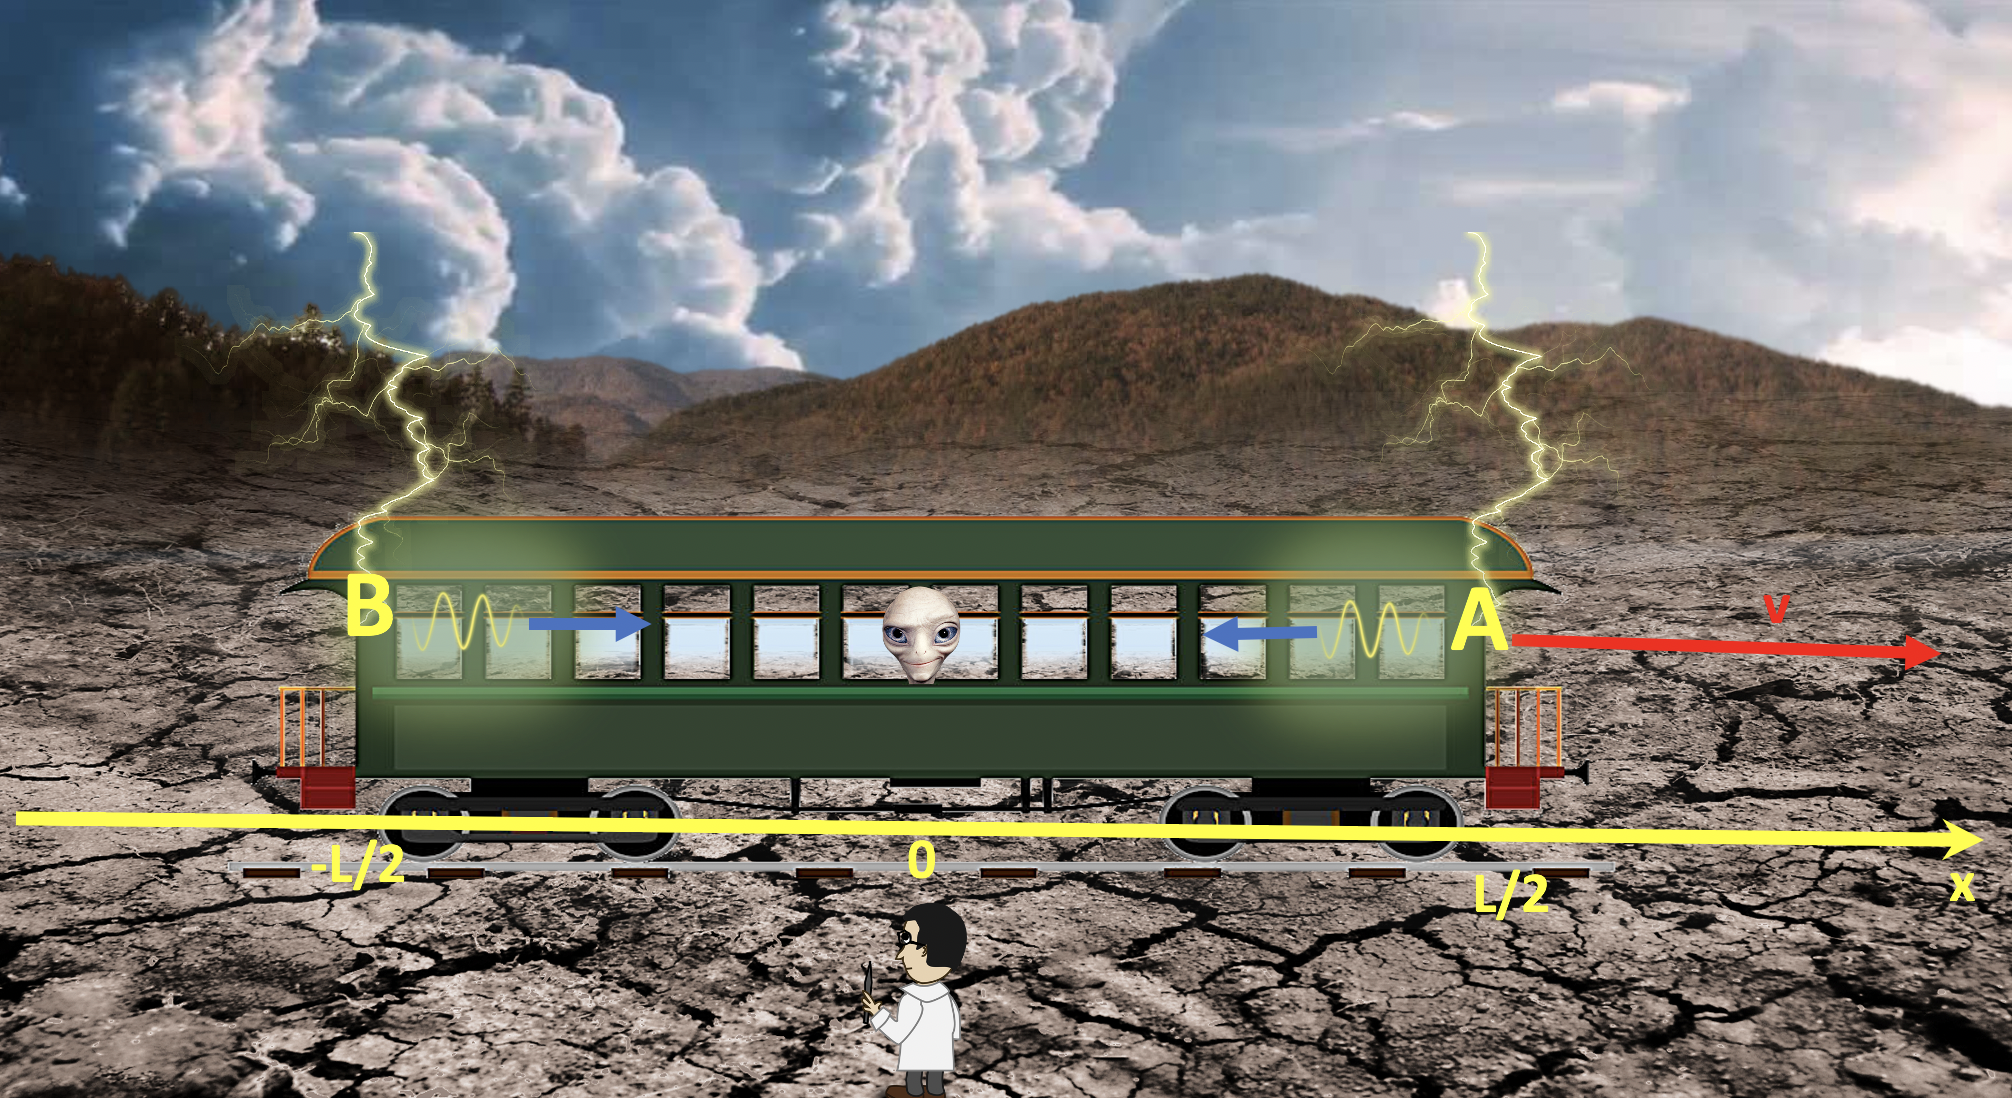
\includegraphics[scale=0.26]{media/tog1.png}}
Det er helt riktig! Hvis du enda er usikker,  ta en titt på denne \href{https://www.uio.no/studier/emner/matnat/astro/AST2000/h20/undervisningsmateriell/interaktive-forelesningsnotater/2a/videoer/video2a_1.mp4}{videoen}
}{SIDE 37/61/61}


{
\setbeamercolor{background canvas}{bg=cyan}
\begin{frame}
\label{pause}
\hyperlink{riktig_tog8b}{\pagebutton{\small Forrige side}}
{\huge
\centerline{Kaffe?}
\centerline{
\includegraphics[scale=4]{media/drink-coffee.png}}\\
Litt frisk luft nå! Ikke lov å bli inne. Vekk fra alle skjermer.
Ikke lov å fortsette før du har tatt minst 15 min. pause!
Og forbered hjernen på et sjokk: nå kommer selvmotsigelsen her...
}\\
\vspace*{0.5cm}
\hyperlink{tog9}{\pagebutton{Ok, jeg er klar...}}
\end{frame}
}


\fullframe{tog9}{riktig_tog8b}{tog10}{0}{
\centerline{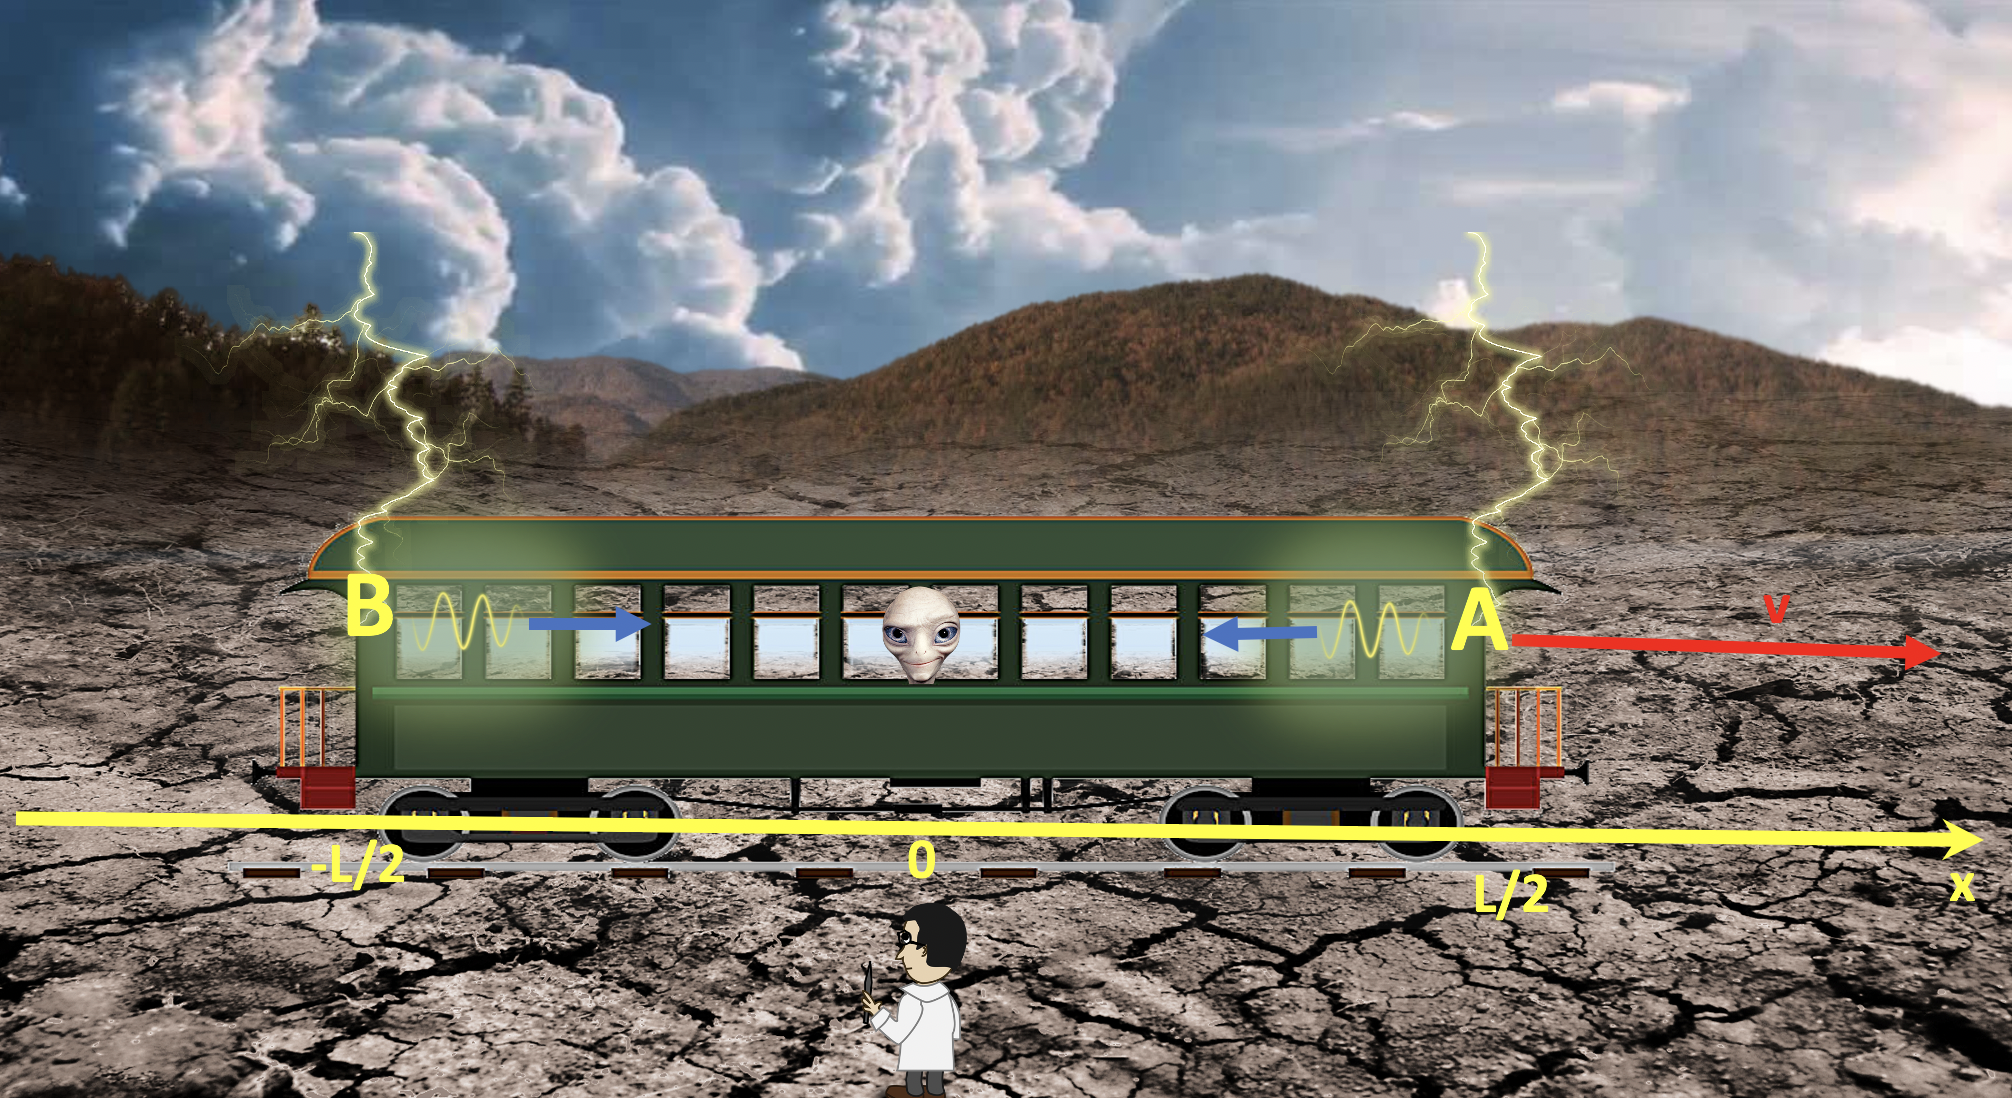
\includegraphics[scale=0.26]{media/tog1.png}}
Så vi fant at siden toget og passasjeren beveger seg mot lysstrålen fra A så vil passasjeren se lynnedslag A før lynnedslag B, selv om begge skjedde samtidig, ok? Og tidspunktet for event C og D som er passasjerens observasjoner av henholdsvis lynnedslag A og B er
\[
t_C=\frac{L/2}{c+v},\ \ t_D=\frac{L/2}{c-v}
\]
}{SIDE 38/61/61}


\fullframe{tog10}{tog9}{tog11}{0}{
\centerline{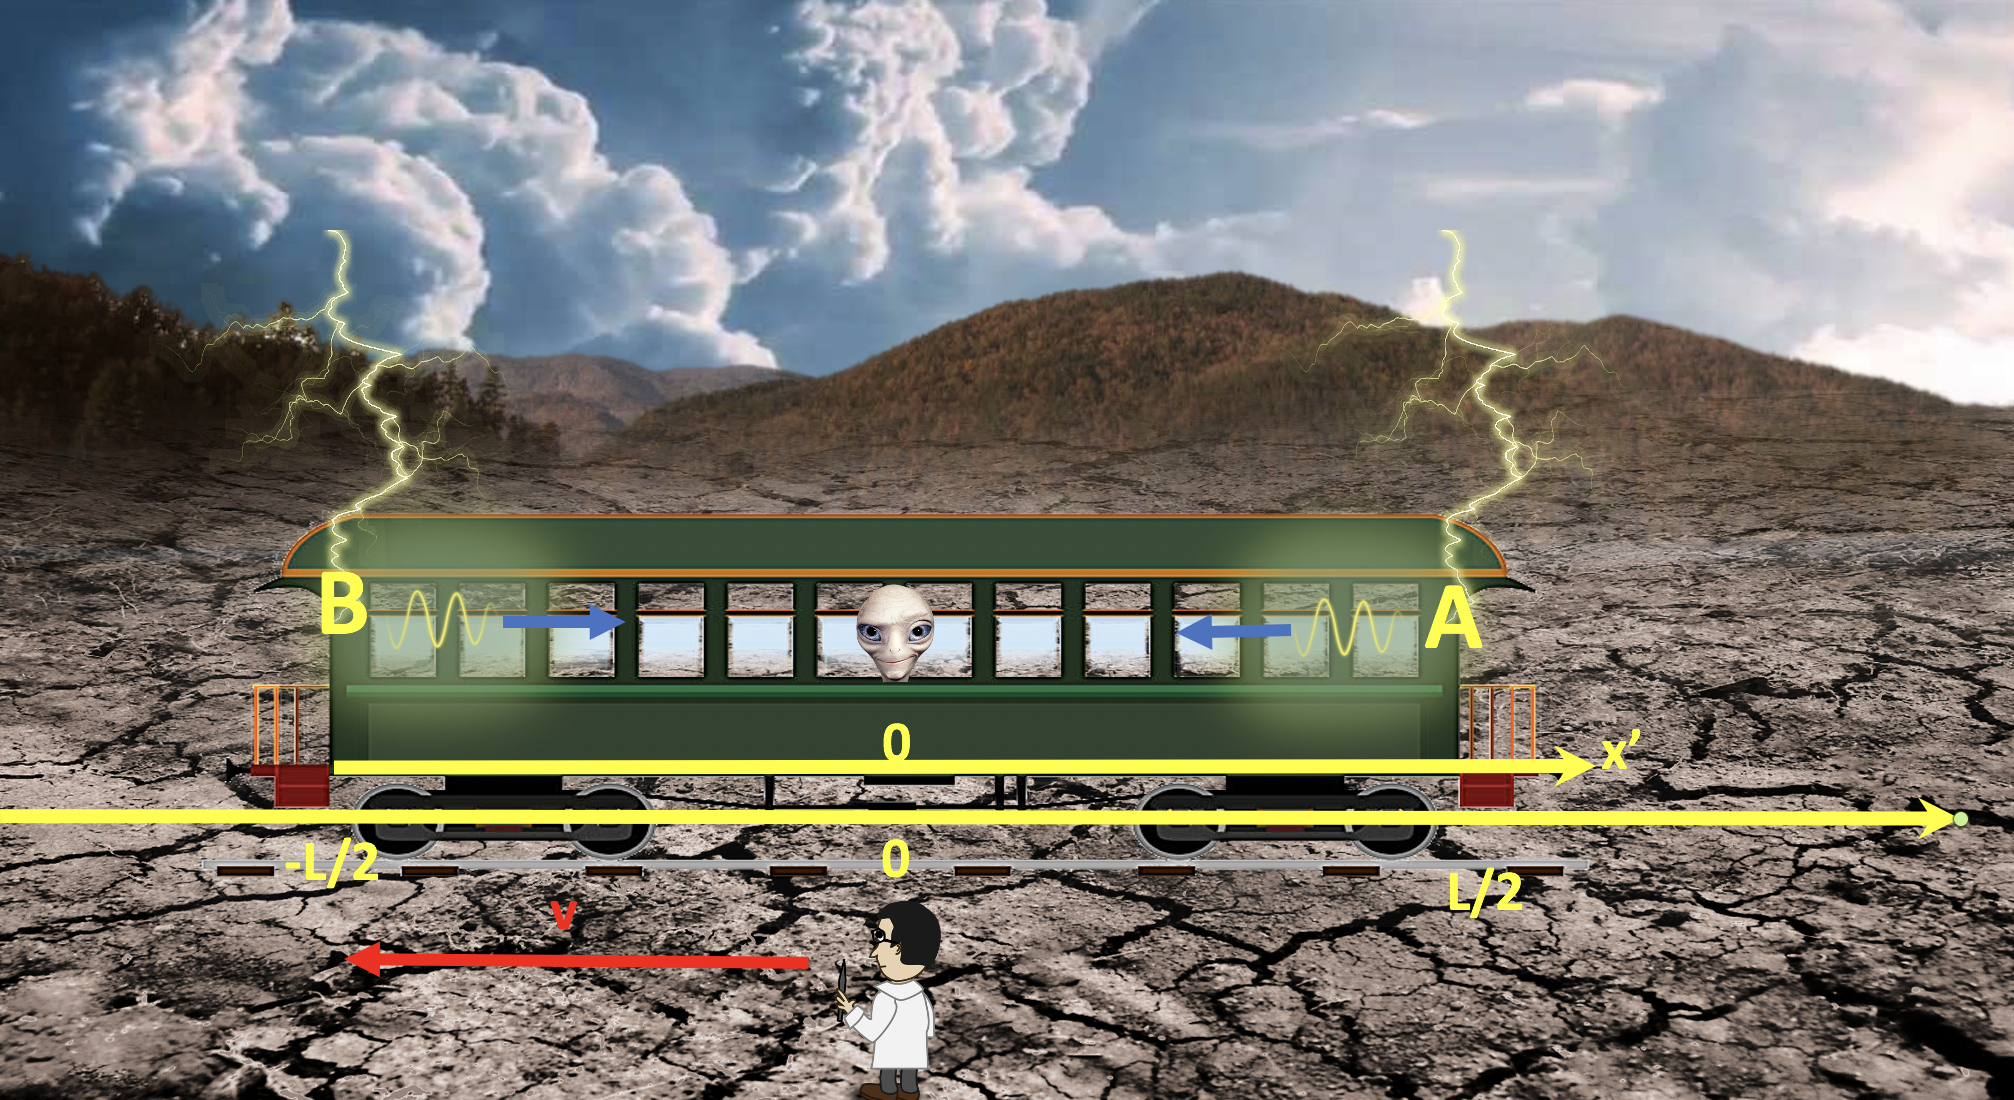
\includegraphics[scale=0.26]{media/tog4.png}}
La oss regne på situasjonen {\bf en gang til}. Men nå flytter vi oss til passasjer P sitt referansesystem. I dette referansesystemet står toget stille mens bakken, professor O og x-aksen (som står fast på bakken) beveger seg bakover. Vi har innført en egen merket $x'$-akse som står fast på toget og måler alle posisjoner i forhold til toget. Passasjer P står på origo på denne aksen.
}{SIDE 39/61/61}

\fullframe{tog11}{tog10}{tog12}{0}{
\centerline{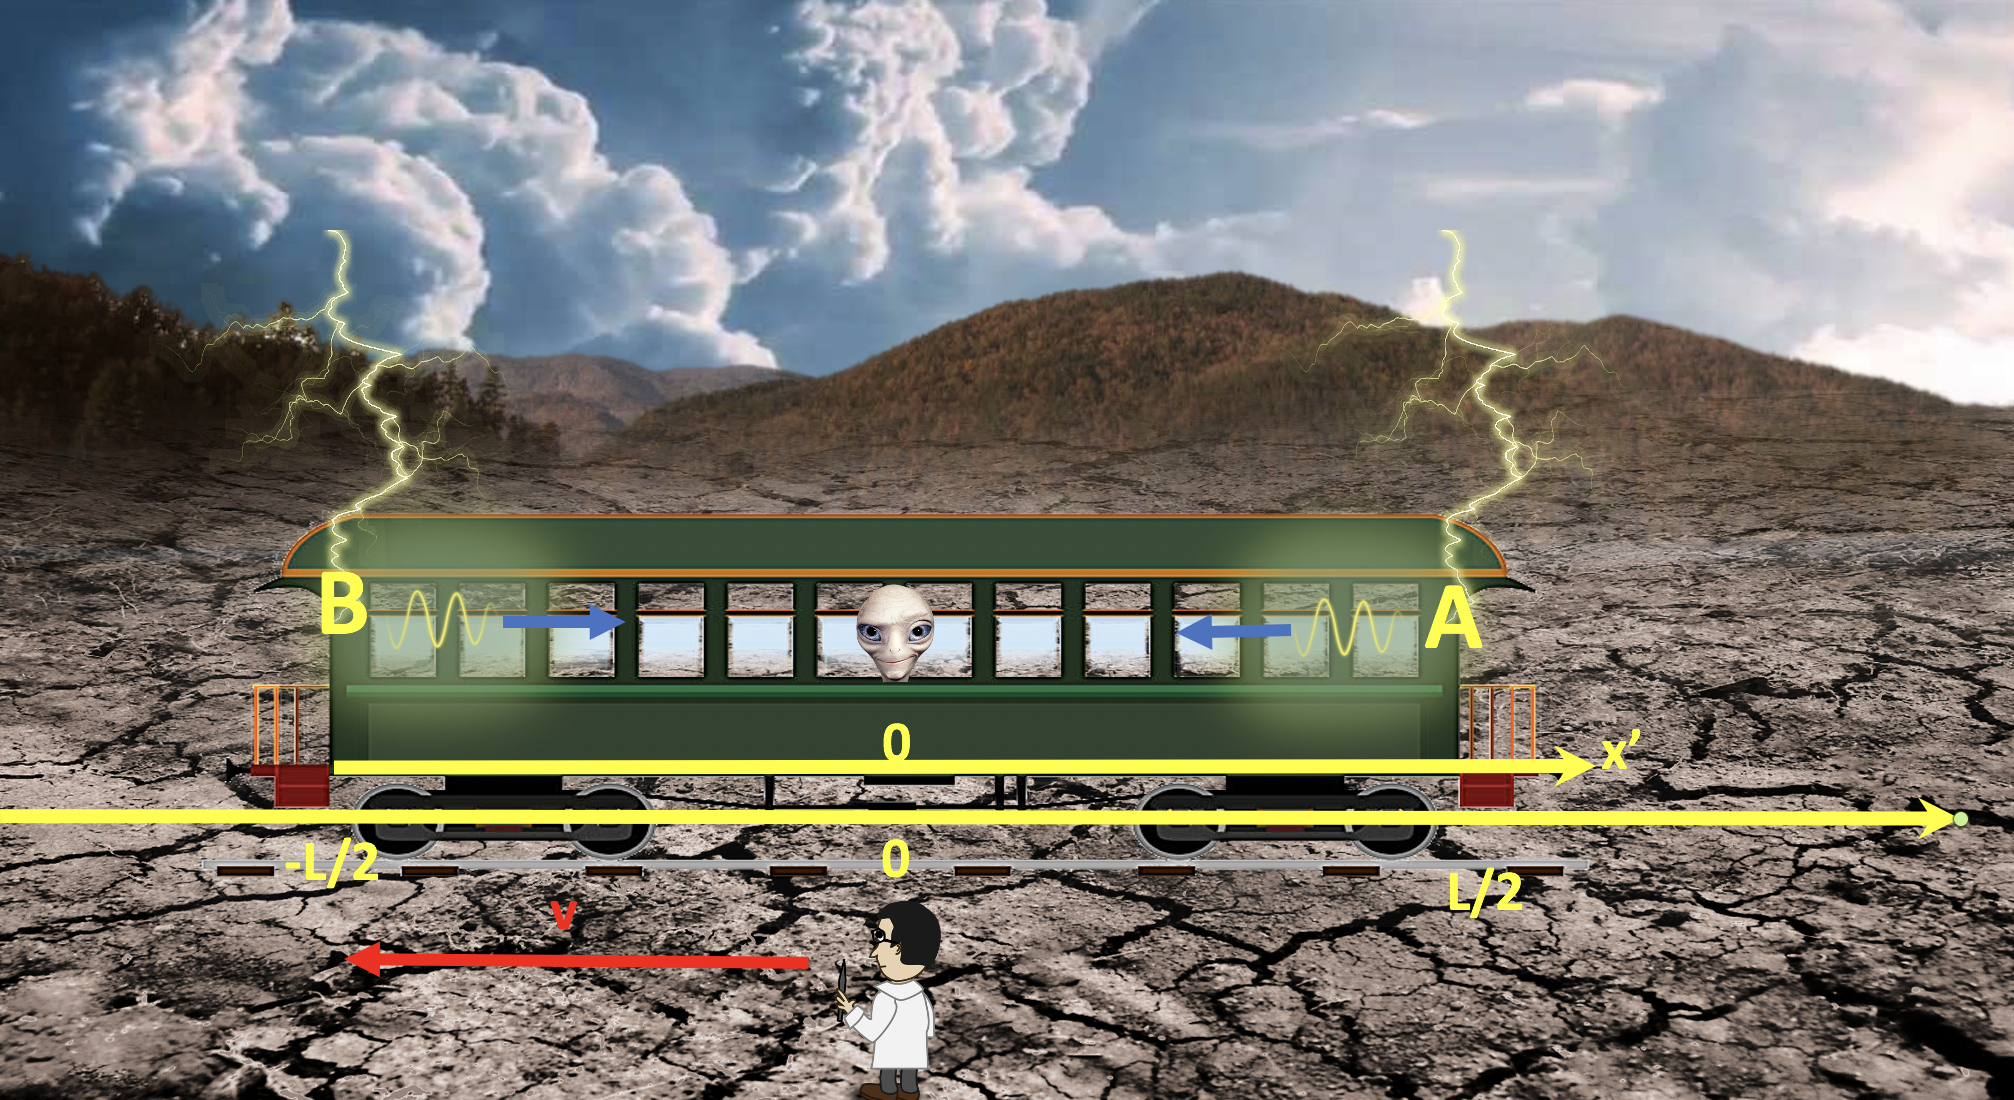
\includegraphics[scale=0.26]{media/tog4.png}}
Hvordan blir det nå? Vi har jo nøyaktig den samme situasjonen, vi bare regner fra et annet referansesystem. Da bør vi få samme svar. Gjør vi det? Toget står altså stille, bakken beveger seg med hastighet $v$ bakover, lysstrålene fra lynnedslagene beveger seg med lysets hastighet. Hva skjer?
\hyperlink{riktig_tog11b}{\choicebutton{P ser begge samtidig}}\hyperlink{feil_tog11a}{\choicebutton{P ser A før B}}\hyperlink{feil_tog11a}{\choicebutton{P ser B før A}}
}{SIDE 40/61/61}


\colchoiceframe{feil_tog11a}{tog11}{0}{black}{\large
\textcolor{yellow}{Neeeei, ikke helt! Beveger passasjer P seg nå i forhold til lysstrålene? Går en av lysstrålene fortere enn den andre eller går de like fort? (hint: dette er lys!) Hvor lang avstand har hver av lysstrålene å tilbakelegge frem til passasjer P?}
}{SIDE 41/61/61}

\colfullframetxt{riktig_tog11b}{tog11}{tog12}{-1}{yellow}{Joa...}{
\centerline{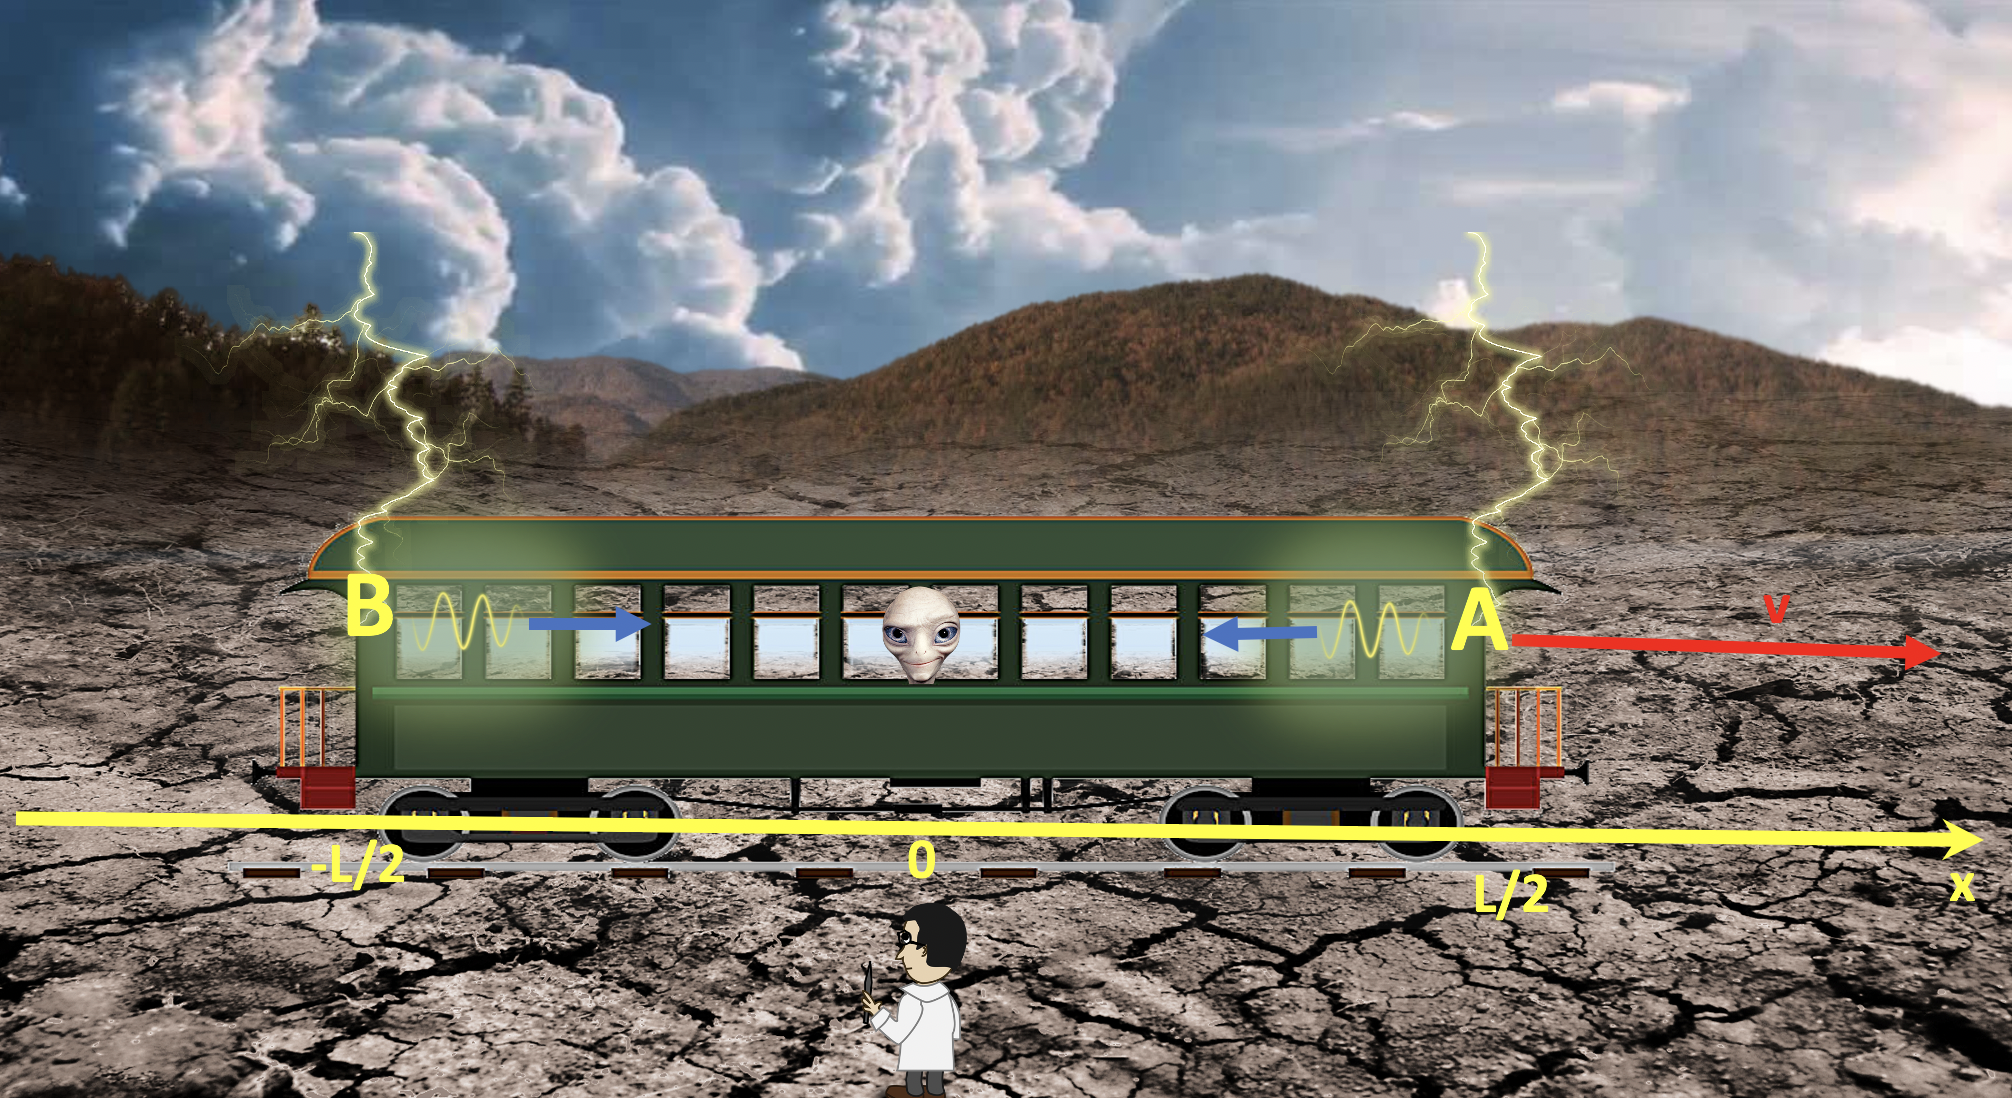
\includegraphics[scale=0.26]{media/tog1.png}}
Det stemmer. Må det ikke bli slik da: toget (og dermed passasjer P) står i ro. Begge lysstrålene har en avstand $L/2$ å tilbakelegge med samme hastighet $c$. Vil de ikke treffe passasjeren samtidig? Vil ikke passasjeren se begge lynnedslag samtidig?
}{SIDE 42/61/61}

\choiceframe{tog12}{riktig_tog11b}{0}{
\centerline{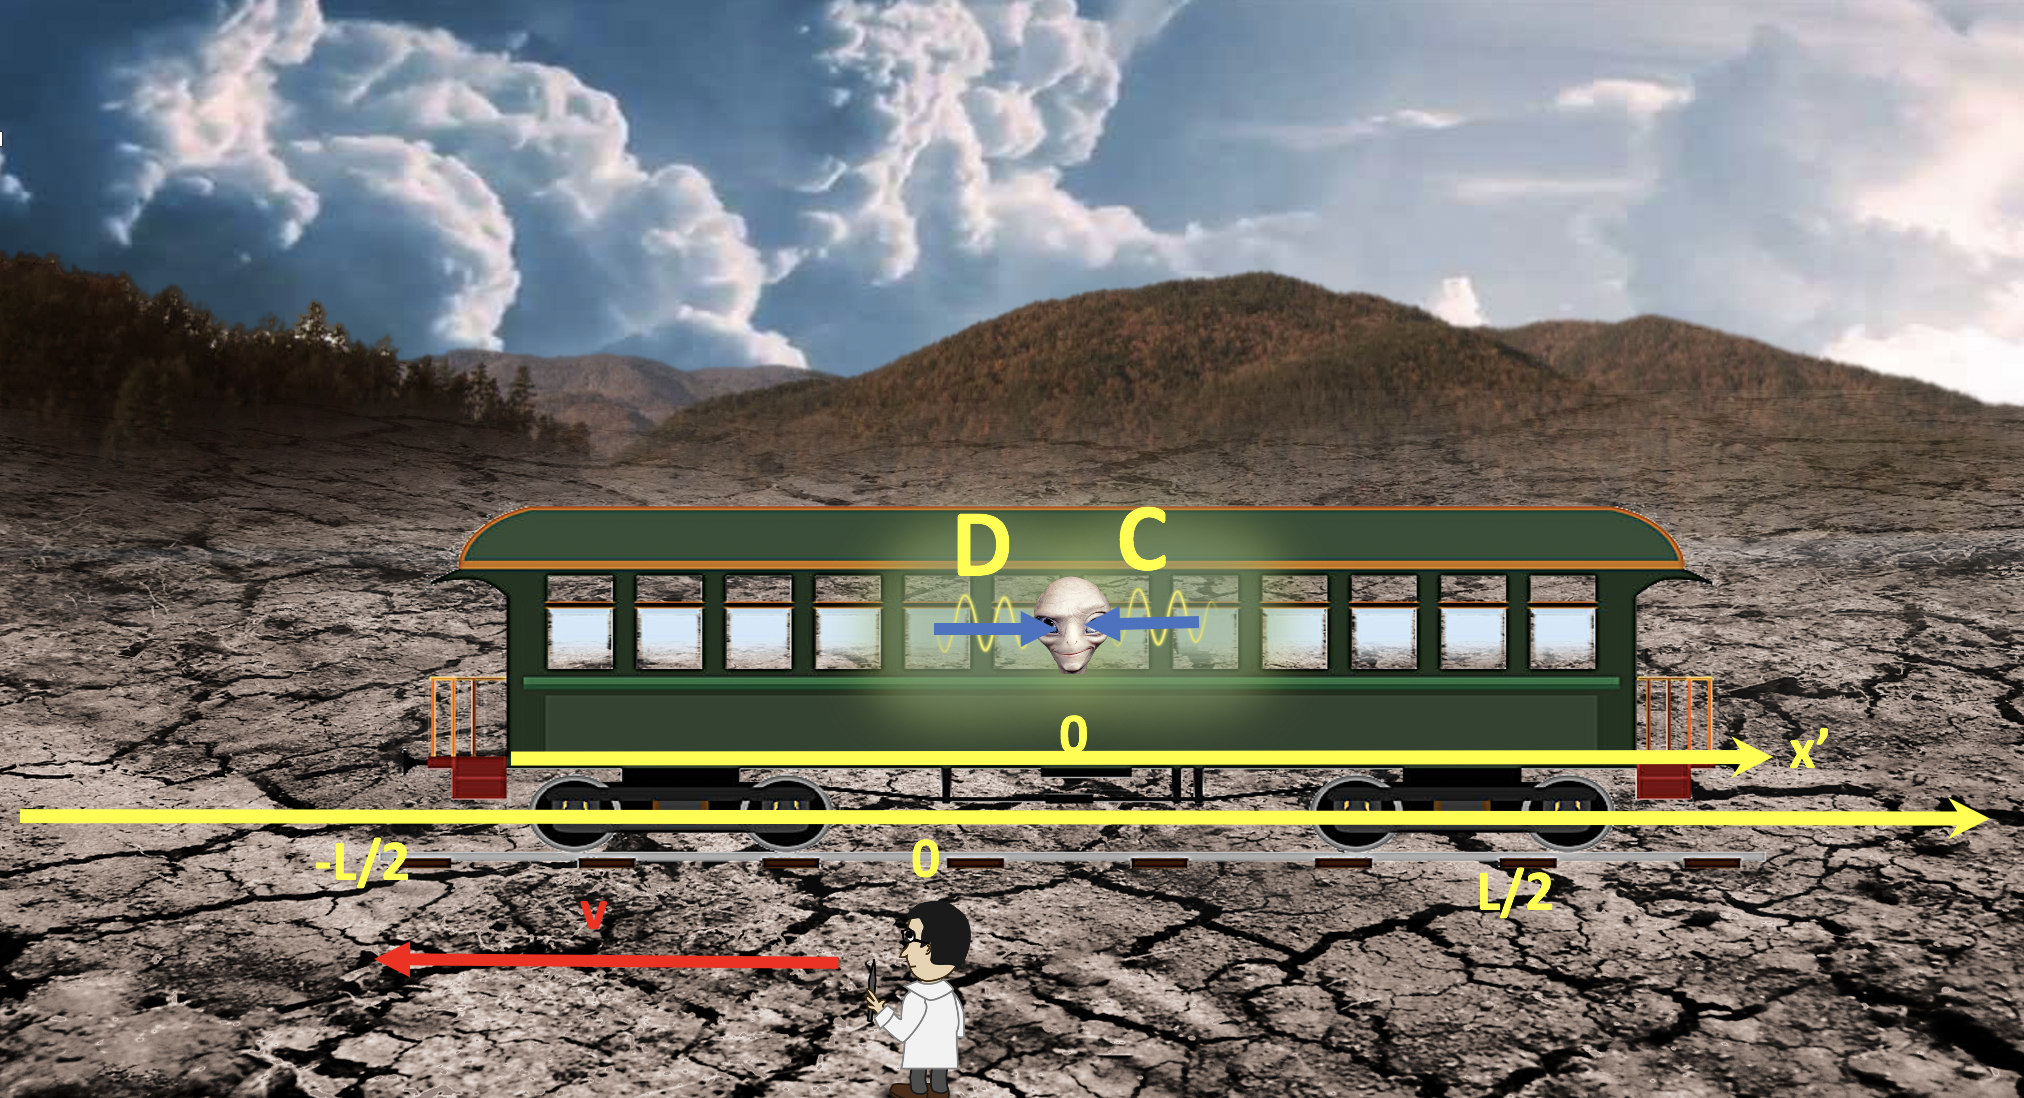
\includegraphics[scale=0.26]{media/tog5.png}}
Når skjer event C og D? Hvor lang tid tar det for strålene å nå passasjer P?\\
\hyperlink{feil_tog12a}{\choicebutton{\small $t_c=t_D=L\sqrt{1-(v/c)^2}/v$}}\\
\hyperlink{feil_tog12a}{\choicebutton{\small $t_c=t_D=L/2/(c+v)$}}\hyperlink{riktig_tog12b}{\choicebutton{\small $t_c=t_D=L/2/c$}}\\
\hyperlink{feil_tog12a}{\choicebutton{\small $t_c=t_D=(L-v)/2/c$}}
}{SIDE 43/61/61}


\colchoiceframe{feil_tog12a}{tog12}{0}{black}{\large
\textcolor{yellow}{Det ble galt! Gjorde du et skikkelig forsøk? Hvor lang avstand skal lysstrålene tilbakelegge? Med hvilken hastighet? Hvis du kommer hit for andre gang, ta en titt på denne \href{https://www.uio.no/studier/emner/matnat/astro/AST2000/h20/undervisningsmateriell/interaktive-forelesningsnotater/2a/videoer/video2a_2.mp4}{videoen}}
}{SIDE 44/61/61}

\colfullframe{riktig_tog12b}{tog12}{tog13}{-1}{yellow}{
\centerline{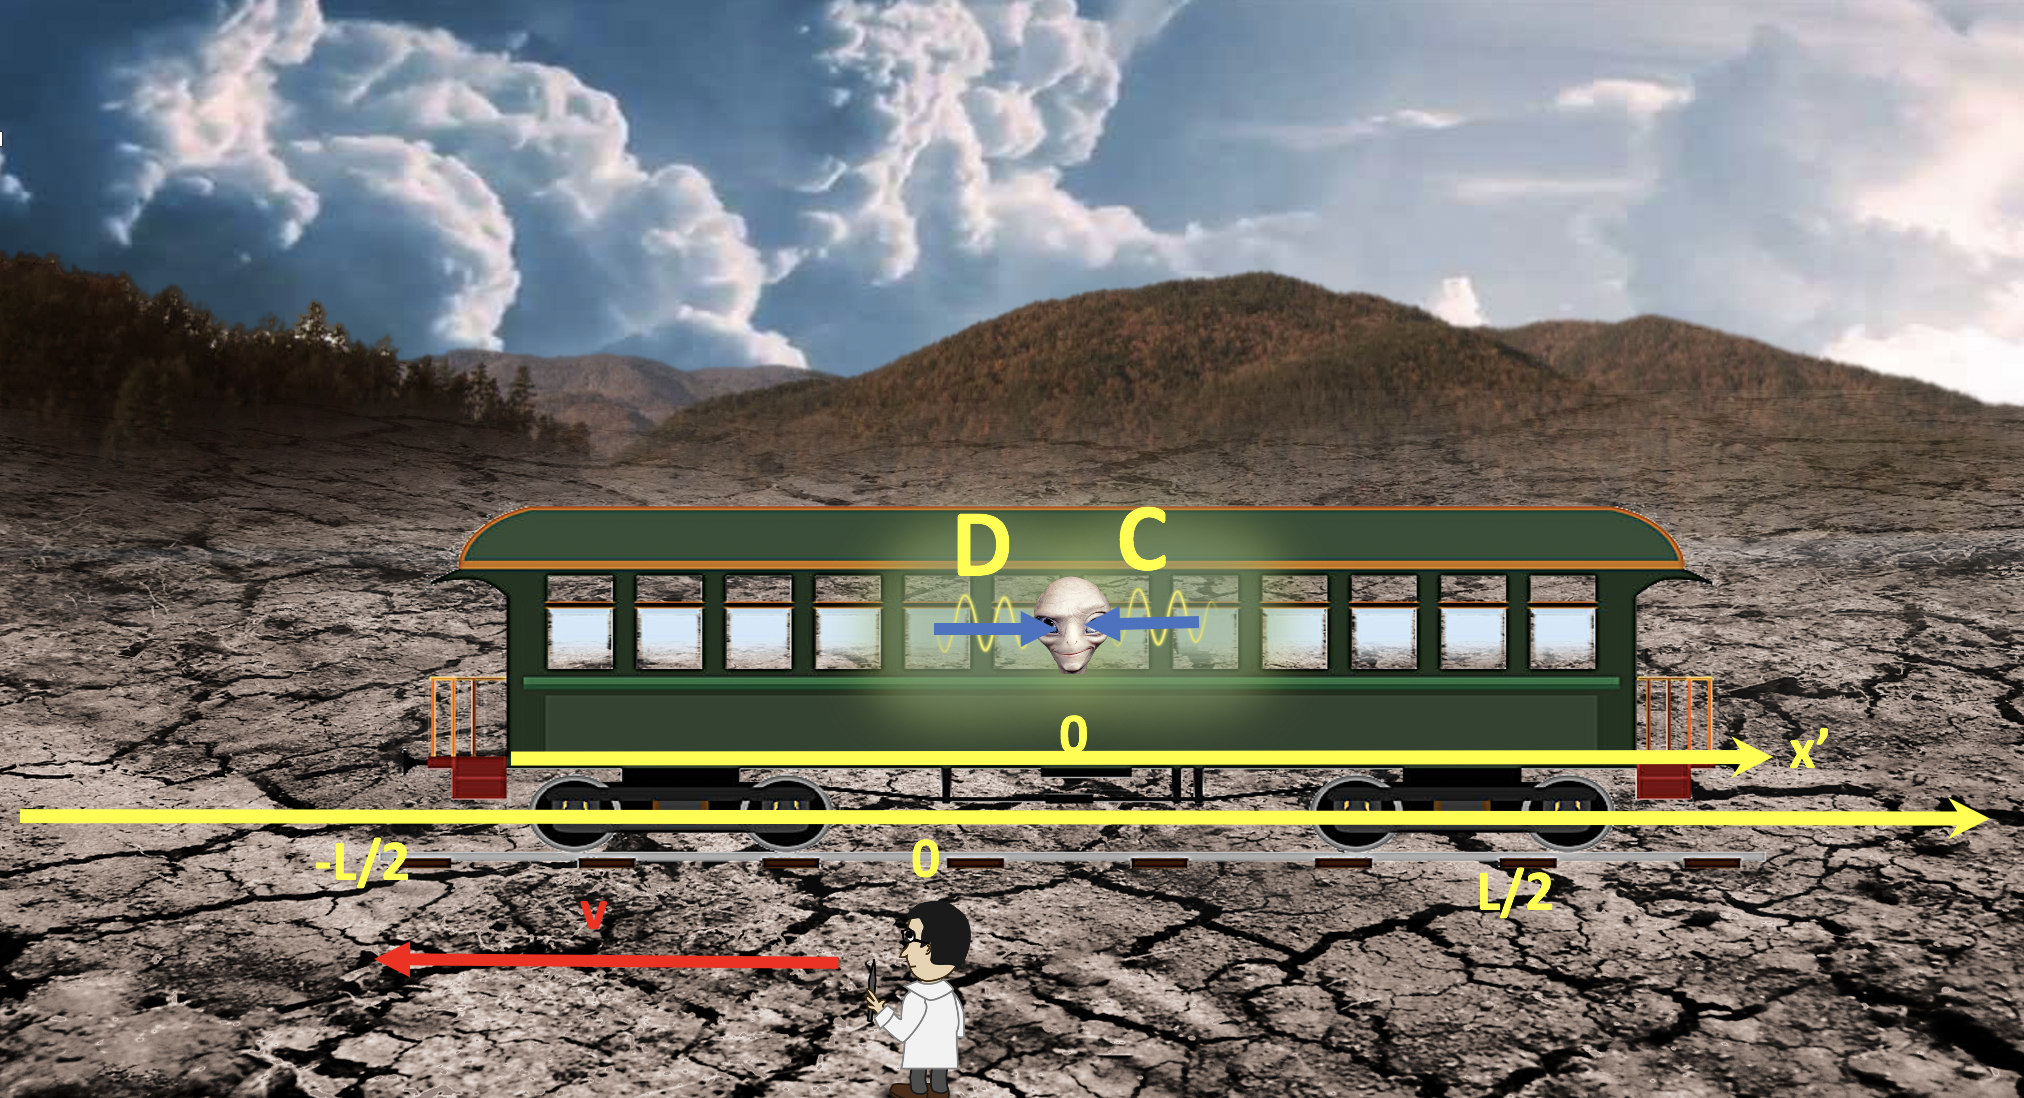
\includegraphics[scale=0.26]{media/tog5.png}}
Det er helt riktig! Hvis du enda er usikker, ta en titt på denne \href{https://www.uio.no/studier/emner/matnat/astro/AST2000/h20/undervisningsmateriell/interaktive-forelesningsnotater/2a/videoer/video2a_2.mp4}{videoen}
}{SIDE 45/61/61}

\fullframe{tog13}{riktig_tog12b}{tog14}{0}{\Huge
Men hva iallverden er rett da??? Ser passasjer P lysglimtene {\bf samtidig} eller {\bf A før B?}. Har vi gjort noe galt i noen av regningene?
}{SIDE 46/61/61}

\fullframe{tog14}{tog13}{tog15}{0}{\Huge
La oss spørre passasjer P selv hva hun så da! Og også professor P...
}{SIDE 47/61/61}

\colfullframe{tog15}{tog14}{tog16}{0}{silver}{
\centerline{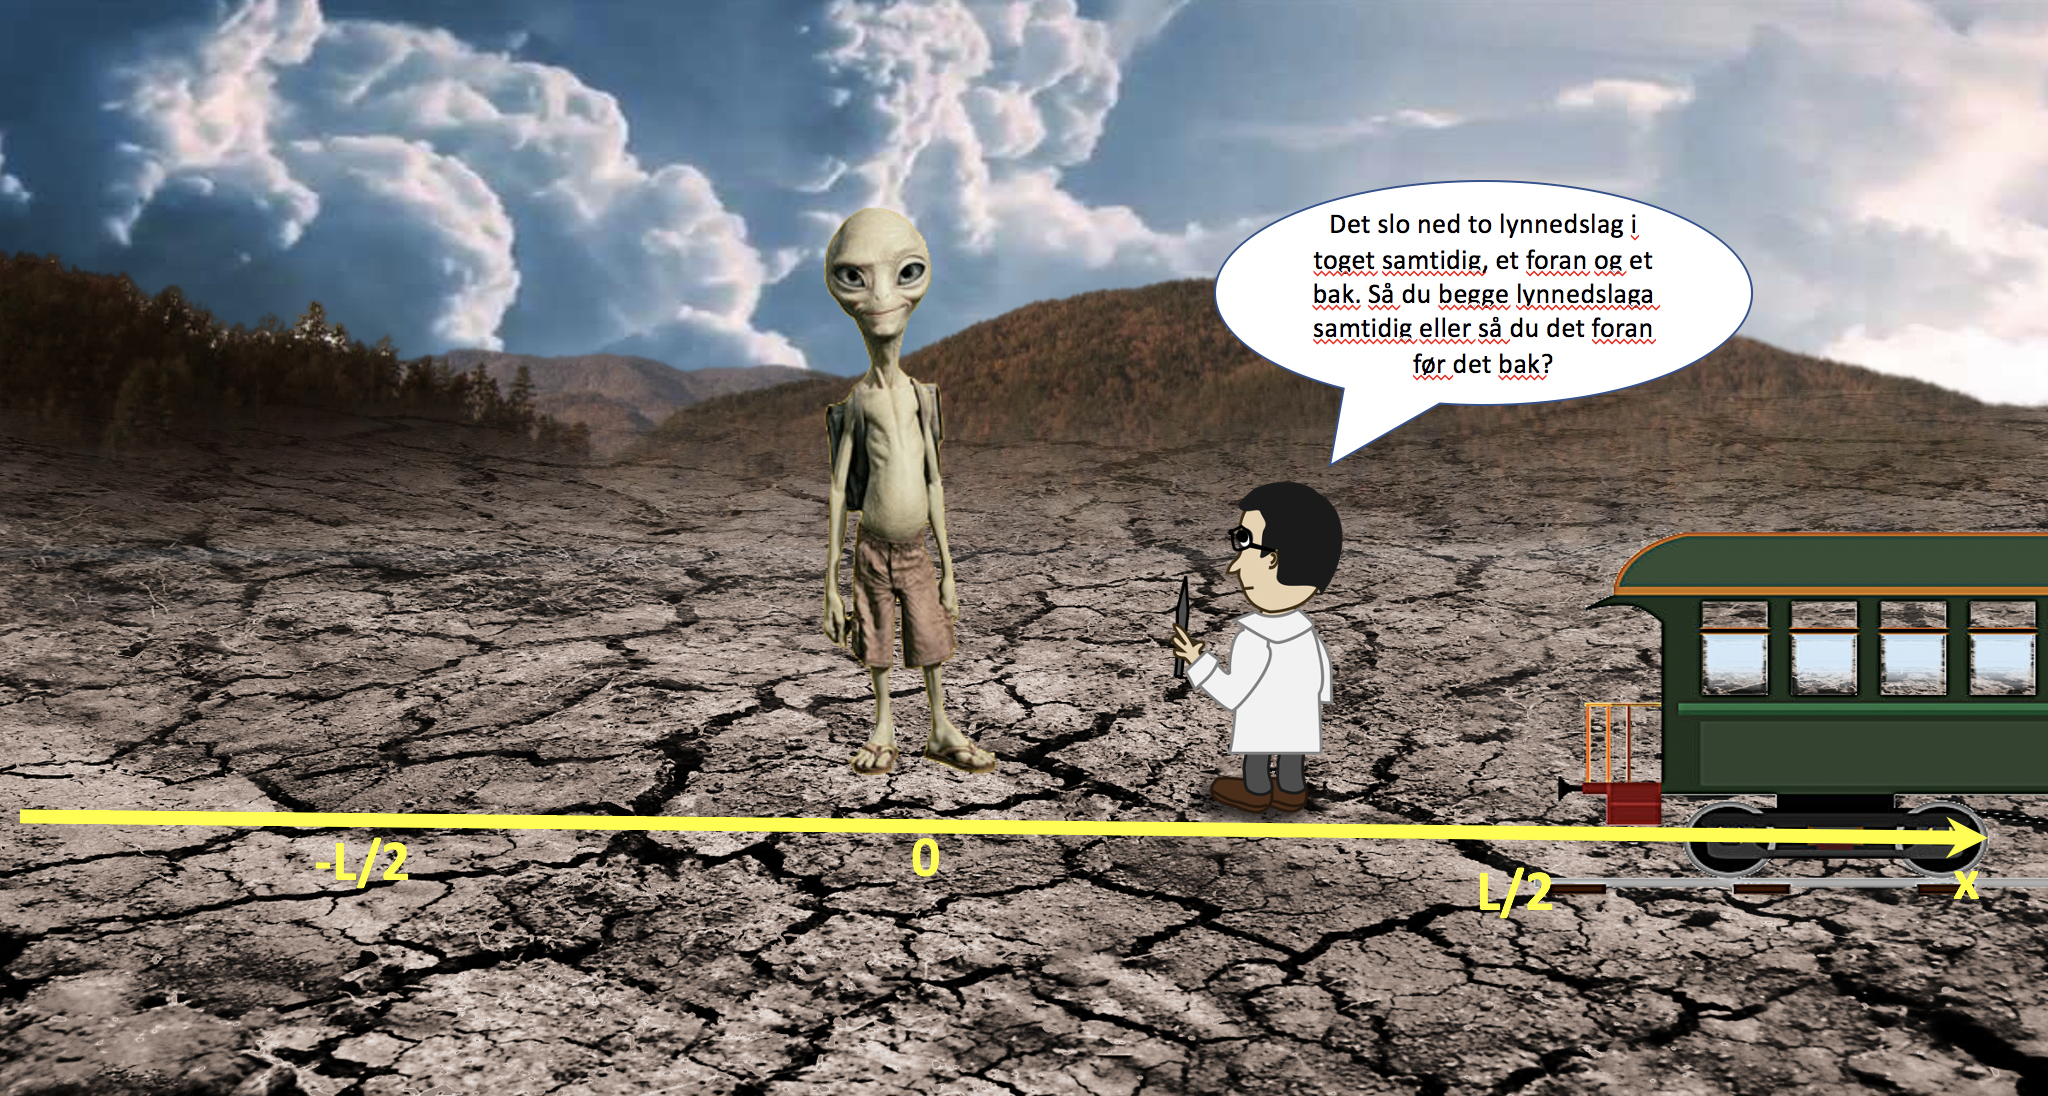
\includegraphics[scale=0.4]{media/samtale1.png}}
}{SIDE 48/61/61}

\colfullframe{tog16}{tog15}{tog17}{0}{silver}{
\centerline{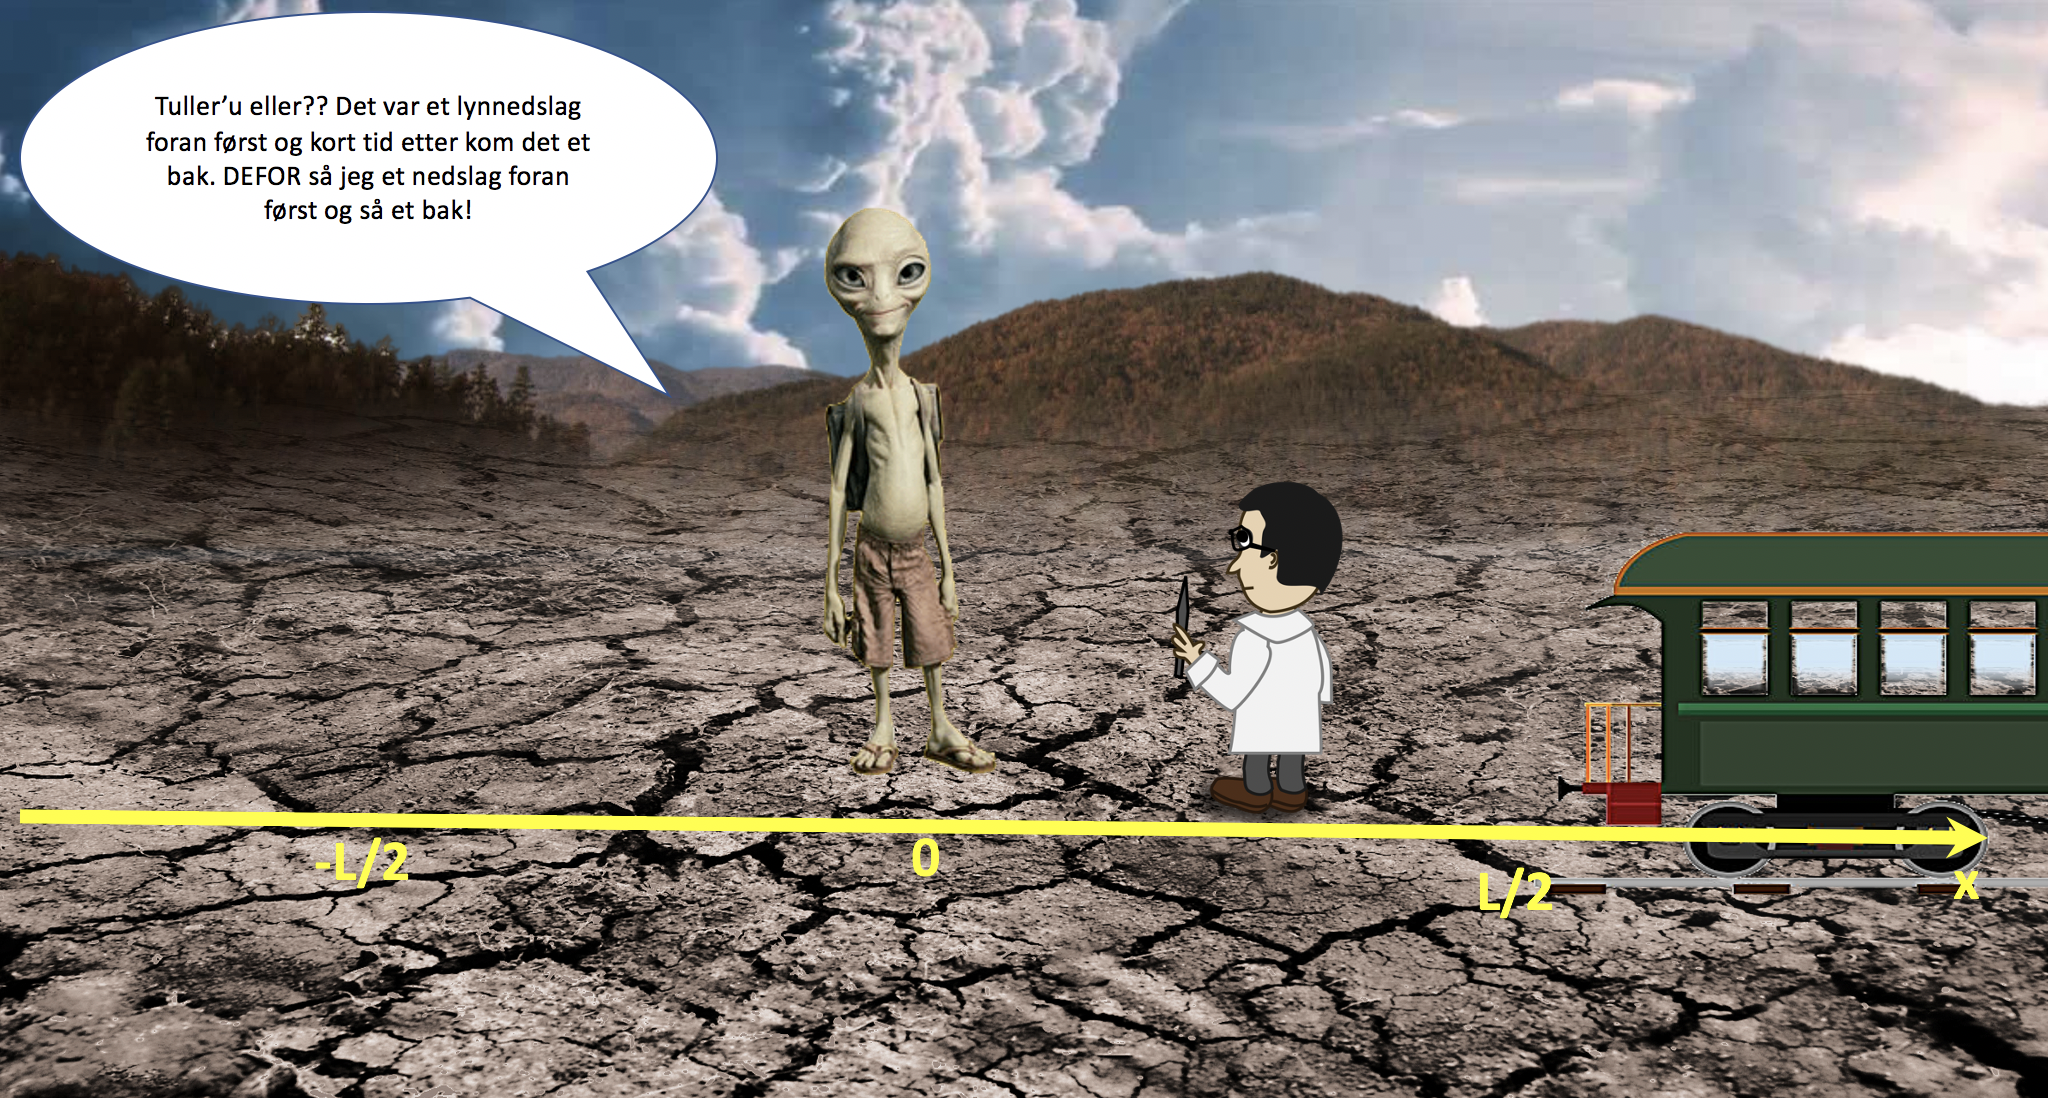
\includegraphics[scale=0.4]{media/samtale2.png}}
}{SIDE 49/61/61}

\colfullframe{tog17}{tog16}{tog18}{0}{silver}{
\centerline{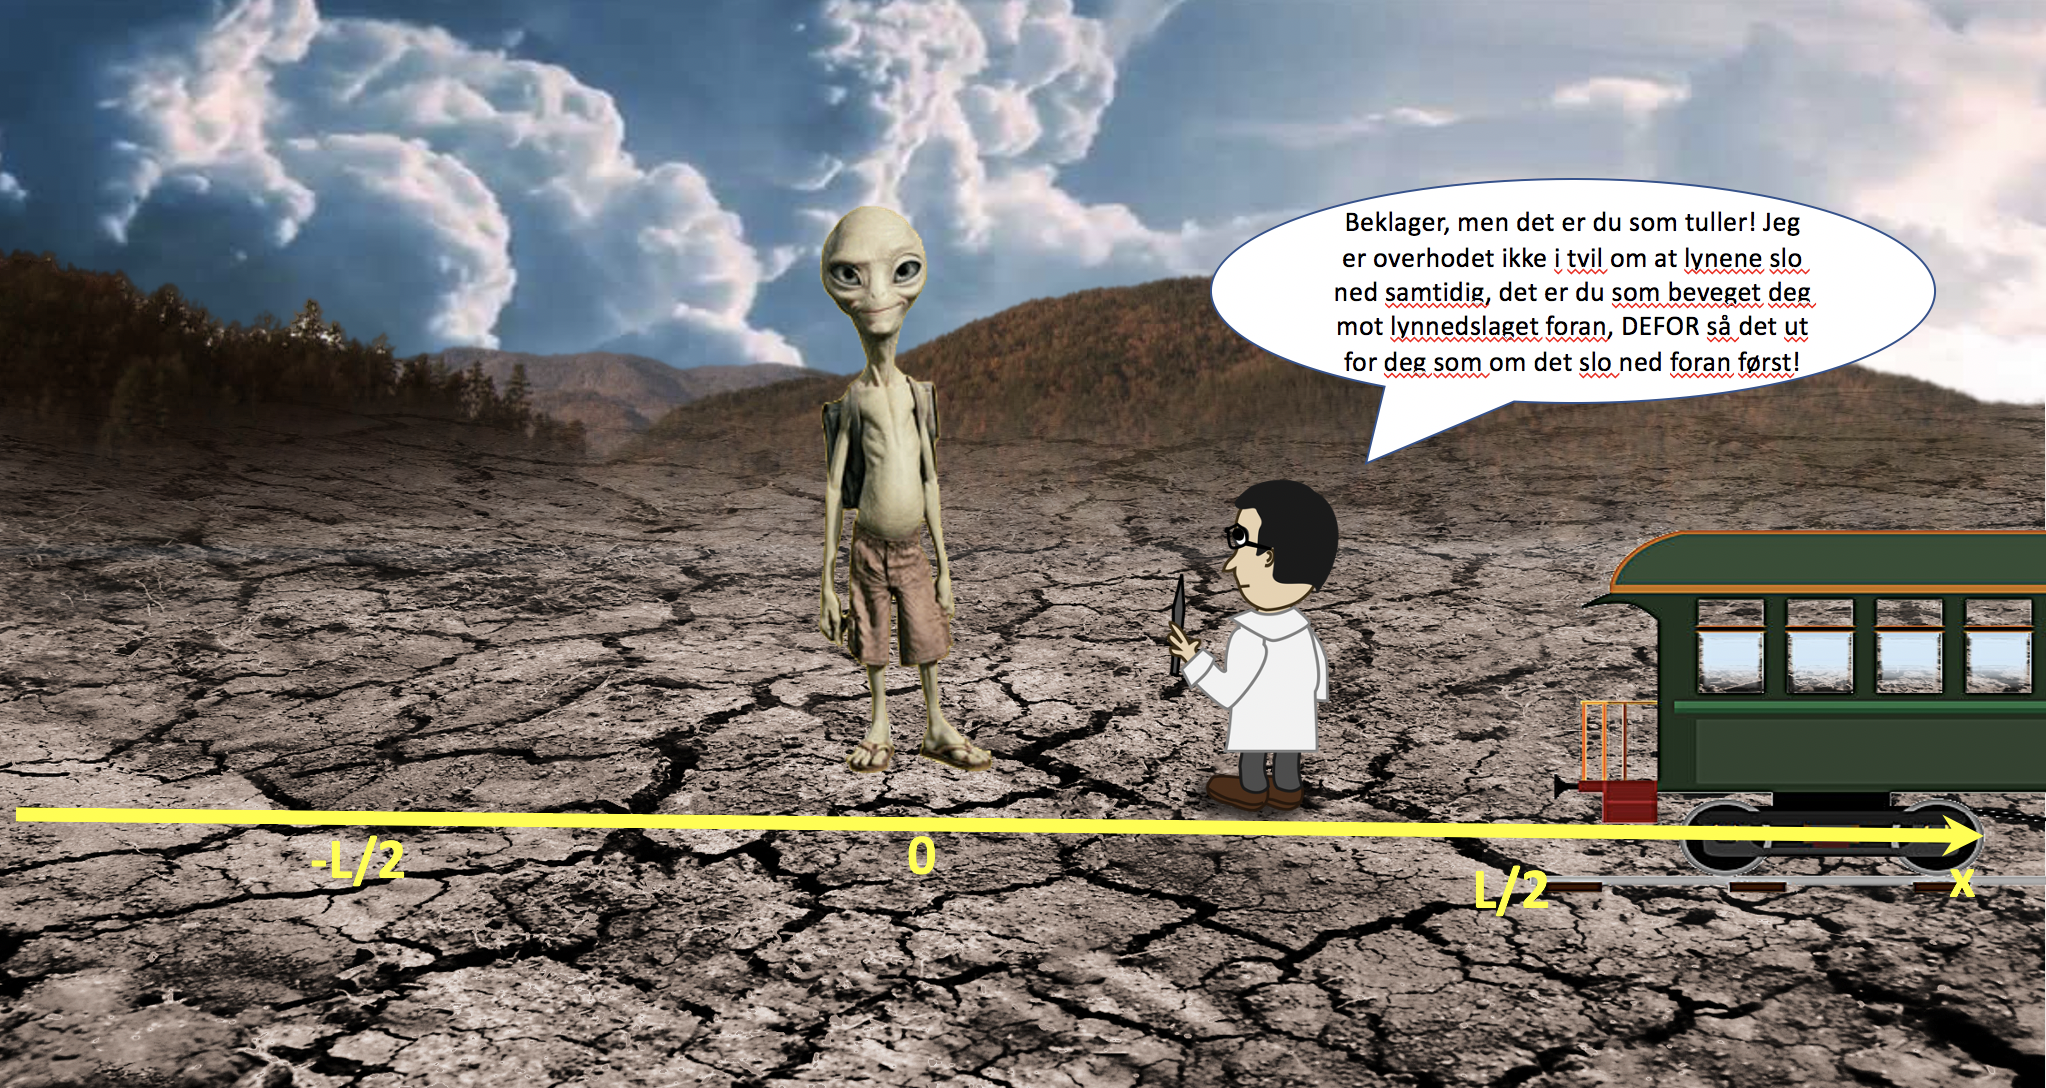
\includegraphics[scale=0.4]{media/samtale3.png}}
}{SIDE 50/61/61}

\colfullframe{tog18}{tog17}{tog19}{0}{silver}{
\centerline{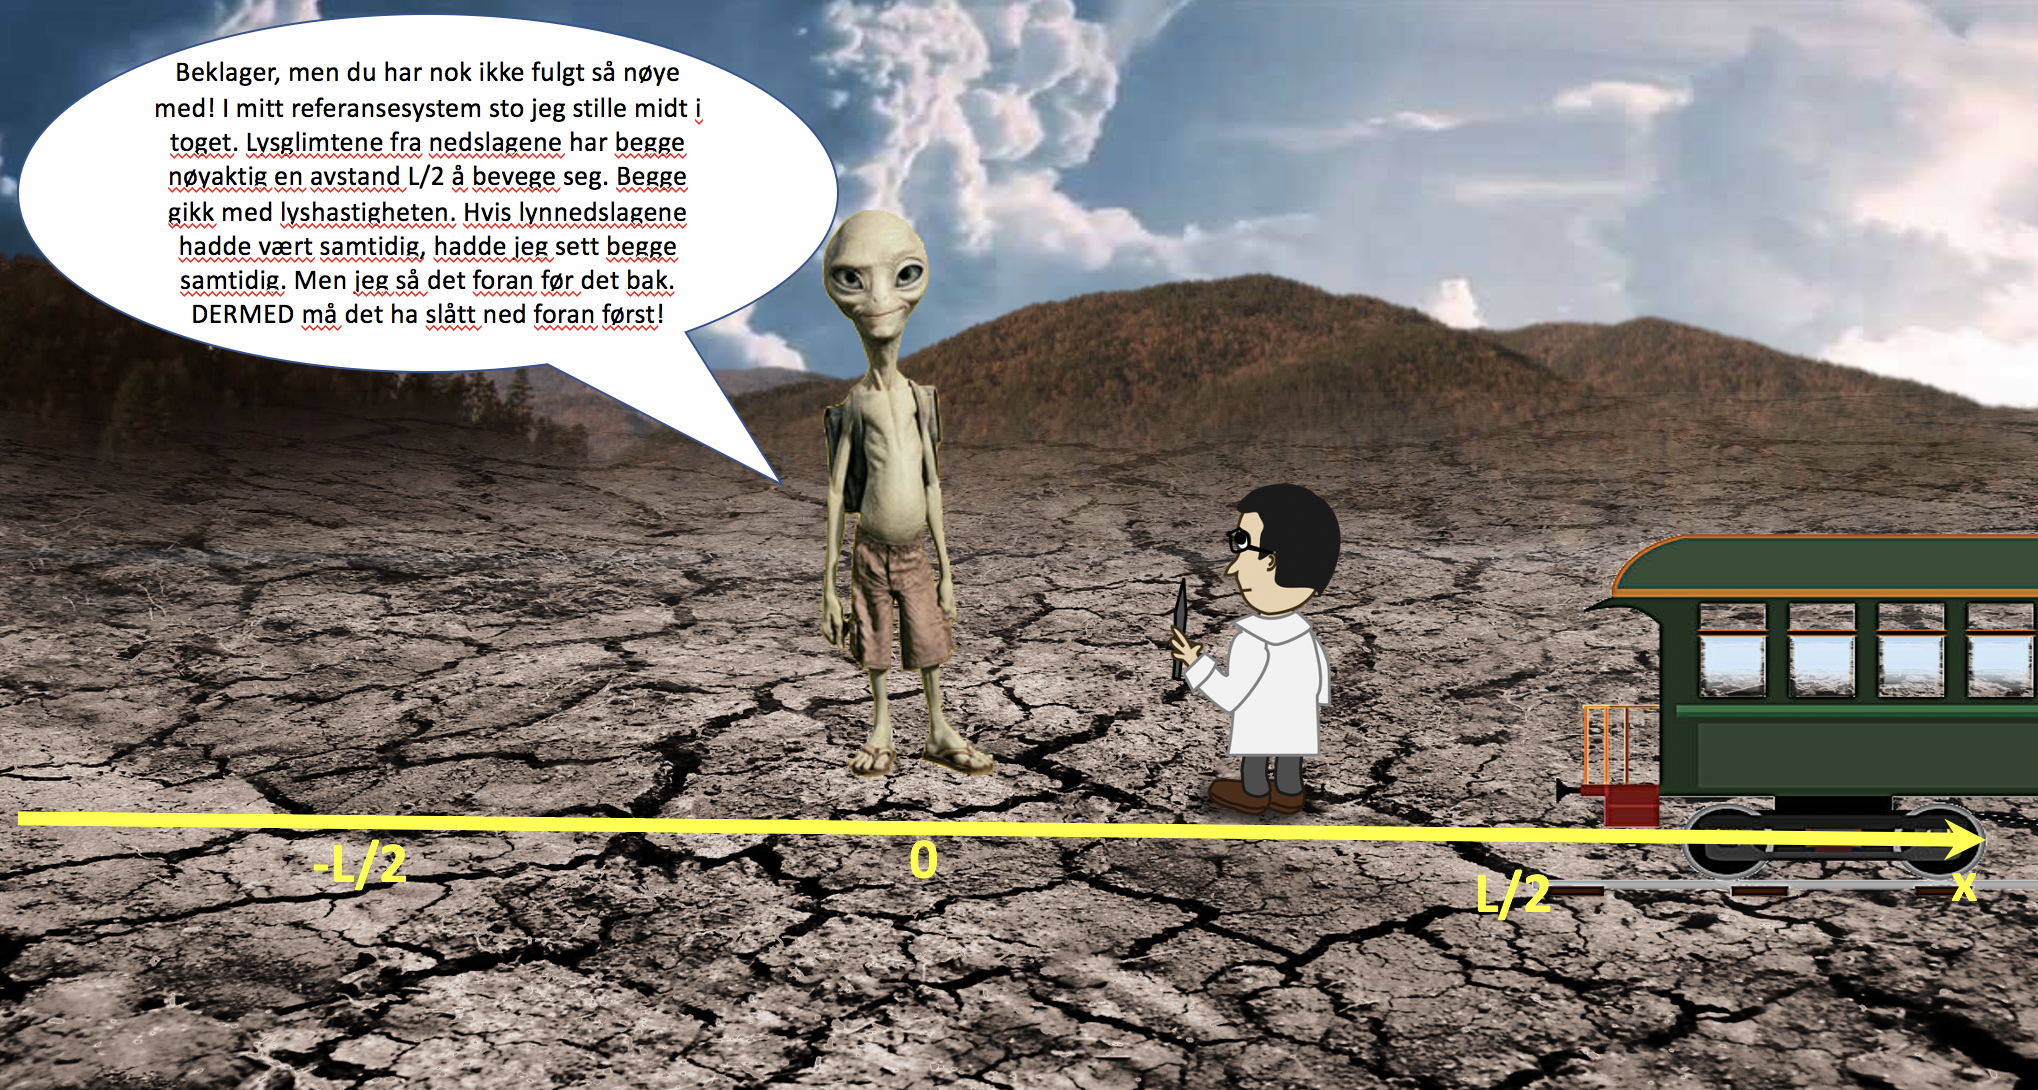
\includegraphics[scale=0.4]{media/samtale4.png}}
}{SIDE 51/61/61}

\fullframe{tog19}{tog18}{tog20}{0}{\Huge
Hvem har rett??? Hva skjedde egentlig??? Diskuter i 5-10 minutter.
}{SIDE 52/61/61}

\fullframe{tog20}{tog19}{tog21}{0}{\Huge
Einstein så kun to mulige løsninger på dilemmaet. Gjør du?
}{SIDE 53/61/61}

\fullframe{tog21}{tog20}{tog22}{0}{\huge
{\bf 1)} De fysiske lovene er forskjellige i de forskjellige referansesystemene. Vi får feil svar, fordi vi har brukt de samme fysiske lovene i begge referansesystem når vi har regnet. Men hvordan skal vi vite hvilke fysiske lover gjelder i hvilket referansesystem? Hvis det ikke finnes et absolutt referansesystem som vi kan definere alle andre fra, da er dette en umulig løsning.
}{SIDE 54/61/61}

\fullframe{tog22}{tog21}{tog23}{0}{\large
Einstein gjorde det helt klart at dette ikke var en løsning gjennom å postulere
\begin{block}{Relativitetsprinsippet}
De fysiske lovene er de samme i alle referansesystemer i {\bf fri flyt.} Vi skal senere komme mer nøyaktig tilbake til hva fri flyt betyr. For nå så betyr det alle referansesystemer som det ikke virker krefter på og som dermed har konstant hastighet. Det vil si at alle fysiske lover som man finner ved eksperimenter i et referansesystem i fri flyt, vil være like gyldige i ethvert annet referansesystem i fri flyt selv om det ikke har samme hastighet som referansesystemet der. Alle referansesystemer i fri flyt er ekvivalente.
\end{block}
Vi kjenner allerede til at de fysiske lovene {\bf ikke} er like for referansesystemer som er akselererte: da får du plutselig fiktive krefter.
}{SIDE 55/61/61}

\fullframe{tog23}{tog22}{tog24}{0}{\large
Med bakgrunn i relativitetsprinsippet, sto Einstein igjen med kun en tenklig løsning på dilemmaet:
\begin{block}{2: Samtidighet er et relativt begrep}
Noe som er samtidig i et referansesystem er ikke samtidig i et annet. Dermed kunne begge observatørene ha rett: lynnedslagene var samtidig for referansesystemet til professor O. Men i passasjer P sitt referansesystem, skjedde lynnedslaget foran først! \textcolor{white}{Og vi snakker ikke om en tilsynelatende effekt: I togsystemet så {\bf slo lynet ned foran først}, punktum! Det ene er ikke riktigere enn det andre, {\bf samtidighet er relativt.}} Samtidighet er dermed like relativt som hastighet: Akkurat på samme måte som den observerte hastigheten til et objekt avhenger av hvilket referansesystem den måles fra, så er samtidighet også noe som avhenger av referansesystmet.
\end{block}
}{SIDE 56/61/61}


\fullframe{tog24}{tog23}{tog25}{0}{\large
Einsteins to postulater her, relativitetsprinsippet og det at samtidighet er relativt var på den tiden kun {\bf postulater}. Det Einstein gjorde var å utrede konsekvensene av disse postulatene. Dette ga oss relativitetstteorien. {\bf Kun gjennom verifikasjon i eksperimenter kan vi vite om disse postulatene er riktige.} I dag, over 100 år og utallige eksperimenter senere {\bf har Einsteins relativitetsteori fått kraftig støtte} i empiriske data fra eksperimenter. \textcolor{red}{\bf Husk at en vitenskaplig teori aldri kan bevises, den kan kun motbevises (falsifiseres).} Men en teori slik som relativitetsteorien som har blitt bekreftet gang på gang og aldri blitt falsifisert blir etterhvert en etablert teori selv om vi aldri kan vite 100\% sikkert om den er helt gyldig. Vi vet idag at Newtons tyngdelov kun er en enormt god tilnærmelse i svake tyngdefelt, men Einsteins generelle relativitetsteori er en tyngdelov som passer bedre med eksperimenter. Det betyr ikke at vi betrakter Newtons lover som gale, kun at de er gyldig bare for svake gravitasjonsfelt.
}{SIDE 57/61/61}


\fullframe{tog25}{tog24}{tog25b}{0}{\huge
Merk videre at postulatet om at samtidighet er relativt kun er en følge av postulatet (med sterk empirisk støtte) om at lyshastigheten er den samme for alle observatører kombinert med relativitetsprinsippet: Hvis disse to samtidig skal være oppfylt, så må samtidighet være relativt for å unngå selvmotsigelser slik som det med lynnedslagene i toget.
}{SIDE 58/61/61}

\fullframe{tog25b}{tog25}{tog26}{0}{\large
I eksemplet vårt med toget så oppsto dilemmaet fordi vi ikke spesifiserte {\bf for hvilken observatør de to lynnedslagene var samtidige}. \textcolor{red}{Konsekvensen av at samtidighet er relativt er at du {\bf alltid} når du bruker ordet ``samtidighet'' samtidig {\bf må si i hvilket referansesystem noe er samtidig!}}. Vi får vite at passasjer P ser først det ene lynnedslaget og dermed det andre. Da må det betyr at lynnedslagene var samtidig i labsystemet og dermed ikke i togsystemet. De regningene vi gjorde i labsystemet var dermed riktige siden lynnedlagene der faktisk var samtidige. I togsystemet var de ikke det, og regningene og resultatene vi fant der var dermed gale.
}{SIDE 59/61/61}


\fullframe{tog26}{tog25b}{tog27}{0}{\Large
Det at samtidighet er relativt her en rekke dyptgripende konsekvenser. Du kan nå velge, avhengig av preferanse om du vil ENTEN (1) lese om dette i \href{https://www.uio.no/studier/emner/matnat/astro/AST2000/h20/undervisningsmateriell/lecture_notes/part2a.pdf}{de vanlige forelesningsnotatene for del 2A}, det er avsnitt 2 ``Invariance of the spacetime interval`` som er aktuelt 

ELLER (2) se \href{https://www.uio.no/studier/emner/matnat/astro/AST2000/h20/undervisningsmateriell/interaktive-forelesningsnotater/2a/videoer/video2a_3.mp4}{denne videoen} som presenterer det samme stoffet. {\bf Merk at videoen tar en halvtime, sett deg godt til rette i godstolen, forbered en kopp te og gjør deg klar for hårreisende stoff...livet ditt blir ikke det samme etter dette!}
}{SIDE 60/61/61}

\fullframe{tog27}{tog26}{oppsummering}{0}{\large
Du skulle nå ha lært at:
\begin{itemize}
\item et event som skjer i posisjon og tid (x,t) i et referansesystem vil skje på en annen posisjon og et annet tidspunkt (x',t') i det andre referansesystemet.
\item den romlige avstanden $\Delta x$ og tidsintervallet $\Delta t$ mellom de to samme eventene er forskjellige i forskjellige referansesystemer, MEN tidromsintervallet $\Delta s=\sqrt{\Delta x^2-\Delta t^2}$ er den samme.
\item for å kunne regne med tidromsintervall så må avstander i både rom og tid måles i samme enheter, enten meter for begge eller sekunder for begge. Omregningsfaktoren er lyshastigheten $c$.
\end{itemize}
}{SIDE 61/61/61}

\begin{frame}
\label{oppsummering}
\hyperlink{tog27}{\pagebutton{\small Forrige side}}\href{https://nettskjema.no/a/170171}{\Changey[1][yellow]{2} \Changey[1][yellow]{-2}}
{\bf Du er ferdig med forelesning 1 av 2 i del 2A.}. Du bør nå:
\begin{itemize}
\item kunne transformere hastigheter mellom referansesystemer i den klassiske relativitetsteorien
\item kjenne til Michelson-Morley-eksperimentet
\item kjenne til relativitetsprinsippet
\item kunne forklare at lyshastighetens invarians kombinert med relativitetsprinsippet gir oss at samtidighet er relativt
\item kunne forklare at det at samtidighet er relativt gjør at både rom og tidkoordinater til eventer avhenger av referansesystemet
\item kunne forklare hva det betyr at tidromsintervallet er invariant
\item kunne regne om romlige avstander til sekunder eller tidsintervaller til meter
\end{itemize}
\textcolor{red}{Flott hvis du nå kan klikke på smilefjesene over og fortelle hva du synes om dette interaktive forelesningsnotatet. Hva var bra og nøyaktig hva kan forbedres? All ris og ros mottaes med takk!}
\end{frame}



\end{document}
